% set document class as 'report'
% set default font size as '12pt'
\documentclass[12pt]{report}

\usepackage[utf8]{inputenc}

% ====== for reference clickable ======
\usepackage{hyperref}
% ====== for graphics ======
\usepackage{graphicx} % includegraphic 
\usepackage{placeins} % FloatBarrier 
% ====== set Font Family ======
\usepackage{mathptmx} % Font: Times
% ====== set margin here ======
\usepackage{geometry}
\geometry{
 a4paper, % set A4 paper
 right=1in, % set margin 1 inch
 bottom=1in, % set margin 1 inch
 top=1in, % set margin 1 inch
 left=3cm % set margin 1.5 inch
 }
% ====== for styling Table of Content =====
\usepackage{tocloft}
% ====== for styling 'chapter' and 'section' ...
\usepackage{titlesec}

\usepackage{gensymb}
\usepackage{subfig}
\usepackage{amssymb,amsthm,amsmath}
\usepackage{algorithm}
\usepackage{algcompatible}
% Chapter
\titleformat
{\chapter} % command
[display] % shape
{\bfseries\large\center} % format
{CHAPTER \thechapter} % label
{0.6em} % sep
{} % before-code
[] % after-code
% remove space above and set below 28pt space chapter
\titlespacing*{\chapter}{0pt}{-35pt}{28pt}

% Section (Heading, Level 2)
\titleformat
{\section} % command
[hang] % shape
{\bfseries} % format
{\thesection} % label
{0em} % sep
{ } % before-code
[] % after-code
% add 1.5 line space above section and remove line space after it
\titlespacing*{\section}{0pt}{1.6em}{0pt}

% subSection (Heading, Level 3)
\titleformat
{\subsection} % command
[hang] % shape
{\bfseries \itshape} % format
{\thesubsection} % label
{0em} % sep
{ } % before-code
[] % after-code
% add 0 line space above section and remove line space after it
\titlespacing*{\subsection}{0pt}{0em}{0pt}

% subsubSection (Heading, Level 4)
\titleformat
{\subsubsection} % command
[runin] % shape
{\bfseries} % format
{\thesubsubsection} % label
{0em} % sep
{ } % before-code
[] % after-code
% 0.5inch indent, 0 line space above, 1 space after header
\titlespacing*{\subsubsection}{0.5in}{0em}{1ex}

% ====== Indent ======
% By default, the first paragraph is not indent - we need this package for indentation
\usepackage{indentfirst}
% ====== list + enum ======
\usepackage{enumitem}
% Set indent lenght for itemize and enumerate
\setlist[itemize]{left=0.5in}
\setlist[enumerate]{left=0.5in}
% Remove separation between item
\setlist{nosep}
% ====== caption styling ======
\usepackage{caption}
\DeclareCaptionFormat{aitformat}{\textbf{#1} #2 \textit{#3}}
% justification = RaggedRight : Caption start on the left
% singlelinecheck = false     : Force caption to start on the left
% labelsep = newline          : separate Table 1.1 and label
\captionsetup{format = aitformat,
              justification = RaggedRight,
              singlelinecheck = false,
              labelsep = newline}
              
% ====== References ======
\usepackage[notocbib]{apacite}

% ====== Document begins here ======
\begin{document}
    % Set counter depth up to subsubsection (heading, level 4)
    \setcounter{secnumdepth}{3}
    
    % ====== include other section ======
    \begin{titlepage}
%   everything on center
  \begin{center}
   
  \textbf{\large{
  AUTONOMOUS MULTI-AGENT AERIAL MAPPING USING STRUCTURE FROM MOTION AND WIRELESS MESH NETWORKS
  }}

  \vspace{3em} % (3 blank lines)
  
  by
  
  \vspace{3em} % (3 blank lines)
  
  Raunak Mukhia
  
  \vspace{4em} % (4 blank lines)

  A Thesis Submitted in Partial Fulfillment of the Requirements for the Degree of Master in Engineering in Computer Science

  \vspace{4em} % (4 blank lines)

\begin{center}
  \begin{tabular}{ rl }
Examination Committee: & Prof.\ Matthew N. Dailey (Chairperson) \\
                       & Dr.\ Adisorn Lertsinsrubtavee \\ 
                       & Dr.\ Mongkol Ekpanyapong \\\\
                       
% UNCOMMENT THE LINES BELOW IF YOU HAVE THE EXTERNAL EXAMINER.
% External Examiner: & Prof. YOUR EXTERNAL EXAMINER  \\
%                   & Dept. of Electrical and Computer Engineering \\ 
%                   & McGill University, Canada \\ \\
\\ \\ \\
Nationality:     & Indian \\
Previous Degree: & Bachelor of Technology in Computer Science and Engineering \\
                 & Sikkim Manipal Institute of Technology \\
                 & India \\
\\
% *  For Self-Support – delete the line Scholarship Donor
Scholarship Donor: & AIT Fellowship
  \end{tabular}
\end{center}

\vspace{4em}

Asian Institute of Technology \\
School of Engineering and Technology \\
Thailand \\ 
% (month and year of graduation)          
May 2021


  \end{center}
\end{titlepage}

    
    % Show page numbering as 'roman'
    \pagenumbering{roman}
    % Start page counter as 2
    \setcounter{page}{2}
    
    % add to Table of content
\addcontentsline{toc}{part}{ACKNOWLEDGMENTS}

% set 0 indentation
\setlength{\parindent}{0pt}
% set paragraph space = 1 space
\setlength{\parskip}{1em}
% set line space = 1
\setlength{\baselineskip}{1.2em} % this is the default value for line space = 1

\begin{center}
  \fontsize{14}{17}\selectfont{\textbf{
    ACKNOWLEDGMENTS
  }} \\
\end{center}
\vspace{36pt} 

I hold sincere gratitude towards my faculty advisor, Dr. Matthew N. Daily for his guidance, encouragement, and direction. I am extremely grateful to him for supporting my study, taking the time to review and correct my report, and for providing me with equipment even outside working hours. I would also like to extend my deepest gratitude to my examination committee members, Dr. Adisorn Lertsinsrubtavee and Dr.  Mongkol Ekpanyapong for their suggestions and time throughout the study. I would also like to express my deepest appreciation to Dr. Lertsinsrubtavee for his constant support and guidance. My thesis would not have been possible without Dr. Daily and Dr. Lertsinsrubtavee. 

I am deeply indebted to IntERLab for providing me with the infrastructure and networking equipment to complete my study.  I would like to express my heartfelt appreciation to Nunthaphat Weshsuwannarugs, Kalana Jayaratne, and Nisarat Tansakul for their help towards making the study realize into a real drone with a mesh network towards the end of my study. 

I would like to thank our CSIM secretary, Sireekant Thanwongpan, for scheduling and arranging presentation dates with my examination committee.

I also thank my parents, family, and friends who encouraged and supported me throughout the time of my study. I and extremely grateful to my mother for her continuous support and motivation to complete my study.
    % add to Table of content
\addcontentsline{toc}{part}{ABSTRACT}

% set 0 indentation
\setlength{\parindent}{0pt}
% set paragraph space = 1 space
\setlength{\parskip}{1em}
% set line space = 1.5
\setlength{\baselineskip}{1.5em}

\begin{center}
  \fontsize{14}{17}\selectfont{\textbf{
    ABSTRACT
  }}
\end{center}
\vspace{2em}

Drones have become inexpensive and can be used to survey an area of interest and send real time data to the ground control station. However, low-cost drones suffer from the constraints of limited flight time due to battery limitations. If the region is denied of network infrastructure (cellular network) such as in remote areas or disaster then the range of the drone is limited to the wifi network range. A system that uses multiple drones can be used to survey and acquire real-time data as it reduces the amount of flight time for each drone. The range of the drones can be extended using a wireless mesh network with each drone working as a node of the mesh. 

For such systems, the operator can either set the flight path for each drone before the mission or many operators can fly the drones individually.  However, it becomes the responsibility of the operators that the drones do not collide with each other, and they do not fly beyond the range of the mesh network. The mesh nodes are mobile, therefore the area of coverage of the network is dynamic throughout the mission.

In this study, I propose a centralized system called Pegasus for autonomous exploration and aerial map building with multiple drones using a wireless mesh network. The different phases in the pipeline used in this system to achieve autonomous flight and map building are described.  The pipeline consists of the presentation layer, multi-agent coverage path planning layer, motion control layer, real time image acquisition layer, and map generation layer using structure from motion. To evaluate the system, a simulation framework is presented in this study. Finally, the system is evaluated in the real world with a single drone. 


\textbf{Keywords:} Multi-agent CPP, Wireless mesh network, SfM, Autonomous UAV
    % Rename table of content to CONTENTS
\renewcommand\contentsname{\begin{center}
  \fontsize{14}{17}\selectfont{\bf{CONTENTS}}
\end{center}}
% set space above title
\renewcommand{\cftbeforetoctitleskip}{-35pt}
% set space below title
\renewcommand{\cftaftertoctitleskip}{0em}
% after title, skip 3 spaces and write 'page' on the right
\renewcommand{\cftaftertoctitle}{%
  \vspace{3em}
  \hfill{\textbf{Page}}
}
% Remove . from table of content
\renewcommand{\cftdot}{}

% styling part:
\renewcommand{\cftpartfont}{\fontsize{12}{14}\selectfont\bf} % set font bold for page name
\renewcommand{\cftpartpagefont}{\fontsize{12}{14}\selectfont\bf} % set font size and bold for page number
\setlength{\cftbeforepartskip}{0pt} % set line space

% styling chapter:
\renewcommand{\cftchapfont}{\bf{CHAPTER} \fontsize{12}{14}\selectfont\bf} % set font size bold, leading with 'CHAPTER'
\renewcommand{\cftchappagefont}{\fontsize{12}{14}\selectfont\bf} % set font size and bold for page number
\setlength{\cftbeforechapskip}{0pt} % set line space
\setlength{\cftsecindent}{4.5em}
\setlength{\cftsubsecindent}{7em}

% set dept of contents
\setcounter{tocdepth}{2}

% Print content
\tableofcontents
    \addcontentsline{toc}{part}{LIST OF TABLES}

% Rename List of Tables to CONTENTS
\renewcommand\listtablename{\begin{center}
  \fontsize{14}{17}\selectfont{LIST OF TABLES}
\end{center}}
% set space above title
\renewcommand{\cftbeforelottitleskip}{-25pt}
% set space below title
\renewcommand{\cftafterlottitleskip}{0em}
% after title, skip 3 spaces and write 'page' on the right
\renewcommand{\cftafterlottitle}{%
  \vspace{3em}
  \textbf{Tables}\hfill{\textbf{Page}}
}

% remove indent
\renewcommand{\cfttabindent}{0pt}
% add 'Table' before numbering
\renewcommand{\cfttabpresnum}{Table~}
% indent the table caption
\renewcommand{\cfttabnumwidth}{4.5em}

\begingroup
    \renewcommand*{\addvspace}[1]{}
    \listoftables
\endgroup
    \addcontentsline{toc}{part}{LIST OF FIGURES}

% Rename List of Tables to CONTENTS
\renewcommand\listfigurename{\begin{center}
  \fontsize{14}{17}\selectfont{LIST OF FIGURES}
\end{center}}
% set space above title
\renewcommand{\cftbeforeloftitleskip}{-25pt}
% set space below title
\renewcommand{\cftafterloftitleskip}{0em}
% after title, skip 3 spaces and write 'page' on the right
\renewcommand{\cftafterloftitle}{%
  \vspace{3em}
  \textbf{Figures}\hfill{\textbf{Page}}
}

% remove indent
\renewcommand{\cftfigindent}{0pt}
% add 'Table' before numbering
\renewcommand{\cftfigpresnum}{Figure~}
% indent the table caption
\renewcommand{\cftfignumwidth}{4.5em}

\begingroup
    \renewcommand*{\addvspace}[1]{}
    \listoffigures
\endgroup
    
    % Start page counter as 1
    \setcounter{page}{1}
    % Show page numbering as 'arabic'
    \pagenumbering{arabic}
    % set 0.5 inch indentation
\setlength{\parindent}{0pt} 
% set paragraph space = 0 space
\setlength{\parskip}{0mm}
% set line space 1.5
\setlength{\baselineskip}{1.6em}

\chapter{INTRODUCTION} 

\section{Background of the Study}

The availability and financial accessibility of unmanned aerial vehicles (UAVs) have made them more widespread, with applications ranging over a wide range of civilian activities. Multi-rotors are used for recreational flying, research, cinematography, disaster observation, logistics, agriculture,  public safety, construction, surveillance, and environmental protection, amongst other purposes. 

A cluster of inexpensive autonomous multi-rotors connected through a wireless mesh network that can be deployed in a post-disaster situation could help avoid dangerous situations faced by ground-based human observers in such scenarios. The drones should be able to perform aerial mapping quickly, as they can coordinate so that one drone does not need to visit locations already visited by other drones in the cluster. The range of the cluster can also be large, since each drone would act as a wireless mesh access point. At the same time, each drone could act as an access point to provide connectivity in the disaster-stricken area.  

Aerial mapping drones can be outfitted with an array of sensors such as ultrasonic sensors, infrared sensors, multi-array laser sensors, and RGB-D cameras. However, systems with many sensors will suffer from integration complexity, weight constraints, reduced battery lifetime, and high cost. Structure from motion (SfM) using monocular cameras attached to each drone provides a low cost, lightweight, simple alternative to sensor-intensive approaches. 

This study proposes a system for command and control of a cluster of autonomous drones, each being a node in a wireless mesh network, controlled from a centralized control station that oversees coordinated exploratory path planning and aerial mapping using SfM.

\section{Statement of the Problem}

An inexpensive cluster of UAVs providing autonomous coordinated aerial mapping after a disaster can be a valuable asset for disaster observation and public safety that does not pose any risks for ground-based surveillance personnel. Multiple drones will reduce flight time and increase the spatial extent of the SfM result. A wireless mesh network can also be an inexpensive solution when communication infrastructure such as cellular data services are dysfunctional. Increasing the number of drones in the system can enable increased range of the mesh network, because each drone acts as a mesh node. Providing emergency network services using UAVs and mesh networks in disaster-stricken areas is an active research area, as discussed by \shortciteA{Chand2018}, but the best method to combine coverage for mapping while maintaining mesh connectivity is an open problem. \shortciteA{Sabino2018} discuss optimal placement of UAVs in a mesh network, and separately, a survey of the multi-agent coverage path planning problem (CPP) by \shortciteA{Almadhoun2019} reviews many CPP methods proposed in the literature. However, the requirement for mesh network connectivity imposes severe constraint on the movement of agents, making the resulting "constrained CPP" an open research area.

Simulation environments exist that can be used for multi-drone planning and wireless mesh networks. Pixhawk PX4's software in the loop (SITL) along with Gazebo can simulate a physical fleet of UAVs with cameras. Wireless mesh networks can be simulated by Network Simulator 3 (NS3). The Robot Operating System (ROS), with its range of tools and available packages, provides a strong platform to develop this system. FlySimNet by \shortciteA{Baidya2018} is a UAV network simulator created by combining NS3 and Ardupilot's UAV SITL simulator with lightweight publish/subscribe (ZMQ) based middleware. It uses a custom graphical ground control system (GCS) application that communicates via the ZMQ messaging service, which does not support ROS, and cameras are not supported by Ardupilot SITL. The CORNET middleware framework by \shortciteA{AcharyaRBCCPS} combines Gazebo, NS3 and PX4, but it is available only as a published paper and implementation of their method is not quite clear. Neither of these frameworks implement wireless mesh network simulation on NS3. Gazebo, NS3, PX4, and ROS together provide an open source platform, but integration of these tools is required.

This thesis aims to design and implement a multi-agent CPP method that satisfies wireless mesh network constraints, runs multi-agent SfM. It also aims to develop a simulation framework to support the CPP method.

\section{Objectives of the Study}

The main objective of this thesis is to improve on the state of the art in mapping disaster-stricken areas by designing and implementing a method for autonomous control of a multi-agent exploration and coordinated aerial mapping team performing SfM. The focus of this study is to map a disaster-stricken area with the possible damage to communication infrastructure; therefore, the system will use a wireless mesh network for internal communication, with each agent working as a mesh node. The objectives can be decomposed into the following specific tasks:
\begin{itemize}
	\item Design and implement a user-friendly pipeline utilizing the Robot Operating System (ROS) that allows the operator to select an area to survey.
	
	\item Design and implement strategies to find the transformations between the global map and the local map of each drone continuously such that the control station can coordinate the position of each drone with respect to the global map.
	
	\item Design and implement a method for establishing a reliable communication channel between each drone and the control station over the mesh network.
	
	\item Design and implement an autonomous exploration and coordination system for the agents that operates within the restriction of the range of the wireless mesh network. The system should maximize the extent of the mappable area, by planning an appropriate arrangement of agents over time.
	
	\item Implement a multi-agent SfM method capable of generating an aerial map of the area under surveillance.
	
	\item Design and implement a simulation framework for the entire system using PixHawk PX4 as the drone flight controller, Gazebo and Network Simulator 3 as simulation tools, ROS for overall coordination, and useful robotics/vision algorithms.
	
	\item Design and implement a wireless mesh network with each drone as a mesh node. As the drones are fast-moving agents, this will require the study and implementation of solutions to maintain a reliable network with a usable quality of service, despite constant topology changes.
	
	\item Evaluate the system's ability to execute effectively in the real world.
\end{itemize}

\section{Limitations and Scope}

The study will not cover the following.
\begin{itemize}
	\item \textit{Obstacle detection and avoidance}: The control station will generate paths for the drones, such that they will not collide with each other. It is assumed that no unknown obstacle will be present at the drone's operational altitude. It is the operator's responsibility to indicate the minimum altitude during mapping.
	
	\item \textit{Dynamic path reconfiguration}: The control station will generate complete paths for the drones before the start of the mission.
	
	\item \textit{Recovery mechanism}: If communication is lost with any drone, it will return to the home position using the default behavior in PX4. The remaining drones will continue their operation.
	
	\item \textit{Global Positioning System failure}: It is assumed that GPS will be continuously functional.
	
	\item \textit{Number of drones in evaluation}: The simulation environment have been tested with a maximum of three drones, real world validation uses only one drone.
\end{itemize}

\section{Organization of the Thesis}

The thesis is organized as follows:
\begin{itemize}
	\item Chapter \ref{ch:literature-review} provides a literature review related to this study.
	\item Chapter \ref{ch:methodology} proposes the methodology for the system developed in this study.
	\item Chapter \ref{ch:results} presents experimental results using the system developed in this study.
	\item Finally, chapter \ref{ch:conclusion} concludes the thesis and provides recommendation for future work.
\end{itemize}

\FloatBarrier

    % % set 0.5 inch indentation
\setlength{\parindent}{0.5in} 
% set paragraph space = 0 space
\setlength{\parskip}{0mm}
% set line space 1.5
\setlength{\baselineskip}{1.6em}

\chapter{TITLE}
Write your introductory paragraph/s here (except for Chapter 1). Limit this section to two paragraphs. Follow the appropriate structure of writing paragraphs. Paragraphs should have at least four sentences. Paragraphs with more than 6 sentences must be split into two paragraphs.

\section{Heading, Level 2}
Start your paragraph here.
\section{Heading, Level 2}
Start your paragraph here.
\subsection{Heading, Level 3}
Start your paragraph here.
\subsection{Heading, Level 3}
Start your paragraph here.
\section{Heading, Level 2}
Start your paragraph here.
\subsection{Heading, Level 3}
Start your paragraph here.
\subsection{Heading, Level 3}
Start your paragraph here.
\subsubsection{Heading, Level 4}
Start on the same line here and continue as a regular paragraph.
\subsubsection{Heading, Level 4}
Start on the same line here and continue as a regular paragraph.
\section{Heading, Level 2}
Start your paragraph here.
    % set 0.5 inch indentation
\setlength{\parindent}{0.5in} 
% set paragraph space = 0 space
\setlength{\parskip}{0mm}
% set line space 1.5
\setlength{\baselineskip}{1.6em}

\chapter{LITERATURE REVIEW}
\label{ch:literature-review}

\textit{This chapter begins with a review of the functional architecture of autonomous driving systems, coordinate systems, the PixHawk, and ROS coordinate conventions.} 

\section{Software Architecture of Autonomous Driving Vehicles}
\label{section-name-in-literature-review}

\shortciteA{sbehere16t} splits the major components of the motion control part of autonomous driving systems into three main categories as shown in Figure~\ref{fig:fav_automonous}. These categories are:

\begin{itemize}
	\item Perception of the external environment in which the vehicle operates
	\item Decision making and control of vehicle motion with respect to the external environment that is perceived
	\item Vehicle platform manipulation, which deals mostly with sensing, control, and actuation of the vehicle, with the intention of achieving the desired motion.
\end {itemize}

Each category can be further broken down into several components. I describe each component in more details in the following sections.

\subsection{Perception}

Sensing components sense the state of the vehicle and the state of the environment in which the vehicle operates. The sensor fusion component considers multiple sources of information to construct a hypothesis or belief about the state of the environment. The localization component determines the location of the vehicle with respect to a global map. The semantic understanding component processes the sensor input and derives meaningful information from it. The world model component holds the current estimate of the state of the external environment.

\subsection{Decision and Control}
The trajectory generation component repeatedly generates a set of obstacle-free trajectories in the world coordinate system and picks an optimal trajectory from the set. Energy management components deal with energy management of the vehicle. Diagnosis and fault management monitors the state of the overall system and its components. Reactive control components are used for immediate responses to unanticipated stimuli from the environment. The vehicle platform abstraction component refers to a minimal model of the vehicle platform. 

\subsection{Vehicle Platform Manipulation}

The platform stabilization component's task is to keep the vehicle platform in a controllable state during operation. Trajectory execution components are responsible for executing the trajectory generated by the decision and control component. 

\begin{figure}
	\centering
	\caption[FAV of Antonomous Driving System.]{\small 
		Functional architecture of an autonomous driving system. Reprinted from Behere (2016). }
	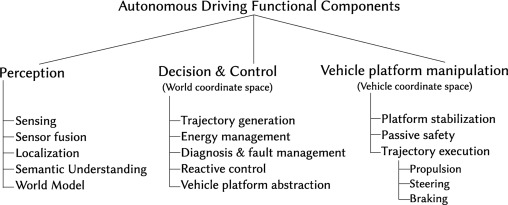
\includegraphics[width=5in]{figures/literature/fav_autonomous_driving}
    \label{fig:fav_automonous}
\end{figure}

\section{Coordinate Systems}

In this section I describe the different coordinate system conventions in use in robotic applications. 
	
\subsection{Earth Centric, Earth Fixed}

The earth-centered earth-fixed (ECEF) coordinate system, rotates with the Earth and has its origin at the center of the Earth. Refer to Figure~\ref{fig:coordinatesystem} (a) for a visualization. ECEF follows the right-handed coordinate system convention. \shortciteA{coordinatesystem} describes ECEF as follows.

\begin{itemize}
	\item The origin is at the center of mass of the Earth, a point close to the Earth's center.
	\item The Z axis is on the line between the magnetic north and south poles, with positive values increasing northward (but not exactly coinciding with the Earth's rotational axis).
	\item The X and Y axes lie in the plane of the equator.
	\item The X axis passes through the point on the equator from 180 degrees longitude (negative) to the prime meridian (0 degrees longitude, positive).
	\item The Y axis passes through the point at 90 degrees west longitude along the equator (negative) to 90 degrees east along the equator (positive).
\end{itemize}

\subsection{World Geodetic System}
The World Geodetic System is a standard system used in GPS, cartography and geodesy. The latest revision is WGS 1984 (WGS 84) that was established and is maintained by the United States National Geospatial-Intelligence Agency. It was last revised in 2004. The World Geodetic System 1984 (WGS 84) is one of the best global geodetic reference system for the Earth available presently. The datum (ellipsoid) defined by WGS 84 is generally used to convert the GPS latitudes and longitude to the UTM coordinate system.

\subsection{Universal Transverse Mercator Geopraphic Coordinate System}
The Universal Transverse Mercator (UTM) is a coordinate system that divided the earth into 60 zones. Each zone is a plane with its own x and y coordinates in meters. It ignores altitude and treats the earth as a perfect ellipsoid. A UTM coordinate has:

\begin{itemize}
        \item A zone number.
        \item A hemisphere (N/S).
        \item An easting (X coordinate).
        \item A northing (Y coordinate)
\end{itemize}

A coordinate 14.08057584 \degree N, 100.61284553 \degree E in latitude and longitude is represented as 47 N 674132 1557234 in UTM.

\subsection{Local tangent plane}

In the local tangent plane coordinate system, a position on the earth is fixed about the origin. There are two conventions as shown in Figure~\ref{fig:coordinatesystem} (b).

\begin{itemize}
	\item X=East, Y=North, Z=Up (ENU).
	\item X=North, Y=East, Z=Down (NED), which is commonly used in aviation, as the objects of interest usually lie before an aircraft (down or positive Z).
\end{itemize}

\begin{figure}%
	\centering
	\caption[ECEF coordinate system]{\small Coordinate systems. (a) Earth centric, earth fixed (ECEF) coordinate system. (b) Local tangent plane coordinate systems. Reprinted from Krishnavedala. 
	}%
	\subfloat []{{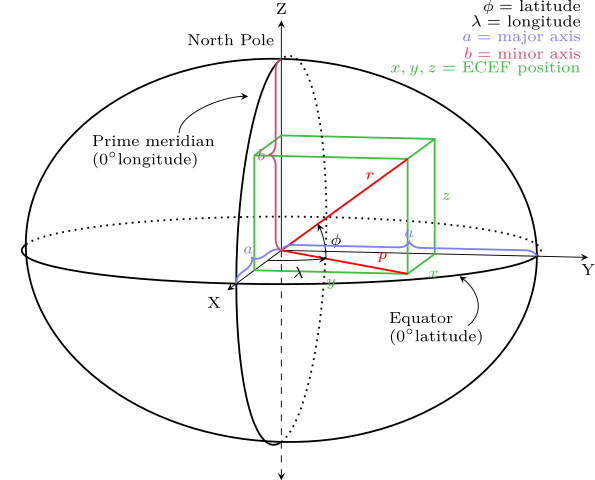
\includegraphics[width=3in]{figures/literature/ECEF}}}%
	\subfloat []{{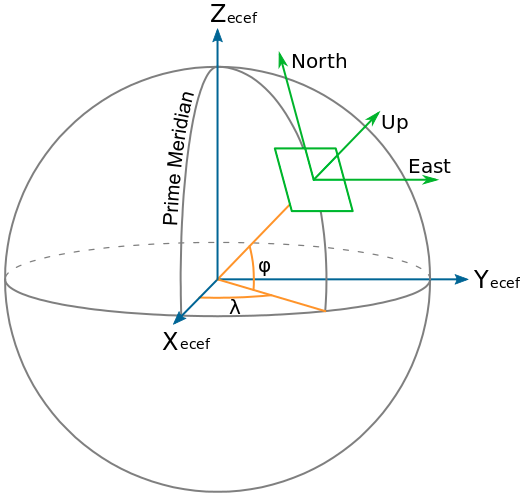
\includegraphics[width=3in]{figures/literature/ENU_NED}}}%
	\label{fig:coordinatesystem}%
\end{figure}

\subsection{PixHawk and ROS coordinate systems}

PixHawk follows the NED convention, whereas ROS follows the ENU convention. The conversion between these different conventions is handled automatically by MAVROS. To translate air-frame related data, a rotation of $180^{\circ}$ degrees is applied about the roll (X) axis. For local data, a $180^{\circ}$ rotation is applied about the roll (X) and $90^{\circ}$ rotation is applied about the yaw (Z) axes.

It is good practice in ROS to set up reference frames as described by \shortciteA{rosrefframes}, shown in Figure~\ref{fig:rosrefframes}.

\begin{itemize}
	\item The coordinate frame called base\_link is rigidly attached to the mobile robot base. It can be attached in any arbitrary position or orientation.
	\item The coordinate frame called odom is a world-fixed frame. The pose of a robot is continuous in this frame, but it can drift over time.
	\item The coordinate frame called map is a world fixed frame, with Z-axis pointing upwards. 
	\item The coordinate frame called earth is the origin of the ECEF frame.
\end{itemize}

\begin{figure}
	\centering
	\caption[Relation between ROS frames]{\small 
		Relationship between ROS frames. Reprinted from \shortciteA{rosrefframes}. }
	
\includegraphics[width=5in]{figures/literature/ros_rel_frames}
	\label{fig:rosrefframes}
\end{figure}

\section{Wireless Mesh Network}

A wireless mesh network's (WMN) consists of two types of nodes, mesh routers and mesh clients. Mesh routers form the mesh backbone for mesh clients. Every node in the mesh has the capability to route packets forward for other nodes if the packet destination is not in direct wireless transmission range. Mesh routers provide functionality as bridge/gateway that enables the WMN to integrate with other networks such as cellular, ad-hoc and ethernet. In a wireless mesh network, all the participating nodes automatically establish and maintain mesh connectivity and are in effect dynamically self-organized and self-configured. WMN can be rapidly deployed where there is no network coverage and has the potential for application in disaster management.

\subsection{WMN Network Architecture}

A wireless mesh network has two types of nodes, mesh routers and mesh clients. Mesh routers can have multiple networking interfaces to provide bridge/gateway functionality to the mesh network and have additional routing functions to support mesh networking. Mesh routers can be built on similar hardware platform as a conventional wireless router. Mesh routers can be build based upon embedded systems and general-purpose computer systems. Mesh clients have capability for mesh networking and can also work as a mesh router, nevertheless they lack bridge/gateway function and usually have only one wireless interface.


The architecture of WMNs can be classified into three types based upon the composition of mesh routers and clients.

\begin{itemize}
	\item \textit{Infrastructure/Backbone WMNs.}
	In this architecture mesh routers form an infrastructure for clients that connect to them. The mesh routers automatically establish and maintain links between themselves and provide gateway functionality to connect the mesh network to other networks and the internet. 
	
	\item \textit{Client WMNs.} In this architecture, mesh routers are not required for maintaining a mesh network. Mesh clients provide peer-to-peer networking, performing routing and configuration management. A packet may reach the destination node through multiples hops through client nodes.
	  
	\item \textit{Hybrid WMNs.} In this architecture, mesh routers provide infrastructure backbone with access to other networks. Client nodes can connect to the mesh network through meshing with other clients, as well as through mesh routers. This in effect, is a combination of infrastructure and client WMNs, and provides increased connectivity and coverage.
\end{itemize}

\subsection{Features of WMNs}

WMNs have redundant nodes and can provide high level of fault tolerance and robustness. If the case of link failure, the mesh network can adapt and reroute the data. Using multi-hop strategies, the coverage range can be increased, as intermediate router and clients can relay packets between hosts which do not have a direct line of sight. WMNs can be rapidly deployed with less maintenance because of self-forming, self-healing and self-organization capability. They are compatible with ad-hoc wireless clients.


\subsection{Routing Protocols for WMNs}

WMNs has redundant and mobile clients, hence, the routing protocols should find and maintain routes between the source and destination nodes by detecting and responding to changes in network topology. Ideally routing protocols should maximize the capacity of the network and minimize the packet delivery delays by creating and selecting efficient routes between nodes.

Wireless mesh routing protocols can be classified into three categories:

\begin{itemize}
	\item \textit{Proactive Routing Protocol.} Proactive routing protocols build and maintain the routing table by sharing routing data among nodes at periodic intervals. It selects the route from the routing table while forwarding packets from one node to the other. Optimized Link State Routing Protocol (OLSR) and Better Approach to Mobile Ad-hoc Networks (BATMAN) falls under this category.
	\item \textit{Reactive Routing Protocol.}  Reactive routing protocols searches the route from source to destination node on demand as it is required. Examples of this category are Ad Hoc On-Demand Distance Vector Protocol (AODV) and Dynamic Source Routing Protocol (DSR).
	\item \textit{Hybrid Routing Protocol.} Hybrid Routing Protocol uses both reactive and proactive routing strategies depending upon the environment. As a reactive routing protocol, it will provide the path on demand, based on up-to-date information. Examples of hybrid routing protocols are ZRP (zone routing protocol), HSLS (hazy sighted link state routing protocol).
\end{itemize}

\subsubsection{Comparision of Routing Protocols}

\shortciteA{Mbarushimana2007} does a comparative study between the performance of reactive (AODV and DSR) and proactive (OSLR) protocols. They run simulations for 1000 seconds, considering four different scenerios, namely, workload, number of flows, number of nodes in the network, and node movement speed. The performance of the three routing protocols is measured based on throughput, good-put, routing load and end-to-end delay. They come to the conclusion that OSLR shows the best performance in terms of data delivery ratio and end-to-end delay, and provide insight that network layer tends to drop more packets while reactive protocol is computing the route to the destination. In their study OSLR still outperforms the reactive routing protocols at higher speeds even though it has the highest routing overhead due to its exchange of periodic routing updates.

\shortciteA{Kulla2012} does a performance comparison of OSLR and BATMAN routing protocols in an indoor stairs environment of 5 floor building. They come to the conclusion that both the protocols perform well for one-hop and two-hop communication. The delay and packet loss increased after three hops for static node scenario and after two hops for moving node scenario. BATMAN performs better than OSLR for packet loss metrics because BATMAN buffers packets when routes are unstable. In general, OSLR protocol showed better performance than BATMAN protocol. OSLR shows better performance than BATMAN regarding the delay metrics, which is critical for real-time communication between a cluster of drones.

From these studies of performance comparisons OSLR seems to be the most suited to my use case, as:
\begin{itemize}
	\item Proactive protocols (OSLR) performs better than reactive protocols in terms of data delivery ratio and end-to-end delay.
	\item Reactive protocols tends to drop packets while they are computing the route.
	\item OSLR shows better performance than BATMAN for delay metrics.
	\item Latest information about the drones in the mesh network is more critical than stale information, which means OSLR with less delay is more suited to the use case of my study.
\end{itemize}

\subsection{Optimized Link State Routing Protocol}

Optimized Link State Routing Protocol (OSLR) belongs to the class of link state routing protocol, with optimization for mobile ad hoc networks.  It is a distributed protocol with no central agency that exchanges topology information with other node of the network periodically. Each node maintains a routing table, and is a proactive protocol. When data is to be sent, it refers to the routing table. The route to other nodes are maintained by each node proactively. 

HELLO message is used for link sensing, neighbor detection, and multipoint relay (MPR) selection. HELLO messages are not forwarded by the nodes. The nodes in OSLR use only selected nodes called multipoint relay (MPR) to re-transmit control messages, reducing overhead from control messages flooding the network. Each node in the network selects a set of nodes in its symmetric 1-hop neighborhood called MPR set of that node. Neighbors which do not belong to MPR set of the node receive and process broadcast messages but do not re-transmit it. If an interface of a node has at least one verified bi-directional link with an interface of another node, it is considered as its symmetric 1-hop neighbor. 

Topology Control (TC) message is used to disseminated topology information through the network, using optimized flooding through MPR mechanism. The TC messages distributed to each node is used to calculate routing table in each node.

If a node has multiple interfaces, it must announce, periodically, information describing its interface configuration to other nodes in the network. Multiple Interface Declaration (MID) message is flooded by such nodes using MPR mechanism in the network, and is used for routing table calculations.

Gateway/bridge nodes have non OSLR interfaces connected to external network such as the ethernet. Host and Network Association (HNA) message are periodically broadcasted by such nodes to register such routing information in the routing table.


The role of OSLR is not to forward data packets. It maintains the routing table in each node which is used by the system to perform network layer forwarding function.

\subsection{FANET}

Flying ad hoc network (FANET) is a specialized subset of mobile ad hoc network(MANET). FANET takes into consideration the challenges faced by MANET with flying UAVs as the mesh nodes. FANET can also be classified as a subset of Vehicular ad hoc network (VANET), where the mesh nodes are vehicles on the ground. The relation between MANET, VANET and FANET is given in Figure~\ref{fig:manet-vanet-and-fanet}.

\begin{figure}
	\centering
	\caption[MANET, VANET and FANET]{\small 
		MANET, VANET,and FANET Reprinted from \shortciteA{Tareque2015}. }
	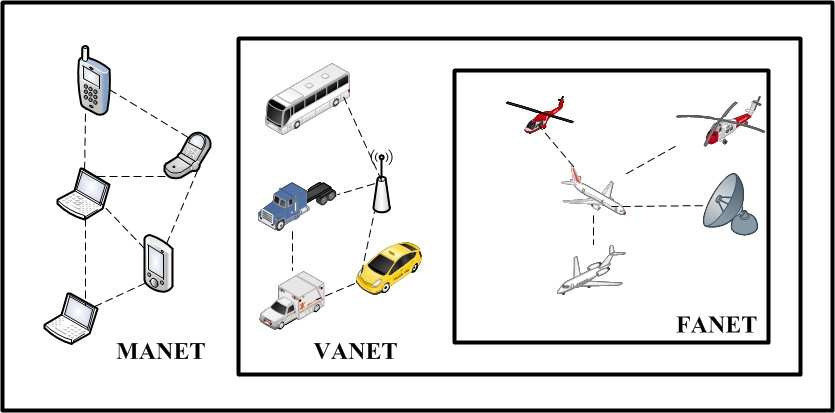
\includegraphics[width=5in]{figures/literature/MANET-VANET-and-FANET}
	\label{fig:manet-vanet-and-fanet}
\end{figure}

Surveys of FANET has been carried out by \shortciteA{Chriki2019} and \shortciteA{Tareque2015}. The challenges of FANET described can be summarized as follows:

\begin{itemize}
	\item \textit{Network topology change.} In FANET, rapidly moving UAVs changes the network topology more frequently.
	\item \textit{Node mobility.} UAVs have a higher degree of mobility than vehicles or people on ground. Node mobility issues can be considered as the most significant difference between FANET and other ad hoc networks.
	\item \textit{Node density.} Node density in FANET is lower than other MANETs. FANET nodes are spread across the sky. There are less number of average nodes in a unit area in FANET. 
	\item \textit{Radio propagation model.} MANET and VANET nodes are close to the ground and because of the environment, they may not have direct line of sight. FANET nodes are in the sky and for most cases have direct line of sight between the nodes.
	\item \textit{Power Consumption.} For large UAVs power consumption is not a significant factor when designing the FANET. However for small UAVs the power consumed by FANET must be taken into consideration.  
	\item \textit{Localization.} UAVs because of its higher mobility degree may have inaccurate GPS position information as compared to other MANETs.	
\end{itemize}

Routing protocols for FANET follows similar classification as WMNs and are as follows:

\begin{itemize} 
	\item \textit{Static protocols.} These protocols have fixed routing tables.
	\item \textit{Proactive protocols.} Updates the routing tables periodically.
	\item \textit{Reactive protocols.} Finds path to the destination node when data needs to be sent.
	\item \textit{Hybrid protocols.}  These use both reactive and proactive strategies when required. 
	\item \textit{Geographic based protocols.} These protocols use position information.
\end{itemize}

There are multiple optimization and extensions for OSLR specifically done to solve challenges for FANET. Some of them are:

\begin{itemize}
	\item \textit{DOLSR.} \shortciteA{Alshabtat2011} proposes Directional Optimized Link State Routing Protocol (DOLSR) which uses directional antenna and heuristic to minimize the number of MPRs. They show reduced end-to-end delay and enhanced overall throughout using DOLSR for FANET.
	\item \textit{P-OSLR.} \shortciteA{Rosati2013} proposes Predictive OSLR (P-OSLR) that uses GPS information to help the routing protocol. It take the relative speed between the nodes in account to calculated expected transmission count (ETX) metric. This metric is used by OSLR for link quality sensing. The show increased multi-hop reliability with minimum outage time as compared to OSLR in FANET environment.
	\item \textit{ML-OSLR.} \shortciteA{Zheng2014} proposes Mobility and Load aware OSLR (ML-OSLR) that introduces mobility and load aware algorithm in the routing protocol. ML-OLSR does not select high speed nodes as the MPR and avoid routing through high load, congested and high speed nodes to increase network stability. They show increased performance in packet delivery ratio and average end-to-end delay compared to OSLR with FANET based simulation.
\end{itemize}

\shortciteA{Singh2015} presents the application of OSLR to FANET under different mobility model of the nodes through simulation. He shows that the increase in speed of nodes decreases throughout, increases end-to-end delay and decreases packet delivery ratio for most mobility model. However, for my study, the speed of the node are relatively low, and nodes spend most of their time waiting for other nodes to arrive to their way-point and take picture, therefore I shall purse the use of generic OSLR for this thesis.


\section{Simulators}

An approximate imitation of a process or system's operation over time is known as simulation. A real-life or hypothetical situation modeled on a computer that captures the behavior of how the system works is a computer simulation. Computer simulation can be a powerful tool to develop, investigate the behavior and save cost, by providing a means to virtually access the system under study.

Some of the classification of simulations are:
\begin{itemize}
	\item \textit{Continuous simulation.} Simulation is based on continuous time and uses numerical integration of differential equations.
	\item \textit{Discrete-event simulation.} Simulation is based on discrete time intervals. The state of the components of the simulation change their value only at discrete time. 
	\item \textit{Stochastic simulation.} Simulation with same input will produce different results within some confidence interval. During simulation some variables or process is subject to random variations.
	\item \textit{Deterministic simulation.} Simulation with same input will always produce the same deterministic results. The variables and process are regulated by deterministic algorithms.
\end{itemize}

\subsection{Computer Network Simulators}

Network simulators are those types of software that are capable of performing predictions on how a computer network will behave. The output of these simulations can be analyzed to derived metrics of the network under consideration. The use of network simulators provide a cost-effective method to validate and optimize the performance of the network before deployment. Network simulators may have the capability for emulation, that is, to pass real packets through the network simulation, and examine the effects of the network on the packets. 

\shortciteA{Siraj2012} has done survey on network simulators (ns-2, ns-3, OPNET, NetSim, OMNet++, REAL, J-Sim and QualNet), their availability, programming languages used and their architecture.  \shortciteA{Toor2017} has done survey on network simulator which can support wireless infrastructure (ns-2, Ns-3, J-Sim, OMNeT++, OPNET, QUALNET and MATLAB) and listed their key features and limitations. \shortciteA{Patel2018} has done survey on network simulator (ns-2, ns-3, OMNeT++, NetSim, REAL, OPNET and QualNet) and listed their features, advantages, disadvantages.

Network Simulator 3 (ns-3) is a discrete-event network simulator, and it's intended uses are for research and education. It is written from scratch using C++ and is not backward compatible with ns-2. NS-3 is a collection of core libraries, modules, and applications which are build using a python based build tool called waf. It can be linked with a user C++ or python application to create a simulation. It is possible to integrate ns-3 with other software through the user application. The architecture of ns-3 is illustrated in Figure~\ref{fig:ns3-architecture}. In this paper I use ns-3 because:
\begin{itemize}
	\item It is intended for scientific research.
	\item It is more flexible than other simulators.
	\item It tries to simulate protocol genuinely.
	\item It is open source and free to use.
	\item It can be integrated with other software.
	\item It is actively developed and maintained. ns-2 development stopped around 2010.
\end{itemize}

\begin{figure}
	\centering
	\caption[Ns-3 architecture]{\small 
		Ns-3 architecture. Reprinted from \shortciteA{Siraj2012} }
	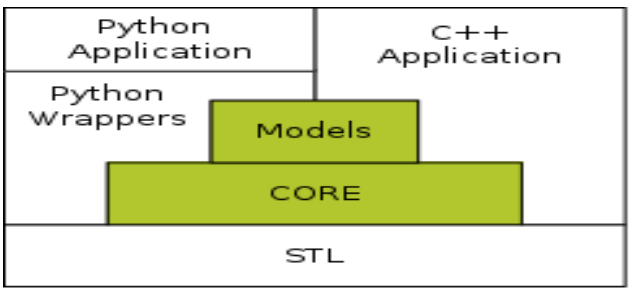
\includegraphics[width=5in]{figures/literature/ns3-architecture}
	\label{fig:ns3-architecture}
\end{figure}

\subsection{Robotics Simulator and Robotic Software}

Applications for physical robots can be created using robotics simulator without depending on the real hardware. This saves time and cost in the development of the application. Certain robotics simulator can render 3D model of robots and its environment, and can emulate robotic models, sensors, and control in virtual environment. They use physics engine to make the simulation more realistic.

\shortciteA{Staranowicz2011} has conducted a survey presenting comparison between the popular commercial and open-source robotic software for simulation and interfacing with real robots.  \shortciteA{Ivaldi2014} has conducted an online survey where participants present their feedback about the tools and use of dynamic simulation in robotics.

The most used robotics simulator are:
\begin{itemize}
	\item \textit{Gazebo.} Gazebo can simulate multiple robots in outdoor environments. It supports multiple physics engine. It can integrate with ROS using a set of ROS packages named gazebo\_ros\_pkgs. Gazebo is open source and free to use.
	\item \textit{ODE.} Open Dynamics Engine is a open-source physics library for simulating rigid body dynamics. It is used in computer games and simulation tools. It is open source.
	\item \textit{Bullet.} Bullet is an open-source physics library and is used in 3D animation software and game engines. It is open source.
	\item \textit{V-Rep.} V-Rep is a robot simulator software developed by Coppelia Robotics. It is free for academic usage. Commercial license is not free. 
	\item \textit{Webots.} Webots is an open-source robot simulator developed by Cyberbotics. It was open sourced in 2018. Robots can be modeled, programmed and simulated with the provided development environment.
\end{itemize}  

In this study, I intend to use Gazebo as the robotics simulator because:

\begin{itemize}
	\item The UAV firmware PixHawk provides SITL simulation for Gazebo and is the recommended option. 
	\item Gazebo supports PixHawk provided quad-copter (Iris).
	\item Gazebo supports multiple quad-copters.
	\item External world can be built in Gazebo using real world height maps.
	\item Gazebo supports sensors such as GPS and cameras.
	\item Gazebo can be integrated with ROS.
	\item Gazebo server provides API to integrate with other software. In my use case, I update the FANET nodes in ns-3 using the position provided by the robotics simulator. 
\end{itemize}

\section{Robot Operating System}
\shortciteA{Quigley2009} presents an overview of Robot Operating System (ROS). ROS is a framework for robotics software. It provides set of tools and communication layer on top of a host operating system, which helps in developing software for robotics. Availability of plethora of open source ROS packages avoids reinventing the wheel while developing the application.

ROS provides peer-to-peer connection to different processes of the robotics system. Each process is called a node and handles a specific aspect of the robotic system. The peer-to-peer topology makes use of a master node which enables the running nodes to find each other at run-time. Nodes exchange information with each other using messages. A message is a predefined strictly typed data structure. Nodes can exchange messages using either topic or service.

Nodes can publish message on a topic. Another node which uses the data generated by it can subscribe to the topic to receive messages. Nodes and topics have many-to-many association with each other. A single node can publish and subscribe to many topics and a topic may be published and subscribed by many nodes at once.

For synchronous communication, a node may call a service registered by another node. A node sends a request message to call a service and the node providing the service will reply with a response message. Unlike topics, service of a particular name can only be advertised by one node.

Nodes, topics and services can be grouped into namespaces. Topics and services follow URI reference naming convention. For example a topic that publishes GPS information for UAV 1 in a multi-UAV system may be named as \textit{/uav0/global\_position/gps}.

ROS has transformation system called tf/tf2. Tf2 is the new iteration of the transformation library. The transformation system helps the user keep track of multiple coordinate frames over time by using a tree structure to maintain relationship between coordinate frames. It allows for easy transformation of data between any two coordinate frames.

ROS has a wide array of tools for creating, debugging, inspecting and visualizing the data exchanged between the different nodes which speeds up the development.


\section{Multi-Agent Coverage Path Planning}

Coverage path planning (CPP) is the process of finding a suitable path that passes through a set of way-points in order to completely explore the area or volume of interest. The CCP problem is closely related to the lawnmower problem described by \shortciteA{Arkin2000}, and is proven to be NP-hard even for simple polygonal regions. Lawnmower problem is definded as finding a path/tour $\pi$ such that every point of the region $R$ is covered by some placement of the agent along $\pi$.

\shortciteA{Galceran2013}, on their survey of CPP methods mentions other closely related problems:

\begin{itemize}
	\item \textit{Covering salesman problem.} A generalization of the traveling salesman problem.
	\item \textit{Art gallery problem.} The minimum number of guards needed to station in a polygon area such that each point is visible to atleast one guard.
	\item \textit{Watchman route problem.} The shortest route in a polygon area such that each point is visible from the route.
\end{itemize}

All the above mentions problems are proven in general cases, to be NP-hard. Therefore, the solution to CPP problems are approximations to the problem.

Multiple agents can be helpful for the CPP task in many ways. Multiple agents can decrease the time taken to cover the area of interest and can be more robust as the exploration task can still be carried out if case of an agent failure. Multi-agent CPP is the process of finding a set of suitable paths through a set of way-points where the union of the found paths completely explore the area or volume of interest. 

\shortciteA{Almadhoun2019} has carried out an extensive survey for multi‑robot coverage path planning for model reconstruction and mapping. They classified the topics involved into:
\begin{itemize}
	\item Viewpoint generation,
	\item Coverage path planning approaches,
	\item Communication and task allocation, and
	\item Mapping.
\end{itemize}

Viewpoint generation can be generalized to generating potential way-points that can be used in coverage planning. Visiting all the  potential way-points will result in complete coverage of the area under scrutiny.

In another survey by \shortciteA{Xu2019}, which focuses on multi-agent coverage search, the topics have been classified as:
\begin{itemize}
	\item Environment modeling,
	\item Agent deployment, and
	\item Search Path Planning.
\end{itemize}

Environment modeling is a special case of viewpoint generation when the obstacles in the area to search is known beforehand. For unknown and dynamic environments, non-model based viewpoint generation is applied.

\subsection{Viewpoint Generation}

Viewpoint generation is the process of finding points or sub-regions in the area of interest. If all the viewpoints are visited by the participating agents, then complete coverage of the area is obtained. There are two methods in which viewpoints are generated, model based, and non-model based.

In model based viewpoint generation, prior information about the environment to survey is known.

In non-model based viewpoint generation, the next viewpoint is generated on the fly using real-time information about the environment.


\subsection{Coverage Path Planning Approaches}











\section{Structure from Motion}


\section{Chapter Summary}
All chapters except Chapter 1 must include an introductory paragraph/s and a chapter summary.

\FloatBarrier


    % set 0.5 inch indentation
\setlength{\parindent}{0.5in} 
% set paragraph space = 0 space
\setlength{\parskip}{0mm}
% set line space 1.5
\setlength{\baselineskip}{1.6em}

\chapter{METHODOLOGY}
\label{ch:methodology}

The different components of the proposed system and how they work together are described in this chapter.

\section{System Overview}
The system uses multiple drones with PixHawk flight controllers, each paired with an individual companion computer and a ground control station (GCS). The operator sets the origin of the global map and select a region of interest on the GCS using Mapviz, a ROS package. The system creates a grid over the region of interest and calculate paths for the drones. After the expected paths are calculated, the system calibrates the drones by finding an accurate transformation between each drone's local frame of reference and the global frame. To accomplish this, the drones move along a predefined flight path while the transformations between each drone's local map and the global map is refined. After calibration is complete, the system coordinates the flights of the drones as they move along the paths the system calculated, ensuring coverage of the region of interest. While flying their paths, the drones stream images from their cameras to the GCS. On the GCS, the SfM module receives the images and constructs an aerial map (a textured 3D mesh) with respect to the global map frame for the region of interest initially selected by the operator.


All the components runs on a single computer while simulating the system. In simulation mode, PX4 will be run in software in the loop (SITL) mode. Gazebo will be used to visualize the physical world and render simulated video feeds. Network Simulator 3 (NS3) will be used to simulate the networking functions of the wireless mesh network.

\section{System Design}

The different components comprising the system are described here.

\subsection{Components}

The system can be divided into two domains, one comprising the components in the drones, and the other comprising the components in the GCS. Components running on drones do not share information with other drones; they only share with the GCS. These components will be involved with vehicle platform manipulation and forwarding the images captured. The components on the GCS will be involved with getting the initial region of interest from the operator, planning the path of each drone, coordinating the movement of each drone during plan execution, requesting and receiving images from the drones, and aerial mapping from the images received.

The flight controller is installed with PX4 firmware. The companion computers and the GCS runs Ubuntu or Raspbian Linux with the Robot Operating System (ROS) installed and is connected to a wireless mesh network through IEEE 802.11 devices.

The components on the GCS are illustrated in Figure~\ref{fig:gcs-components} and as follows:
\begin{itemize}
	\item \textit{Computer.} An i7 laptop with 16 GB of RAM running Ubuntu 18 is the processing unit of the GCS.
	\item \textit{Wirless mesh router.}  Wireless mesh router provides mesh network to the laptop, as well as maintain mesh network with the drones.
	\item \textit{Robot Operating System.} All the components is designed and implemented with ROS as the base infrastructure. This gives access to the plethora of ROS tools and packages.
	\item \textit{mapviz.} Mapviz running as a plugin inside rqt is the GUI interface for the system. Mapviz is a ROS-based visualization tool with a plug-in system focused on visualization of 2D data. It shows tiled maps using the Microsoft Bing Maps API and has plugins to select polygons on the map, show markers, show NavSat data, among other features that fit the requirements of this system. Mapviz also allows us to fix the origin of the global map.
	\item \textit{image\_pipeline}. ROS image pipeline is used to rectify the image obtained from the cameras attached to the drones.
	\item \textit{pegasus\_planner.} A new multi-agent path planning ROS node designed for the project.
	\item \textit{pegasus\_controller.} A new ROS node that calculates and maintains translations between different map frames, monitor links with the drones, transmit path planning information to the drones, and coordinate the drones during flight.
	\item \textit{pegasus\_image\_subscriber.} A new ROS node that requests and receives images from the drones.
	\item \textit{pegasus\_image\_rectify.} A new ROS node that rectifies the received images for each individual drones' cameras using image\_pipeline.  
	\item \textit{Structure from Motion software.} An aerial map is constructed using the rectified images acquired from drones by this component. ODM (Open Drone Map) is used to build the map. ODM uses OpenSfM, an open source SfM software framework.
\end{itemize}

\begin{figure}
	\centering
	\caption[Pegasus system overview]{\small Architecture diagram of ground control station.}
	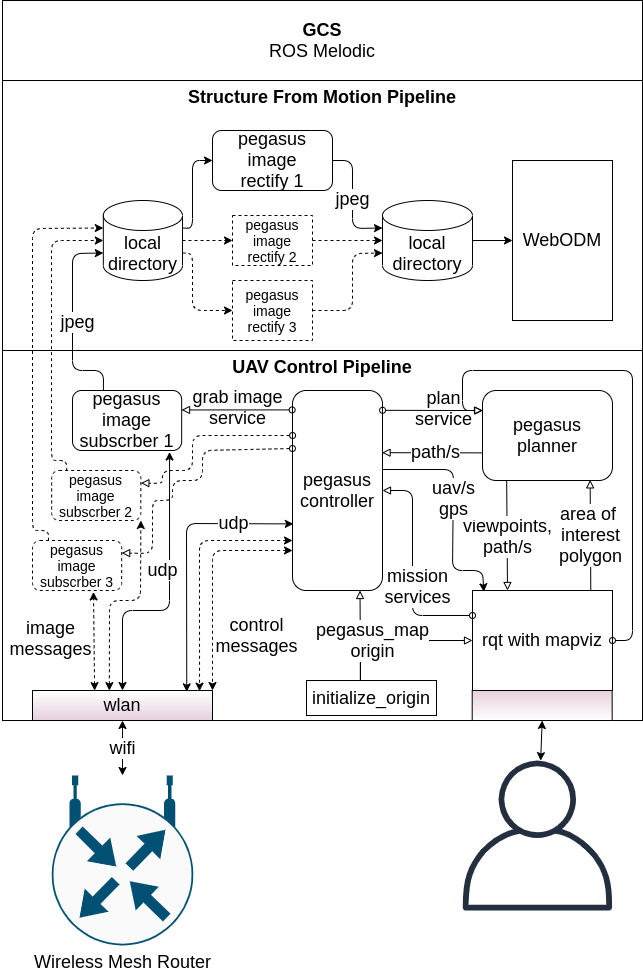
\includegraphics[width=5in]{figures/methodology/methodology-gcs-components}
	\label{fig:gcs-components}
\end{figure}

The components in the drones are illustrated in Figure~\ref{fig:drone-components} and as follows:
\begin{itemize}
	\item \textit{Flight Controller.} The drones will use Pixhawk flight controllers with PX4 as their firmware.
	\item \textit{Companion Computer.} The companion computer will control the flight controller in OFFBOARD mode through a serial link.
	\item \textit{Mobile wireless mesh router.} The mobile wireless mesh router will maintain mesh network using OSLR, and will provide network to the companion computer through ethernet link.
	\item \textit{USB camera.} The USB camera attached to the computer will enable the drone to capture images.
	\item \textit{Robot Operating System.} The software components will be designed and implemented as ROS nodes.
	\item \textit{mavros.} The companion computer will use mavros, a ROS package for MavLink communication between companion computers, and flight controllers, to control the flight controller in OFFBOARD.
	\item \textit{gscam.}  Gscam will be used to acquire video stream from the camera attached to the drone. Gscam is a ROS package which is based upon gstreamer.
	\item \textit{pegasus\_commander.} A new ROS node designed for the project that receives paths and control messages from the GCS. It will publish and subscribe to mavros for controlling, and receiving status of the drone. It will also send to the GCS, the drone's local poses, GPS positions, flight controller status updates, and GCS link monitoring information.
	\item \textit{pegasus\_image\_publisher.} The video feed from the onboard camera will be captured, geo-tagged with GPS information and sent to the GCS by this component.
\end{itemize}

\begin{figure}
	\centering
	\caption[Pegasus GCS system overview]{\small Architecture diagram of drone.}
	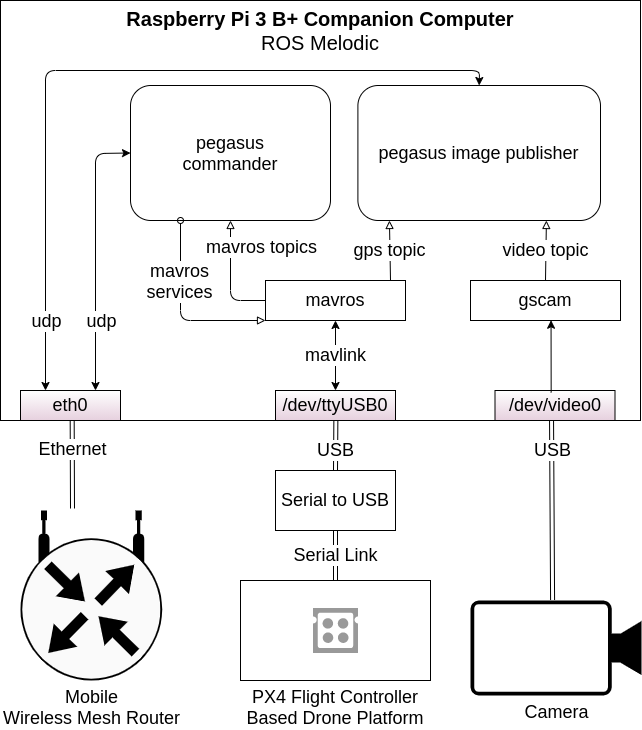
\includegraphics[width=5in]{figures/methodology/methodology-drone-components}
	\label{fig:drone-components}
\end{figure}


The operator will select the global map origin and region of interest through mapviz. The pegasus\_planner will create a grid-based representation of the region of interest and plan the paths for the drones in the global map reference frame.  The path planned by pegasus\_planner will be sent to pegasus\_controller. Pegasus\_controller will run a calibration routine on each of the drones to find the transformation between the local origin of the drone and the global map origin. These transformations allow the system to maintain the global map (pegasus\_map), where planning is carried out and the local map (uav0\_map, uav1\_map, etc.), where the control of the drones are achieved as shown in Figure~\ref{fig:map-heirarichy}. After calibration completes, pegasus\_controller will transform the paths for the drones from global map to the local map for each drone and send it to the drone. Pegasus\_controller will monitor the link with each drone by sending a periodic heart-beat packet. If a drone does not receive a heart-beat packet for some interval, it will change to Return To Home (RTL) mode and abort its current path. To avoid collision, pegasus\_controller will also maintain a path index counter. Paths are made up of a list of poses. Pegasus\_controller will tell each drone to move to the next pose in its path when all the drones have reached their current goal pose.

\begin{figure}
	\centering
	\caption[Different maps in pegasus system.]{\small Different maps in pegasus system.}
	
\includegraphics[width=5in]{figures/methodology/map-transformation-heirarichy}
	\label{fig:map-heirarichy}
\end{figure}


The drones will use mavros, which exposes MavLink protocol parameters and services as ROS topics and services. Pegasus\_commander will receive commands and path information from the GCS and execute its plan while sending local poses, global GPS positions, and flight controller state information back to the GCS. Gscam will publish video stream from the USB camera as a ROS camera topic. The pegasus\_image\_publisher will capture images from the published camera topic, apply GPS exif tag and send them to the GCS, as it receives request from pegasus\_image\_subscriber that will save the received images to a local directory. 

Pegasus\_rectify\_image will rectify the images using the camera calibration parameters, prepare the images for map building and save them to a directory in GCS . The SfM module will construct an aerial map for the region of interest selected by the operator from these images.


\subsection{Simulation}

Most of the components will remain the same regardless of whether running in simulation or in the real world. The simulation will run in a single computer. Four more components will be utilized to simulate the system:
\begin{itemize}
	\item \textit{Gazebo.} Gazebo simulator will be used because it supports fleet of drones and camera feed.
	\item \textit{PX4 Software in the loop.} PX4 firmware will be run as software in the loop, to simulate the drone's firmware. 
	\item \textit{pegasus-net-sim.} A custom network simulator 3 module that will simulate the mobility of the drones and push and pop actual control messages and video feed between the drones and the GCS through the simulator. It will also publish the SNR status of each device in the network.
	\item \textit{pegasus\_network\_status\_util\_node.} A custom ROS node that will receive noise and signal strength from pegasus-net-sim and publish the signal-to-noise ratio (SNR) value of each drone as ROS topic.
\end{itemize}


PX4 software in the loop (SITL) will be used to simulate the drone. PX4 SITL uses Gazebo to simulate the world, the drone mechanics and the video feed. Pegasus-net-sim, a Network Simulator 3 custom module will be used to simulate the wireless mesh network. Pegasus-net-sim will receive the model info from Gazebo and update the position of its nodes. Each node in pegasus-net-sim will have NS3PegasusApp, a custom NS3 application installed, which will send and receive packets in the simulated network. Pegasus-net-sim will function as a proxy application that will receive data in one UDP port, simulate it in NS3 and transmit it through another UDP socket. Using the trace feature in NS3, pegasus-net-sim will publish the noise and signal value for each node of the wireless mesh network.

Figure~\ref{fig:gcs-components-simulated} and Figure~\ref{fig:drone-components-simulated} illustrates the components used in simulation. 

\begin{figure}
	\centering
	\caption[Pegasus system simulaion overview]{\small Architecture diagram of simulated ground control station.}
	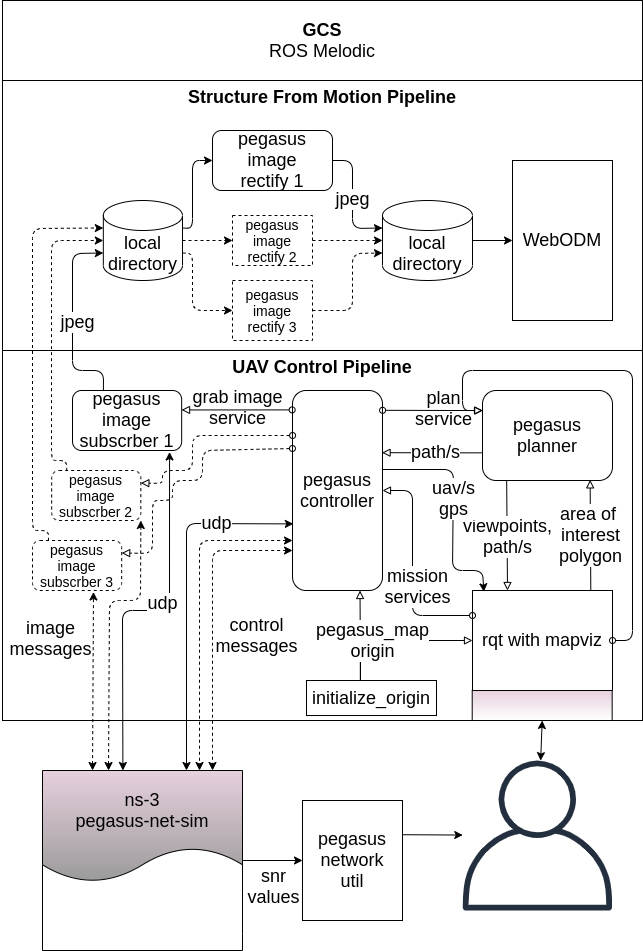
\includegraphics[width=5in]{figures/methodology/methodology-gcs-components-simulated}
	\label{fig:gcs-components-simulated}
\end{figure}
\begin{figure}
	\centering
	\caption[Pegasus GCS system simulation overview]{\small Architecture diagram of simulated drone.}
	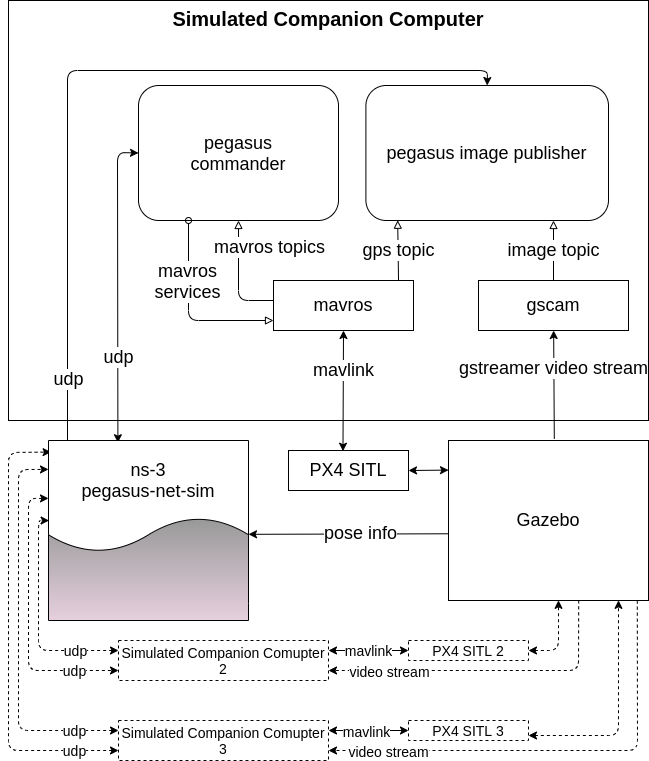
\includegraphics[width=5in]{figures/methodology/methodology-drone-components-simulated}
	\label{fig:drone-components-simulated}
\end{figure}


\subsubsection{pegasus-net-sim}

Network Simulator 3 is used to simulate wireless mesh network infrastructure. ns3 provides a framework to write simulations that can be integrated with other software. For this study ns3 should be able to:
\begin{itemize}
	\item Simulate a wireless mesh network with OLSR as the underlying mesh protocol to build the routing table for each node.
	\item Update the position of the nodes using the pose information from Gazebo. Gazebo library will be used to subscribe to gazebo pose topic.
	\item Inject and eject real world traffic between GCS and drones to the ns3 simulation. \texttt{pegasus-net-sim} will be designed as a proxy application between the components of the pegasus system to intercept traffic between them.
	\item Trace the signal noise value different nodes and publish it using the trace feature of ns3.
\end{itemize}

The architecture diagram of pegasus-net-sim is given in Figure~\ref{fig:pegasus-net-sim}. NS3PegasusDroneApp is a custom application for ns3 that will inject and eject the udp packets to and from the simulation. Each ns3 node will have a NS3PegasusDroneApp installed. A NS3PegasusDroneApp will have a set of PegassUDPSocket encapsulating real udp sockets and its virtual ns3 socket counterpart. Each PegasusUDPSocket class will have transmit and receive threads. These threads will continuously poll for any packet to send or receive in the real udp socket. PegasusUDPSocket will have a tx and rx lockless queue. Receive thread of a socket will write to the rx queue when it receives a packet. Transmit thread will poll the tx queue and transmit the packet to socket. NS3PegasusDroneApp running in ns3 simulation will poll the rx/tx queues of the PegasusUDPSocket in its set and inject/eject the packets to its virtual udp socket inside the simulation.

\begin{figure}
	\centering
	\caption[Architecture of \texttt{pegasus-net-sim}]{\small Architecture diagram of \texttt{pegasus-net-sim}.}
	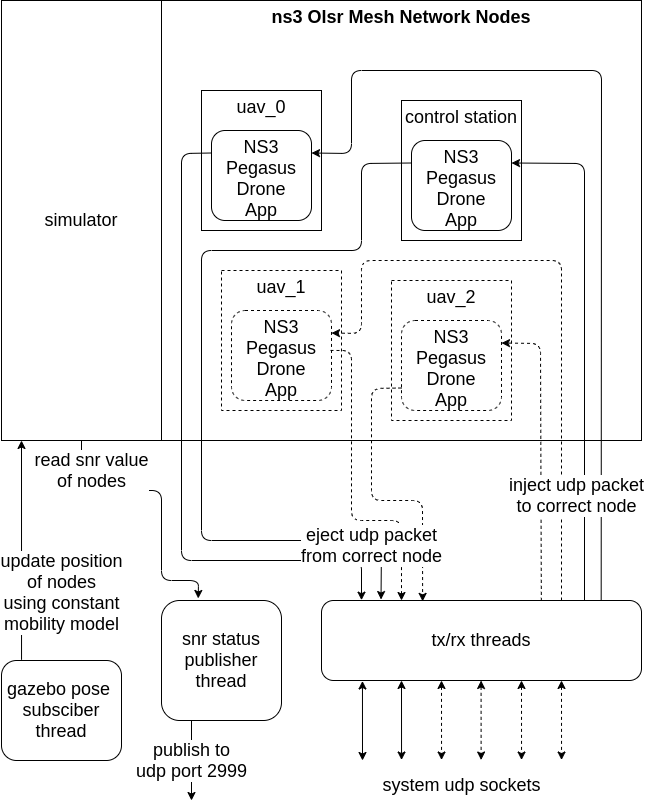
\includegraphics[width=5in]{figures/methodology/methodology-pegasus-net-sim}
	\label{fig:pegasus-net-sim}
\end{figure}

\begin{figure} 
	\centering
	\caption[Example of \texttt{pegasus-net-sim} intercepting packets.]{\small 
		A scenario with one GCS and two drone (a) Communication without network simulation (b) Communication packets being routed through \texttt{pegasus-net-sim}.}
	\subfloat[]{%
		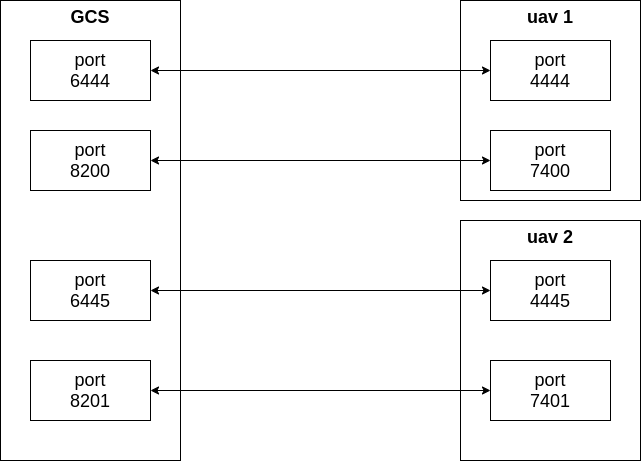
\includegraphics[width=5in]{figures/methodology/methodology-pegasus-net-sim-socket-binding}
	}
	
	\subfloat[]{%
		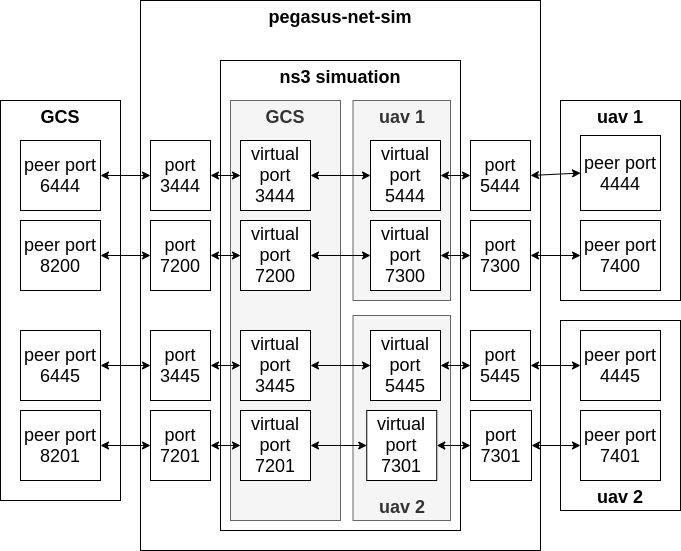
\includegraphics[width=5in]{figures/methodology/methodology-net-sim-routing}
	}
	\label{fig:pegasus-net-sim-simulation-example}
\end{figure}

To intercept and route a packet within pegasus-net-sim, it will have:
\begin{itemize}
	\item \textit{port.} The real udp port which will intercept real world traffic.
	\item \textit{virtual port.} The ns3 virtual port that will simulate port.
	\item \textit{peer port.} The real udp port which the port will transmit to.
	\item \textit{virtual peer port.} The ns3 virtual udp port that the traffic will get transmitted to.
\end{itemize}


Port and virtual port will have the exact same port number. For the configuration, three elements are defined in the tuple \{port, peer port, virtual peer port\}. For the scenario given in Figure~\ref{fig:pegasus-net-sim-simulation-example}, the corresponding configuration in PegasusConfig.cc will be:

\begin{verbatim}

std::map<std::string, std::vector<PegasusPortConfig>> 
PegasusConfig::m_config {
{
"iris_0", {
{5444, 4444, 3444},
{7300, 7400, 7200},
}
},
{
"iris_1", {
{5445, 4445, 3445},
{7301, 7401, 7201},
}
},
{
CONTROL_STATION_STR , {
{3444, 6444, 5444},
{7200, 8200, 7300},
{3445, 6445, 5445},
{7201, 8201, 7301},
}
},
};
\end{verbatim}

\subsection{pegasus\_network\_status\_util\_node}

The ns3 module pegasus-net-sim traces the signal and noise decibel of each packet of each node, smooths and averages it out per 100 millisecond per node and advertises it to udp port 2999. The pegasus\_network\_status\_util\_node reads the information on udp port 2999, and publishes signal to noise ratio (SNR) as ROS topics for each node for the user to analyses. 

\section{Functional Components}
The functional software components of the pegasus system can be categorized as:
\begin{itemize}
	\item \textit{Presentation.} This layer defines how the operator interacts with the system. Solely in the GCS.
	\item \textit{Planning.} This layer will calculate a list of grid based viewpoints and provide path through those viewpoints for the drones in the system, to cover the region of interest selected in the presentation layer. This layer will be in the GCS. 
	\item \textit{Motion control.} This layer will calculate the drones' local and global map transformations and control the motion of the drones according to path calculated in the planning layer. It will also align the drones in a particular direction at the viewpoints where it needs to capture an image and will request image acquisition service to acquire the image. This layer will be in the GCS as well as the drone.
	\item \textit{Image acquisition.}  This layer will be present in the GCS and the drone. It will provide service to capture image from the drone, apply GPS tags and deliver it to the GCS over the network. The images acquired will be saved in a local directory of the GCS.
	\item \textit{Map building.} After the drones have covered their paths, the map building layer will process the images in the local directory of the GCS.
\end{itemize}

\subsection{Presentation}

This layer presents how an end user will interact with the system. The front-end of the system will utilize a ROS package called mapviz. Mapviz will be used as a plugin inside ROS rqt. The ROS rqt will provide a dashboard for the operator to interact with. The GUI that the operator will be presented with is illustrated in Figure~\ref{fig:mapviz-screenshot}. The presentation layer will run in the GCS.

\begin{figure}
	\centering
	\caption[Pegasus presentation dashboard]{\small ROS rqt with mapviz visualizer. Origin for pegasus\_map is set near CSIM.}
	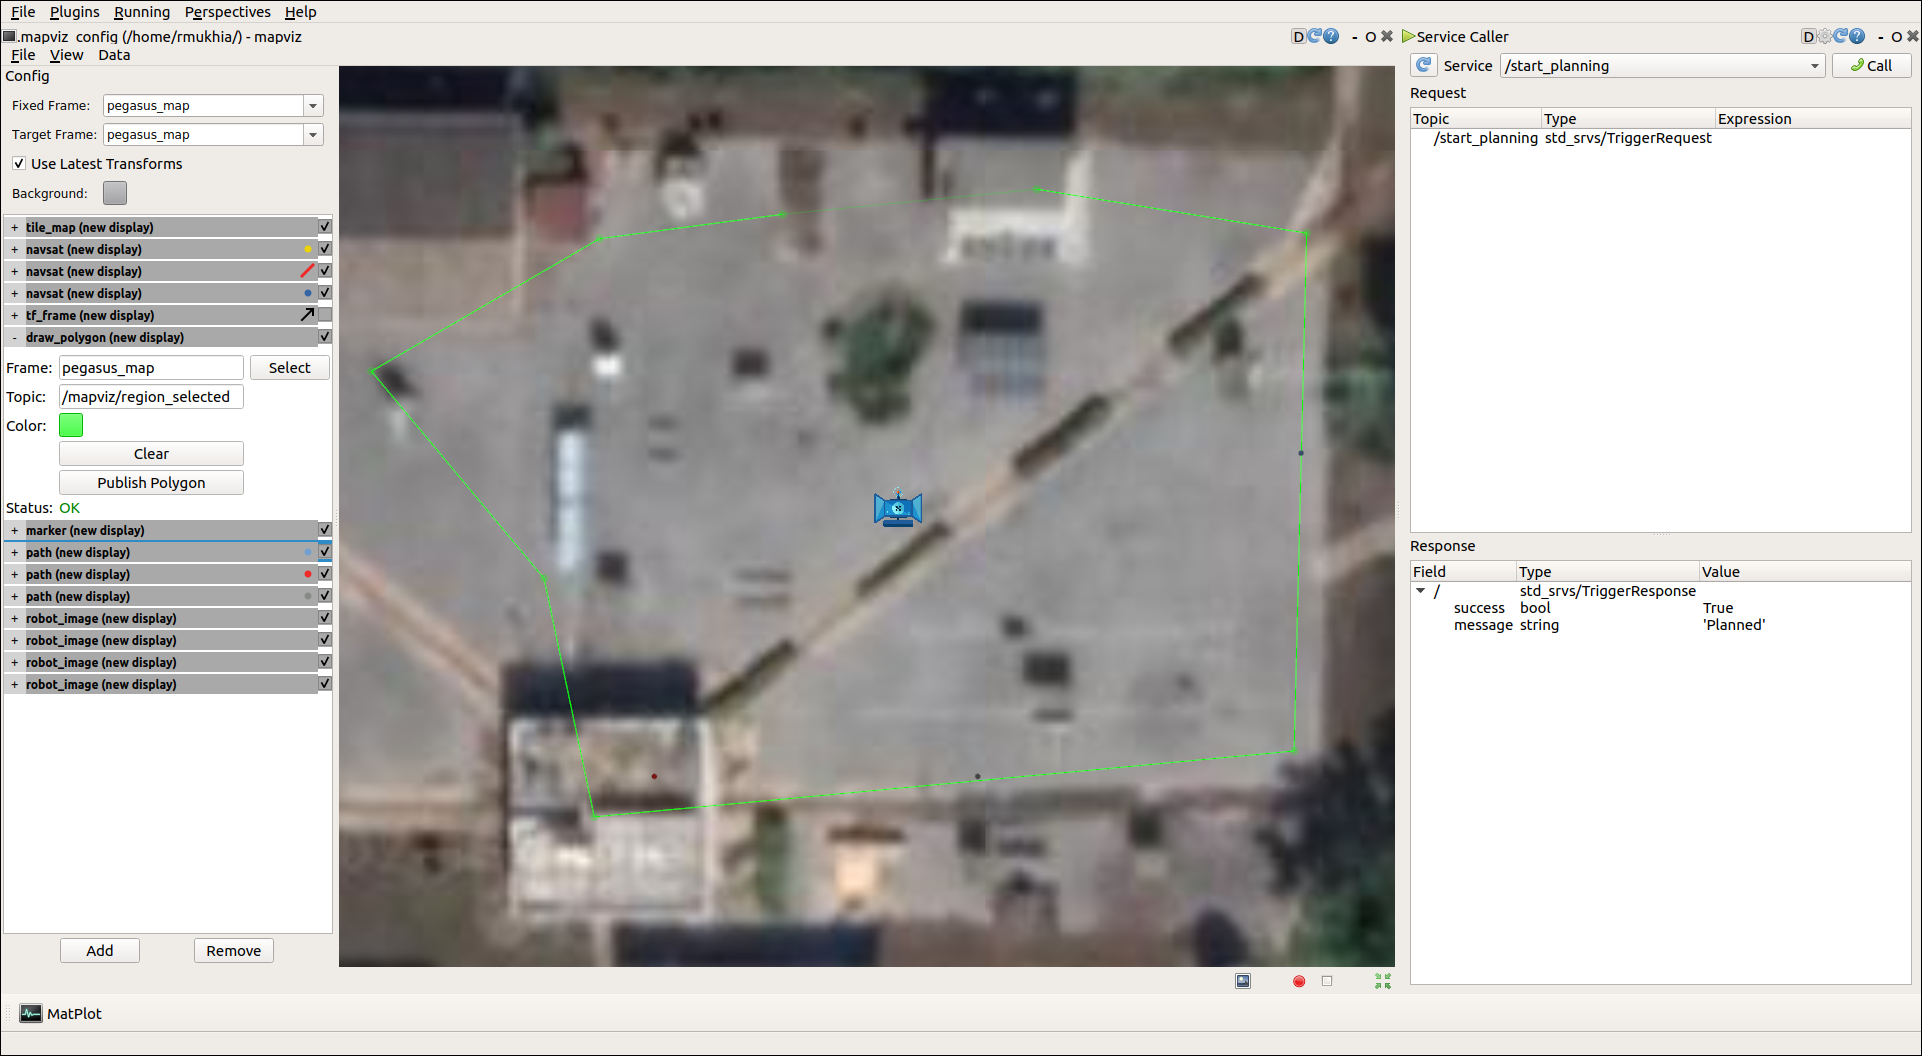
\includegraphics[width=5in]{figures/methodology/presentation/mapviz-1}
	\label{fig:mapviz-screenshot}
\end{figure}


\subsubsection{Mapviz}
Mapviz requires the operator to select the global map origin as a ROS parameter. ROS parameters can be set through the rosparams command-line tool, programmatically or in the launch file. In our case, we set the local map origin though the launch file using the ROS package swri\_transform\_util.


\begin{verbatim}
<?xml version="1.0"?>
<launch>
<node pkg="swri_transform_util" type="initialize_origin.py"
name="initialize_origin" >
<param name="local_xy_frame" value="/pegasus_map"/>
<param name="local_xy_origin" value="control_station"/>
<rosparam param="local_xy_origins">
[{ name: control_station,
latitude: 14.081104,
longitude: 100.612743,
altitude: 7,
heading: 0.0}]
</rosparam>
</node>
<node name = "pegasus_dashboard" pkg = "rqt_gui" type = "rqt_gui" 
respawn = "false" output = "screen" args = 
"--perspective-file $(find pegasus_ros)/pegasus_ros.perspective"/>
</launch>
\end{verbatim}


It will publish two ROS topics:
\begin{itemize}
	\item /local\_xy\_origin: Origin of the global map.
	\item /mapviz/region\_selected: The points of the polygon as selected by the user.
\end{itemize}

The mapviz module can use online map APIs such as google maps and bing maps. For offline use, mapproxy can be used to cache data locally and serve it to mapviz. \textit{https://github.com/danielsnider/MapViz-Tile-Map-Google-Maps-Satellite} provides a docker image for mapproxy that integrates well with mapviz.

The flow that the operator has to follow while using this GUI is presented in Figure~\ref{fig:presentation-flow}.

\begin{figure}
	\centering
	\caption[Operator interaction with pegasus system]{\small A flowchart of the operator's interaction with the presentation layer.}
	
\includegraphics[width=5in]{figures/methodology/presentation/presentation-flow}
	\label{fig:presentation-flow}
\end{figure}


\begin{figure}
	\centering
	\caption[Operator interaction with pegasus system; a scenerio.]{\small 
		A scenario where an operator (a) Selects an area of interest (b) Publishes the polygon (c) Calls start\_planning service.}
	\subfloat[]{%
		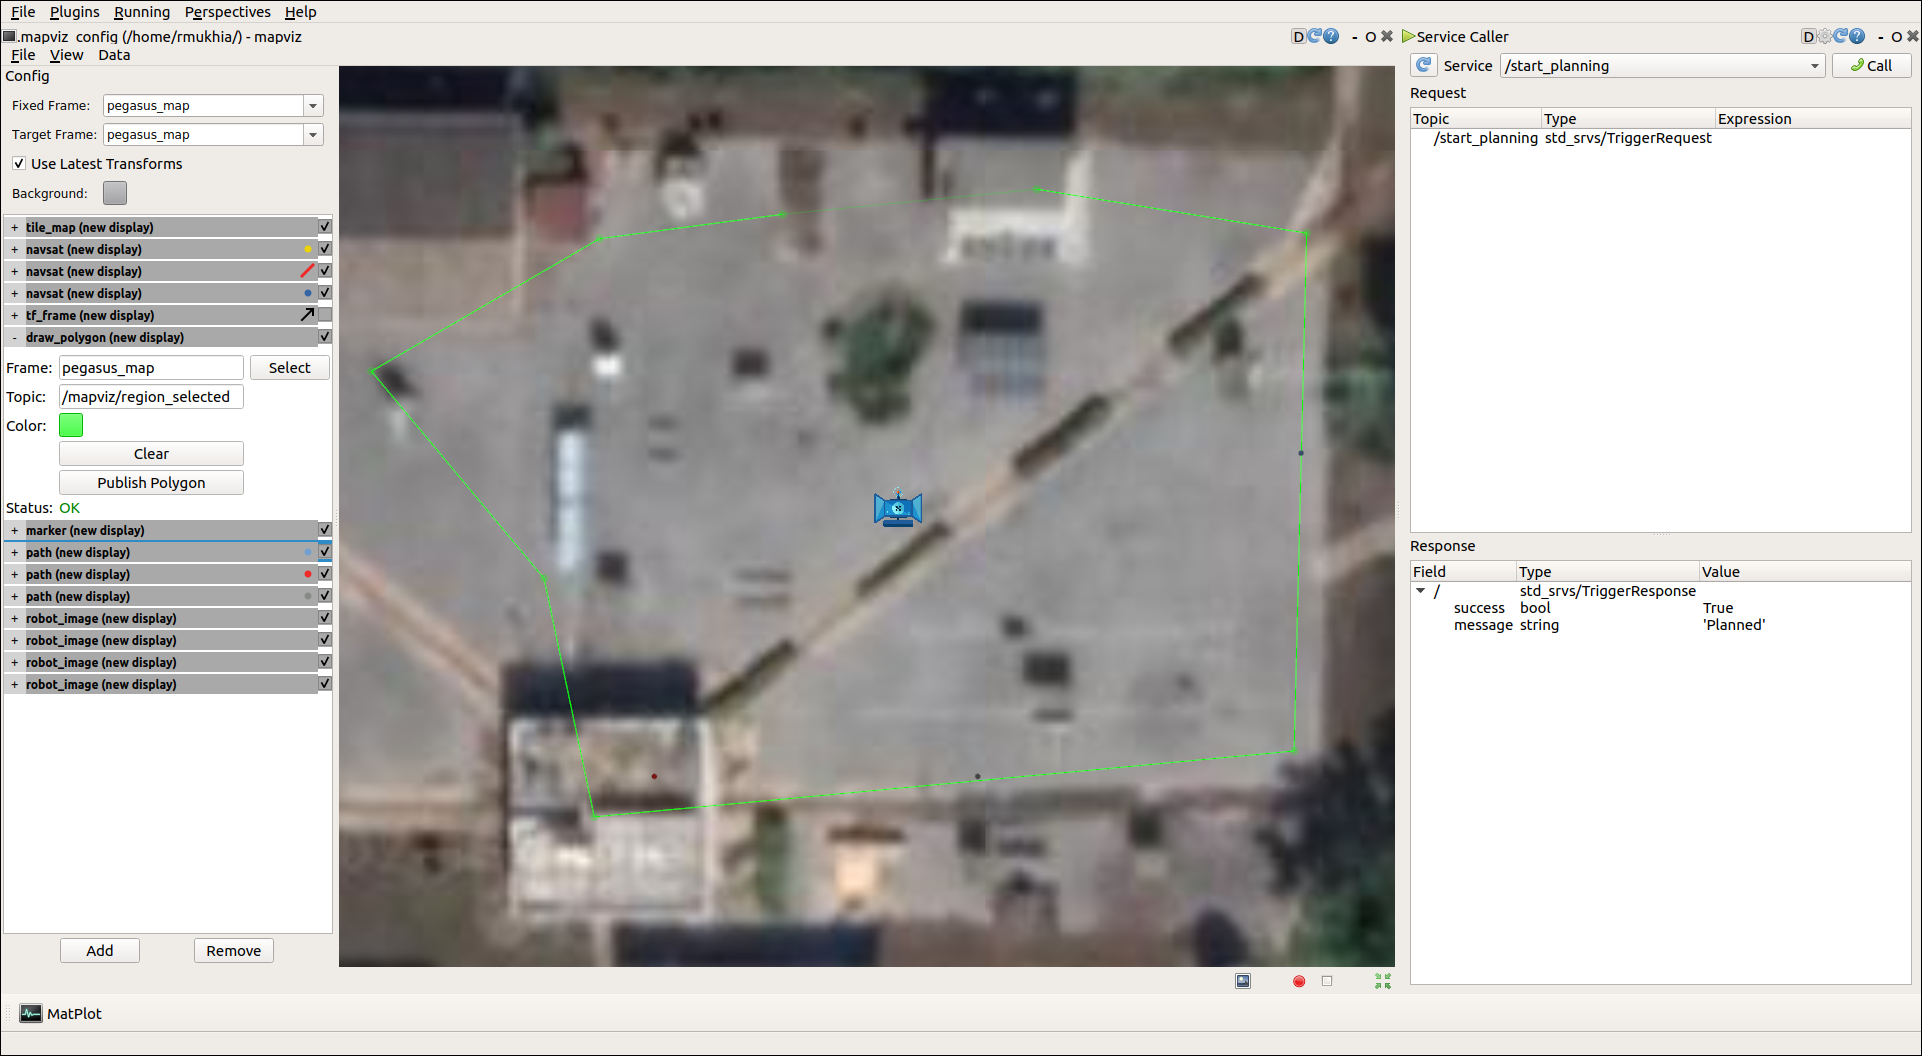
\includegraphics[width=4in]{figures/methodology/presentation/mapviz-1}%
	}
	
	
	\subfloat[]{%
		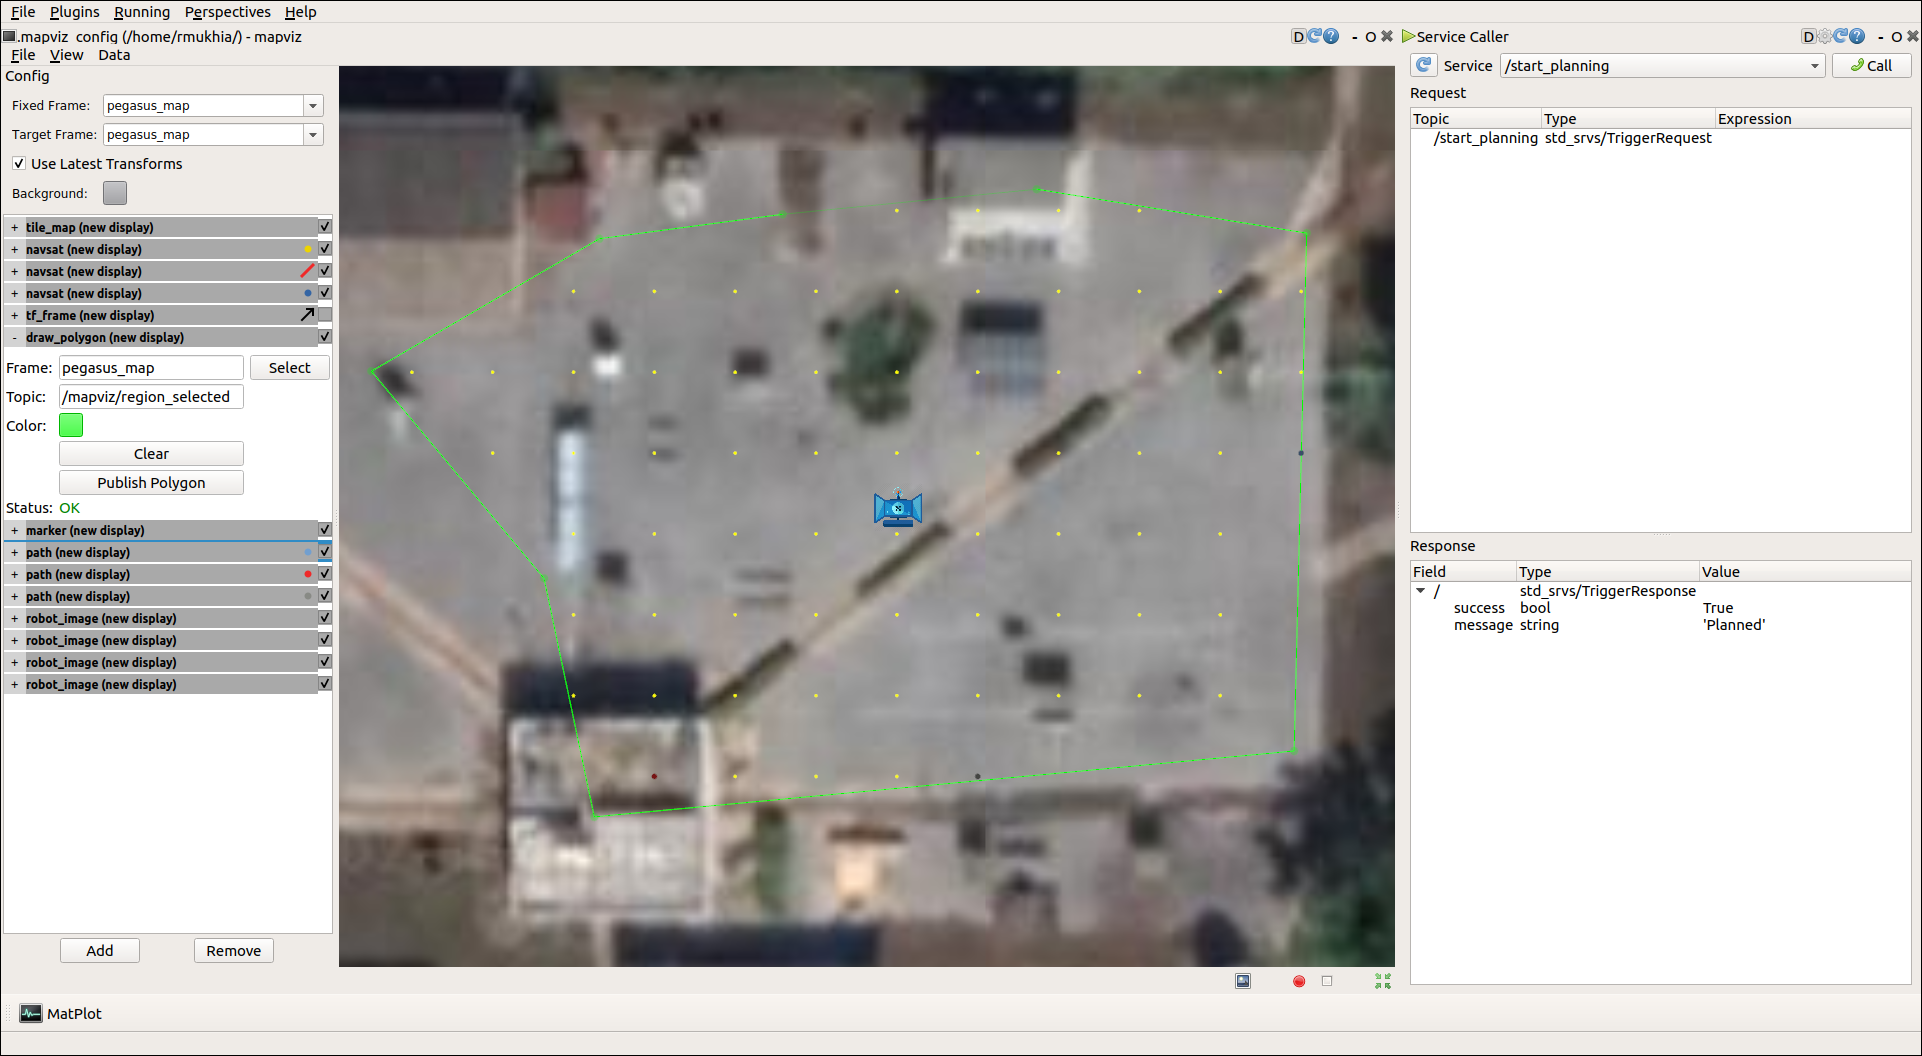
\includegraphics[width=4in]{figures/methodology/presentation/mapviz-2}
	}
	
	
	\subfloat[]{%
		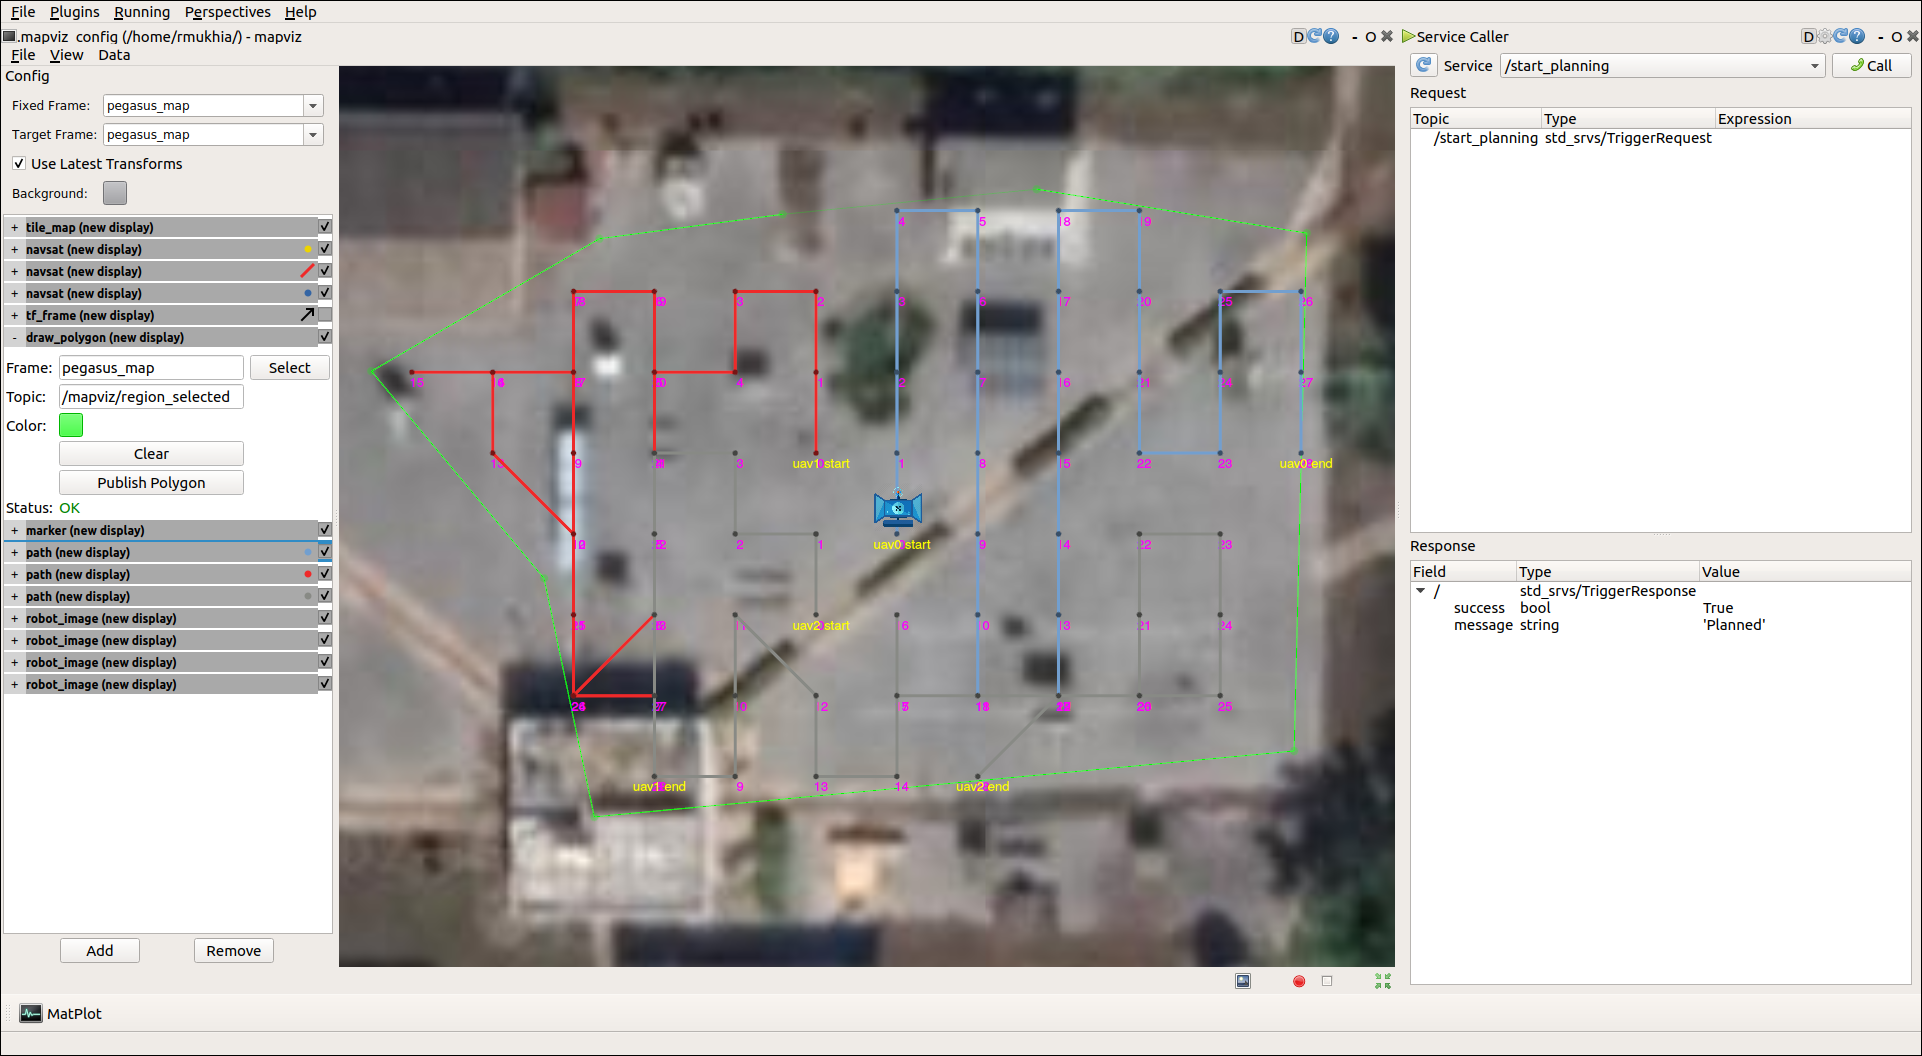
\includegraphics[width=4in]{figures/methodology/presentation/mapviz-3}
	}
	
	\label{fig:presentation-scenerio-1}
\end{figure}


\subsection{Planning}

This layer will compute the path for the drones which will cover the region of interest selected by the operator. It has one component, the pegasus\_planner.

\subsubsection{Pegasus\_planner}

Pegasus\_planner will handle the following tasks:
\begin{itemize}
	\item \textit{Viewpoint generation. } Generate grid cells based viewpoint in the region of interest.
	\item \textit{Multi-agent coverage path planning. } A* search to calculate the optimal paths for each drone, such that they avoid collisions and stay within the constraints of the wireless mesh network in the global map frame.
\end{itemize}

\textbf{Viewpoint Generation}

To generate a valid grid inside the region of interest, consider a polygon with $n$ vertices:

\begin{figure}
	\centering
	\caption[Structure of control messages.]{\small 
		The steps in viewpoint generation (a) Polygon showing the area of interest. (b) Bounding box on the Polygon showing the area of interest. (c) Bottom left position of the cells in the bounding box. (d) Rays projecting from cell centre to $x_{max} + 1$. (e)  Grid cells inside the region of interest. }
	\subfloat[]{%
		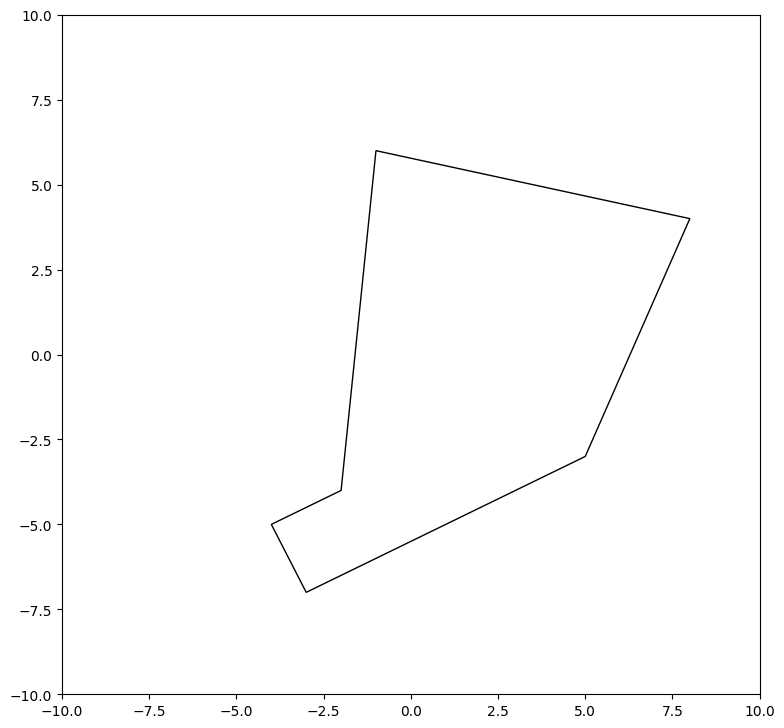
\includegraphics[width=.4\textwidth]{figures/methodology/pegasus_planner/generate_grid/polygon}%
	}
	\subfloat[]{%
		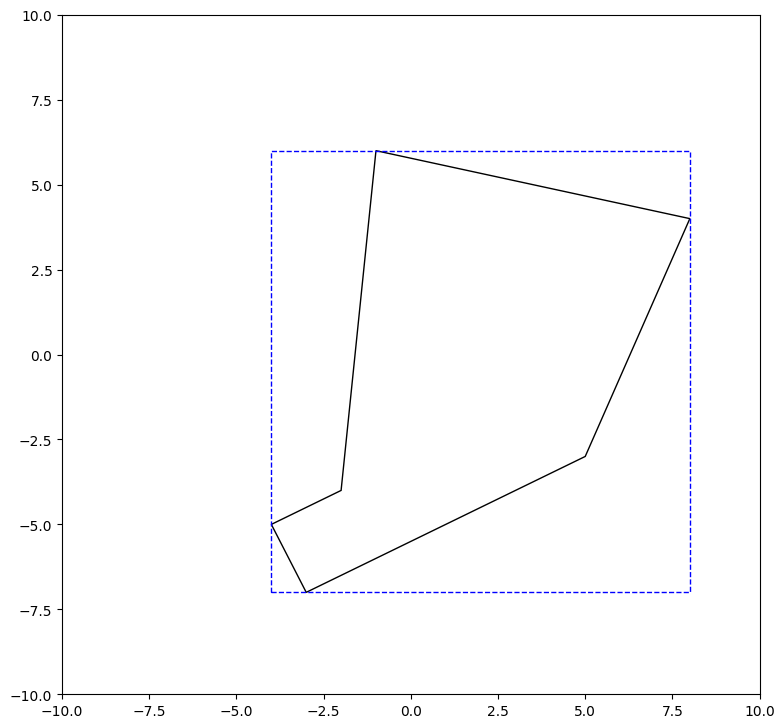
\includegraphics[width=.4\textwidth]{figures/methodology/pegasus_planner/generate_grid/bounding-box}
	}
	
	
	\subfloat[]{%
		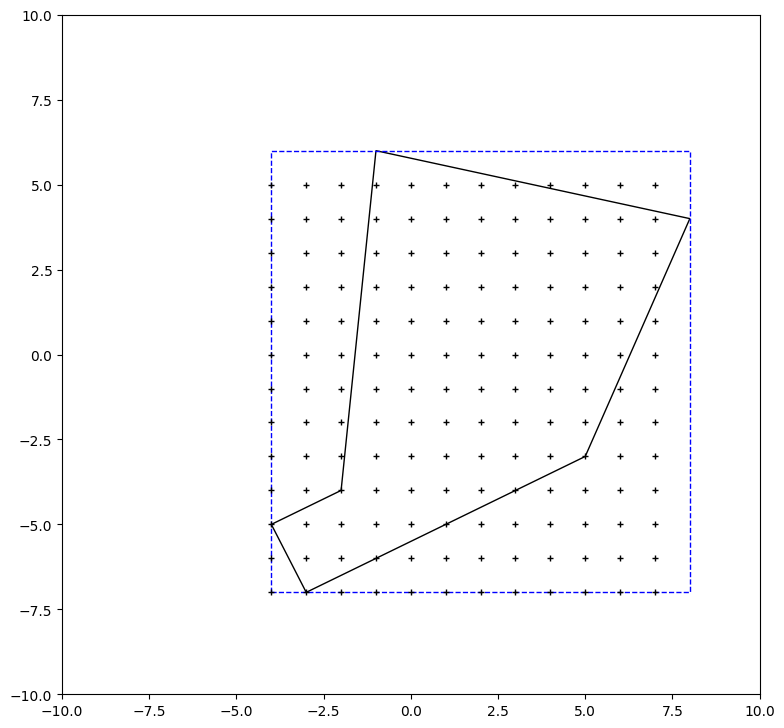
\includegraphics[width=.4\textwidth]{figures/methodology/pegasus_planner/generate_grid/cells}%
	}
	\subfloat[]{%
		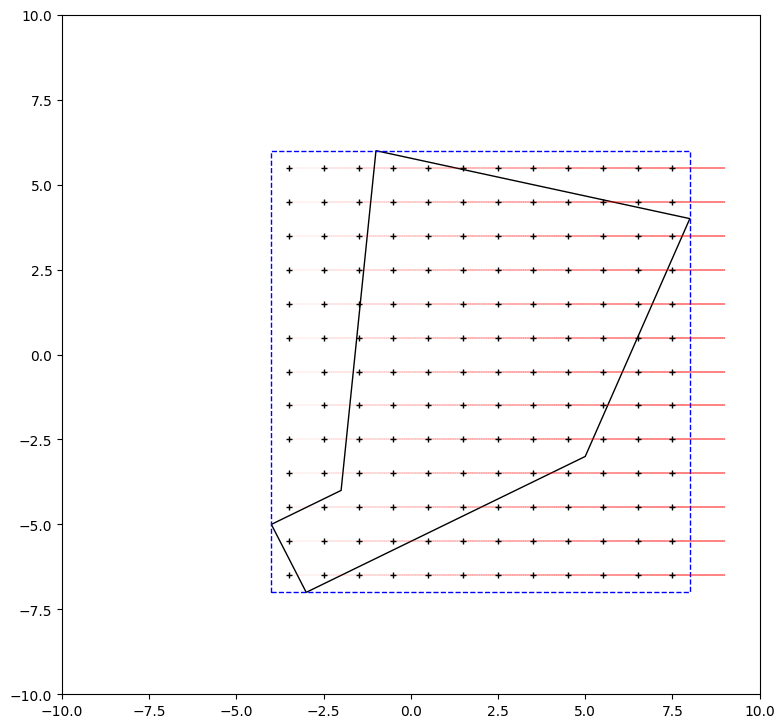
\includegraphics[width=.4\textwidth]{figures/methodology/pegasus_planner/generate_grid/ray}
	}
	
	\subfloat[]{%
		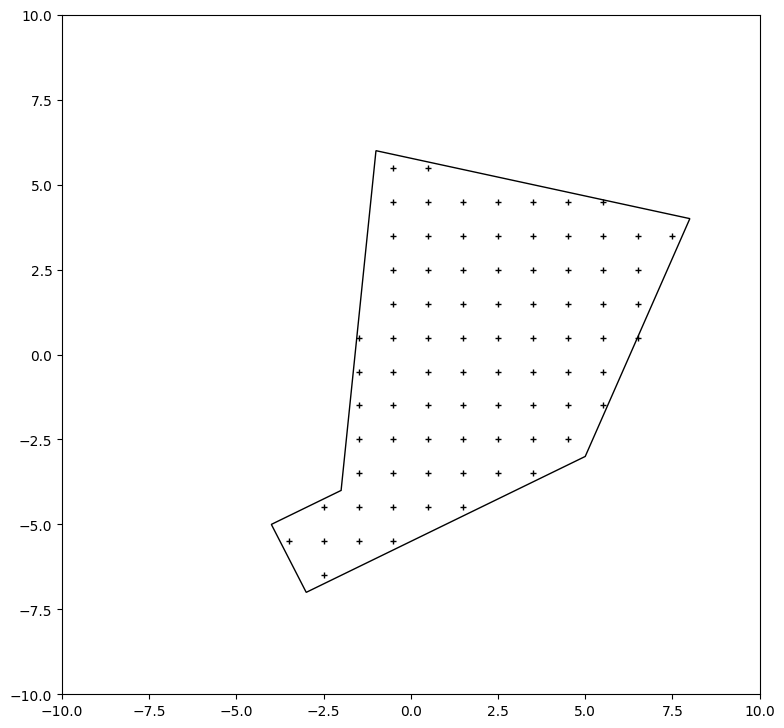
\includegraphics[width=.4\textwidth]{figures/methodology/pegasus_planner/generate_grid/valid-cells}
	}
	
	\label{fig:viewpoint-generation}
\end{figure}

$$
\text{polygon} = \begin{bmatrix}
x^0 & y^0 \\
x^1 & y^1 \\
x^3 & y^2 \\
\vdots  & \vdots \\
x^{n-1} & y^{n-1} \\
\end{bmatrix}. 
$$

The vertices are arranged counter-clockwise/clockwise. To find the bounding box of the polygon, we need to find the vertices.

$$
\text{boundingBox} = \begin{bmatrix}
x_{min} & y_{min} \\
x_{max} & y_{min} \\
x_{max} & y_{max} \\
x_{min} & y_{max}
\end{bmatrix},
$$



where each row defines a vertex. Consider a grid with $n$ cells either horizontally or vertically. Let $c$ be the grid cell size.

$$c = \text{BoundingBox}_{width|heigh} \div  n $$

Alternatively, we can set a fixed size for each cell, or calculate the cell size from camera parameters and the altitude of the drone.

We can then calculate the coordinates $(b^{i,j}_x, b^{i,j}_y)$ of the bottom left vertex of each cell.

$$\text{cells} =\begin{bmatrix}
b^{0,0}_x & b^{0,0}_y \\
b^{1,0}_x & b^{1,0}_y \\
b^{2,0}_x & b^{2,0}_y \\
\vdots & \vdots \\
b^{i_{max} - 1,0}_x & b^{i_{max} - 1,0}_y \\
b^{0,1}_x & b^{0,1}_y \\
b^{1,1}_x & b^{1,1}_y \\
b^{2,1}_x & b^{2,1}_y \\
\vdots & \vdots \\
b^{i_{max} - 1,0}_x & b^{i_{max} - 1,0}_y \\
\vdots & \vdots \\
b^{i_{max} - 1,j_{max}-1}_x & b^{i_{max} - 1,j_{max} - 1}_y \\
\end{bmatrix}$$

$$b^{i,j}_x = x_{min} + i * c$$
$$b^{i,j}_y = y_{min} + j * c$$

$i$, $j$ are the index in $x$  and $y$ axis respectively.


We can get the range of $i$ and $j$ as follows.
$$i_{max} = \left\lceil\frac{x_{max} - x_{min}}{c}\right\rceil $$
$$j_{max} = \left\lceil\frac{y_{max} - y_{min}}{c}\right\rceil$$

Let the number of vertices in $gridCells$ be $k$:
$$ k = i_{max} \times j_{max}.$$


We can then calculate grid index $(i,j)$ from $[0, k]$:

$$j = \left\lfloor\frac{k}{i_{max}}\right\rfloor$$
$$i = k  - j \times i_{max}.$$



Since the vertex $v$ of the polygon is arranged counter-clockwise/clockwise, we can easily get the vertices of line segment for each side of the polygon.

$$v_i = (x_i, y_i)$$
$$s < n$$

$$\text{polygonLineSegments}=\begin{bmatrix}
v_0 & v_1 \\
v_1 & v_2 \\
\vdots & \vdots \\
v_s & v_{s+1} \\
\vdots & \vdots \\
v_{s_{max}-1} & s_0 \\
\end{bmatrix}$$

$$=\begin{bmatrix}
x_0 & y_0 & x_1 & y_1 \\
x_1 & y_1 & x_2 & y_2\\
\vdots && \vdots \\
x_s & y_s & x_{s+1} & y_{s+1} \\
\vdots && \vdots \\
x_{n-1} & y_{n-1} & x_{0} & y_{0} \\
\end{bmatrix}$$

We can imagine that the center of each grid cell projects a line parallel to the $x$ axis till $x_{max} + 1$.

$$\text{cellCenter} = [\text{cells}] +  \frac{c}{2}$$
$$\text{rays} = \begin{bmatrix}
\text{cellCenter}_x^{0,0} & \text{cellCenter}_y^{0,1} & x_{max} + 1 & \text{cellCenter}_y^{0,1} \\
\text{cellCenter}_x^{1,0} & \text{cellCenter}_y^{1,1} & x_{max} + 1 & \text{cellCenter}_y^{1,1} \\
\text{cellCenter}_x^{2,0} & \text{cellCenter}_y^{2,1} & x_{max} + 1 & \text{cellCenter}_y^{2,1} \\
\vdots && \vdots \\
\text{cellCenter}_x^{k-1,0} & \text{cellCenter}_y^{k-1,1} & x_{max} + 1 & \text{cellCenter}_y^{k-1,1} \\
\end{bmatrix}
$$


Now we apply ray tracing to check if $cell^{i,j}$ is inside our polygon or not. We count how many intersections each $rays^{i,j}$ makes with all the lines in $polygonLineSegments$. If the number of intersections are even, then the $cell$ is outside the polygon. If the number of intersections are odd, then the $cell$ is inside the polygon. We now have the valid cells that can the drones can traverse.


\textbf{Multi-agent Coverage Path Planning}

Considering a set of cells  $C$ for an area of interest with $n$ agents.  Multi-agent coverage path planning should compute coverage paths $p_i$ for each $ith$ agent where $p_i \subset C$ and  $\bigcup\limits_{i=1}^{n} p_i \subseteq C$. If $\bigcup\limits_{i=1}^{n} p_i = C$, then complete coverage is obtained.

We use A* search to find $p_i$ in $C$ for each agent. Let the set of search space in the A* search space be denoted as $S$, which is a tree with root node $s_0$.

A* search uses the cost function
$$ f = g + h $$

Where $g_k$ is the total cost till the current state $s_k$ and $h_k$ is the heuristic cost till the goal state $s_\text{goal}$ from $s_k$. $k$ is the id of nodes in the search tree.


There are 8 directions an agent can move to:
\begin{enumerate}
	\item Right
	\item Right-Top
	\item Top
	\item Left-Top
	\item Left
	\item Left-Bottom
	\item Bottom
	\item Right-Bottom
\end{enumerate}


In our case in each state progression a single agent moves in one direction, in round-robin fashion.  For example, if there are 3 agents, in state $s_l$ agent 1 may move left, in state $s_{l+1}$ agent 2 may move right, in state $s_{l+2}$ agent 3 may move  bottom, in state $s_{l+3}$ agent 1 may move top, and so on.

Let us define $g_k$ and $h_k$ for our setup. Let $m_k$ be the movement cost of agents to reach state $s_k$ from previous state $s_{k-1}$.

$$ m_k = 1, \text{if agent reaches an unvisited cell}. $$
$$ m_k = m_{prev} \times 2, \text{if agent reaches a visited cell, with previous movement cost } m_{prev} $$

Therefore, $\sum\limits_{k=0}^k m_k$ is the sum of all movement cost for agents to reach $s_k$ from $s_0$.

$$g_k = \sum\limits_{k=0}^k m_k $$

$$ h_k = \text{unvisited cells in } C$$


Therefore, a state $s_k$ will have:
\begin{itemize}
	\item $m_k$. The immediate movements to reach $s_k$.
	\item $g_k$. All movements for all agents to reach state $s_k$.
	\item $h_k$. Unvisited cell at $s_k$.
	\item $O_k$. Set of cells that the agents are occupying in the state $s_k$.
	\item $V_k$. Visited cells with recorded movement costs. To compute $h_k$ for the state.
\end{itemize}

$$ s_k = \{m_k, g_k, h_k, O_k, V_k\} $$

We must define equality operation for the state for A* to work.

$$ s_\sigma = s_\theta, \iff O_\sigma = O_\theta $$


The other parameters we need to set for our A* algorithm are:
\begin{itemize}
	\item \textit{MAX\_DISTANCE.} The max range of mesh client. 
	\item \textit{CS\_POSITION.} The position of control station in global map.
	\item \textit{Z\_HEIGHT.} The operational height of agents.
\end{itemize}


The constraints for A* search are:
\begin{itemize}
	\item At least one agent must move.
	\item The euclidean distance between any two pair of agents should not be greater than MAX\_DISTANCE.
	\item At least one agent should have euclidean distance with CS\_POSITION less than or equal to MAX\_DISTANCE.
	\item Any two agents cannot swap position. $$\begin{matrix} \label{eq:swap_agent}
	A & B && \to && B & A\\
	0 & 0 && && 0 & 0
	\end{matrix} \\
	$$
	
	\item Any two agents path line equation must not intersect between the previous cell and present cell. $$
	\begin{matrix} \label{eq:intersect_agent}
	A & 0 && \to && 0 & B\\
	B & 0 &&&& 0 & A
	\end{matrix}
	$$
\end{itemize}

Running A* using these parameters computes paths $p_i$, with $\bigcup\limits_{i=1}^{n} p_i = C$. However, it is not efficient as A* is not an approximation algorithm but an exhaustive search algorithm, and the problem we are trying to solve is NP-hard.


Branching factor for each node of our search tree is 8. However, the depth of the search tree increases as we add more agents. Therefore, the number of cells and agents drastically increases our running time. To decrease this,we will not compute the optimal steps to the end step, but we will lookahead certain number of steps, and progressively step ahead. This way we may not get the optimal solution, but the computing time will be saved. 

We will progressively reach our goal state through iterations of A* algorithm. For each A* iteration, we will stop the search by:
\begin{itemize}
	\item \textit{Depth Exit.} The depth exit mechanism will return $d$ number of decision $D$, that is it will travel $d+1$ depth in the search space and return the $D_d$ decision set. 
	\item \textit{Early Exit.} If we do not minimize the cost $f$ for  $\epsilon$ number of nodes, we will do early exit.
	
\end{itemize}

If the optimal decisions is $o$, the agent will take $q$ number of $d$ decision, where the cost will be

$$o \le \Sigma_{i=0}^q D^{0-d}_i$$

Also, if the heuristics does not improve for $\sigma$ A* iterations, then the search will stop.

$$ if, D^{0-d}_i == D^{0-d}_{i+1}, \forall \space 0 \le i < \sigma - 1; \text{stop}$$

The resulting decision list may have trailing states which have the same $h$. This is inconvenient for us and does not contribute to our problem, so we will trim the decision to the least $h$

\subsection{Motion Control}

This layer handles the control of drones through the ground control station. It will have the components, pegasus\_controller in the GCS, and pegasus\_commander, mavros and PX4 in the drone. A single pegasus\_controller will send requests to each drone's pegasus\_commander. The structure of response and reply messages are illustrated in Figure~\ref{fig:control-messages}. 
The different control messages that will be received by pegasus\_commander from pegasus\_controller are:
\begin{itemize}
	\item \textit{HEART\_BEAT.} Heart beat in regular intervals. This message is the only type to which pegasus\_commander will respond.
	\item \textit{SET\_OFFBOARD.} Put the flight controller in off-board mode.
	\item \textit{SET\_RETURN\_TO\_HOME.} Put the flight controller in return mode.
	\item \textit{SET\_ARM.} Arm the flight controller.
	\item \textit{GOTO(pose). } Move to drone to pose position.
\end{itemize}

\begin{figure}
	\centering
	\caption[Structure of control messages.]{\small 
		Structure of control messages between \texttt{pegasus\_controller} and \texttt{pegasus\_commander} (a) Request Message (b) Response message.}
	\subfloat[]{%
		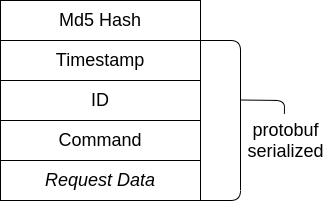
\includegraphics[width=.5\textwidth]{figures/methodology/methodology-request-message}%
	}
	\subfloat[]{%
		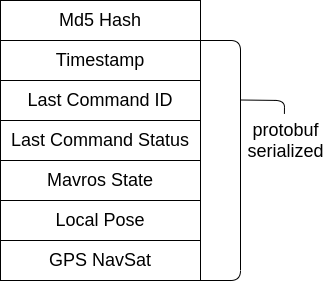
\includegraphics[width=.5\textwidth]{figures/methodology/methodology-response-message}
	}
	
	\label{fig:control-messages}
\end{figure}

HEART\_BEAT will have command id 0. SET\_OFFBOARD, SET\_RETURN\_TO\_HOME, SET\_ARM, and GOTO will have incremental id. That is for every new command, the id will increment by one. HEART\_BEAT reply will have the last command id received by pegasus\_commander and the status of its execution. Last command status is set to true when the command has been executed. Figure~\ref{fig:communitation-controller-commander} illustrates the communication between one pegasus\_controller and two pegasus\_commander.

\begin{figure}
	\centering
	\caption[Communication between \texttt{pegasus\_controller} and two \texttt{pegasus\_commander}.]{\small GOTO command communication diagram between \texttt{pegasus\_controller} and two \texttt{pegasus\_commander}.}
	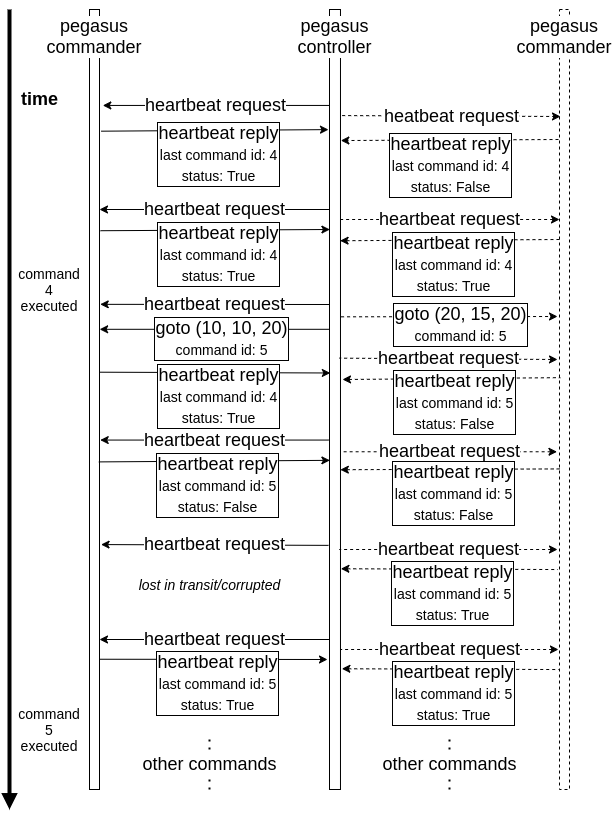
\includegraphics[width=5in]{figures/methodology/methodology-commander-controller-communication}
	\label{fig:communitation-controller-commander}
\end{figure}

\subsubsection{Pegasus\_controller}

Pegasus\_controller will be responsible for:
\begin{itemize}
	\item Calculating and maintaining the transformations between the local map frames of each drone and the global map frame.
	\item Coordinating and sending control messages to the drones.
	\item Monitoring the link with the drones by sending heart beat control message.
	\item Publishing local pose, global GPS coordinates and state of each drone, received in the heart beat reply as ROS topics.
	\item Calling image acquisition service to acquire images from the drones.
\end{itemize}

\begin{figure}
	\centering
	\caption[Architecture of \texttt{pegasus\_controller}.]{\small Architecture of \texttt{pegasus\_controller}.}
	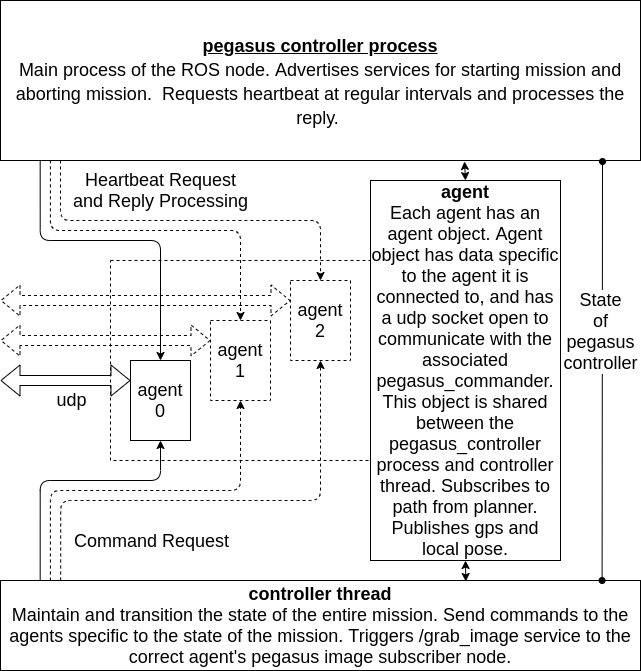
\includegraphics[width=5in]{figures/methodology/methodology-pegasus-controller}
	\label{fig:pegasus-controller}
\end{figure}

The architecture diagram of pegasus\_controller is given in Figure~\ref{fig:pegasus-controller}.
\begin{figure}
	\centering
	\caption[State diagram of \texttt{pegasus\_controller}.]{\small State diagram of \texttt{pegasus\_controller}.}
	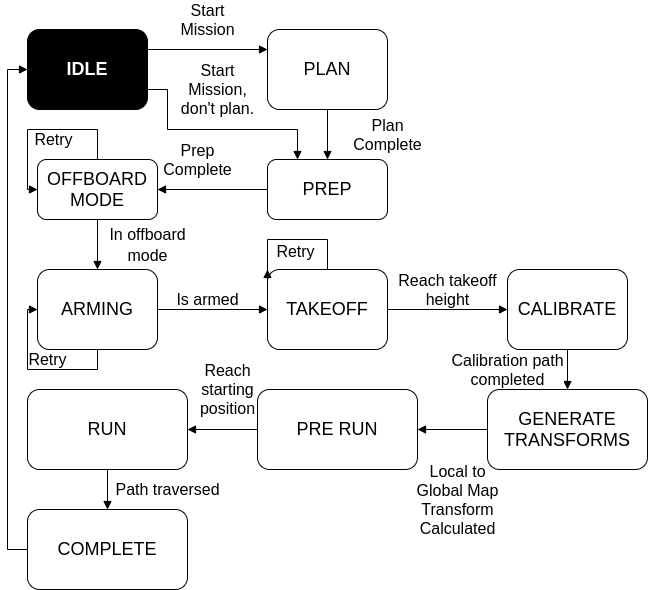
\includegraphics[width=5in]{figures/methodology/methodology-controller-state-diagram}
	\label{fig:controller-state-diagram}
\end{figure}

The state diagram in Figure~\ref{fig:controller-state-diagram} can be further elaborated as follows:
\begin{itemize}
	\item \textit{IDLE.} It will not do anything.
	\item \textit{PLAN.} Call services provided by pegasus\_planner. 
	\item \textit{PREP.} Prepare the drone to enter offboard mode.
	\item \textit{OFFBOARD\_MODE.} It will send SET\_OFFBOARD control message to the drones and wait for confirmation.
	\item \textit{ARMING.} It will send SET\_ARM control message to the drones and wait for confirmation.
	\item \textit{TAKE\_OFF.} It will takeoff drones to operational height.
	\item \textit{CALIBRATE.} It will send the calibration path to the drones and coordinate the flight of the drone along the calibration path and capture the corresponding local poses and global GPS positions for calculation the map transformations.
	\item \textit{GENERATE\_TRANSFORMS.} It will generate the transforms between the local map frame of each drone and the global map frame using the corresponding points collected in CALIBRATE state.
	\item \textit{PRE\_RUN.} Move the drones to starting position.
	\item \textit{RUN.} It will execute path of the drones in a coordinated manner.
	\item \textit{COMPLETE.} It will reach this state when the system's execution is complete. Set the drone to Return mode by sending SET\_RETURN\_TO\_HOME control message.
\end{itemize}

The drone will takeoff in its home position. After it reaches its operational height, it will follow a predefined routine from CALIBRATE state to PRE\_RUN state as shown in Figure~\ref{fig:calibration-routine}.  All the drones will be positioned at the origin of the global map (pegasus\_map) at different altitudes in PRE\_RUN state. For a mission with operational height $z_o$ and $n$ drones, the $i^{th}$ drone, were $0 <= i < n$ will have $z = z_o + i * 2$ meters altitude in PRE\_RUN state. 

\begin{figure}
	\centering
	\caption[Predefined routine before the start of the coordinated path traversal]{\small Predefined routine before the start of the coordinated path traversal. Steps 1-4 will be executed in CALIBRATE state, step 5 will be executed in PRE\_RUN state, and in step 6 the drone will move to the first pose in the planned path.} 
	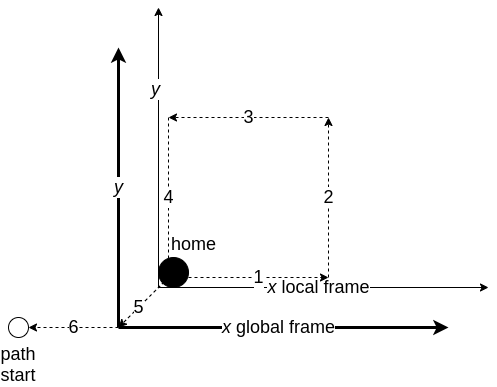
\includegraphics[width=5in]{figures/methodology/methodology-calibration-routine}
	\label{fig:calibration-routine}
\end{figure}

In GENERATE\_TRANSFORM state , algorithm~\ref{alg:find-transforms} will be used to find transforms between local map of each drone and the global map. The problem of finding transforms between all the local and global maps can be done with planar homography because the z axis of all the maps are parallel and pointing upwards.

In RUN state,pegasus\_commander will be configurable to allow two types of movement:
\begin{itemize}
	\item \textit{Towards.} The drones will face toward the direction it is moving. During image acquisition the drones will orient itself by setting their yaw to 0\degree as shown in Figure~\ref{fig:towards-movement}.
	\item \textit{Strafe.} The drones will always have its yaw at 0\degree. They will move sideways to the next viewpoint. This movement requires less time when the viewpoints are separated by small distances. Figure~\ref{fig:strafe-movement} shows this movement.
\end{itemize}

\begin{figure}
	\centering
	\caption[Movement types for drones.]{\small 
		Drones will be able to be configured to follow either (a) Towards movement, or  (b) Strafe movement. Towards movement takes more time than strafe movement because it has to know whether it has reached the destination pose in step 5, and if it has properly aligned to take image in step 6. In strafe movement the drone is already aligned to take image and it just needs to know wheather it has reached the destination pose in step 4. }
	\subfloat[]{%
		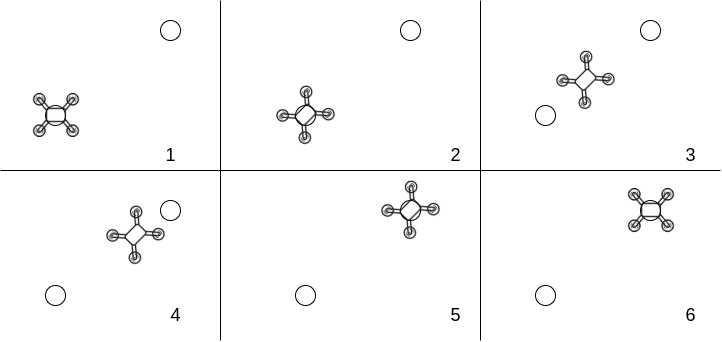
\includegraphics[width=5in]{figures/methodology/methodology-towards-movement}%
		\label{fig:towards-movement}
	}
	
	
	\subfloat[]{%
		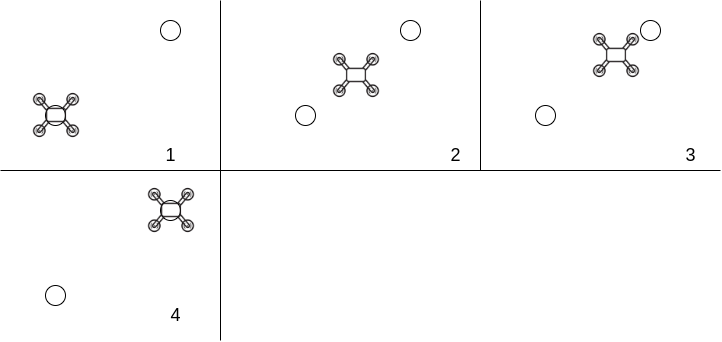
\includegraphics[width=5in]{figures/methodology/methodology-strife-movement}
		\label{fig:strafe-movement}
	}
	\label{fig:movement-types}
\end{figure}

Image acquisition will be skipped if the drone has already visited the viewpoint to avoid duplicate images.

\renewcommand{\algorithmicrequire}{\textbf{Input:}}
\renewcommand{\algorithmicensure}{\textbf{Output:}}
\renewcommand{\algorithmicforall}{\textbf{for each}}
\begin{algorithm}
	\caption{Find Local To Global Transformation}
	\label{alg:find-transforms}
	\begin{algorithmic}
		\REQUIRE $L$: set of all corresponding local poses
		\REQUIRE $G$: set of all corresponding global GPS positions
		\REQUIRE $O$: global map origin GPS coordinate
		\ENSURE $T$: transformation between local and global map
		\STATE $\widetilde{O} \gets \textsc{Convert-to-UTM}(O)$
		\STATE $\widetilde{G} \gets \textsc{Convert-to-UTM}(G)$
		\STATE $M \gets \widetilde{G} - \widetilde{O}$
		\STATE $\widehat{M} \gets \textsc{Remove-Z-axis}(\widetilde{M})$
		\STATE $\widehat{L} \gets \textsc{Remove-Z-axis}(L)$
		\STATE $H \gets \textsc{Find-Homography}(\widehat{L}, \widehat{M}, \text{RANSAC})$
		\STATE $T \gets \begin{bmatrix}
		H_{1,1} & H_{2,1} & 0 & H_{3,1} \\
		H_{1,2} & H_{2,2} & 0 & H_{3,2} \\
		0 & 0 & 1 & 0 \\
		0 & 0 & 0 & 1
		\end{bmatrix}$
		
	\end{algorithmic}
\end{algorithm}

In COMPLETE state, the drones will return to their home position following the behavior defined in PX4 firmware. PX4 firmware ascends the drone to a safe altitude before returning them to home. To avoid collision, the drones' safe altitude should be set different from each other.

\subsubsection{Pegasus\_commander} \label{section:pegasus-commander}

Pegasus\_commander is a new ROS node, customized for this study that will use the topics and services provided by mavros to control the drone in off-board mode. It will receive control messages from the pegasus\_controller. It will also monitor the link between GCS and the drone, and if a HEART\_BEAT control message is not received for a particular duration, then the flight controller will be set to Return mode. The architecture diagram of this module is shown in Figure~\ref{fig:pegasus-commander}.
It will only respond to HEART\_BEAT control message with:
\begin{itemize}
	\item The last command id it received and the status of the command,
	\item State of mavros,
	\item Local Pose of the drone in the local map,
	\item GPS coordinates of the drone.
\end{itemize}

For SET\_ARM, SET\_OFFBOARD and SET\_RETURN\_TO\_HOME it calls the relevant mavros services. For GOTO, it publishes the pose it received to mavros until it reaches the desired pose. Algorithem ~\ref{alg:is-at-position} will be used to determine if the drone has reached the desired pose.

\renewcommand{\algorithmicrequire}{\textbf{Input:}}
\renewcommand{\algorithmicensure}{\textbf{Output:}}
\renewcommand{\algorithmicforall}{\textbf{for each}}
\begin{algorithm}
	\caption{Is at position.}
	\label{alg:is-at-position}
	\begin{algorithmic}
		\REQUIRE $P_e$: expected pose 
		\REQUIRE $P_a$: actual pose
		\REQUIRE $d$: offset distance
		\REQUIRE $y$: offset yaw
		\ENSURE $A$: Boolean True or False 
		\STATE $D \gets |\textsc{euclidean\_distance}(P_e.position, P_a.position)|$
		\STATE $Y_e \gets \textsc{get\_yaw\_from\_quaternion}(P_e.orientation) $
		\STATE $Y_a \gets \textsc{get\_yaw\_from\_quaternion}(P_a.orientation) $
		\STATE $Y \gets |Y_e - Y_a|$
		\STATE $A \gets (D < d) \land (Y < y)$
	\end{algorithmic}
\end{algorithm}

\begin{figure}
	\centering
	\caption[Architecture diagram of\texttt{ pegasus\_commander}.]{\small Architecture diagram of \texttt{pegasus\_commander}.} 
	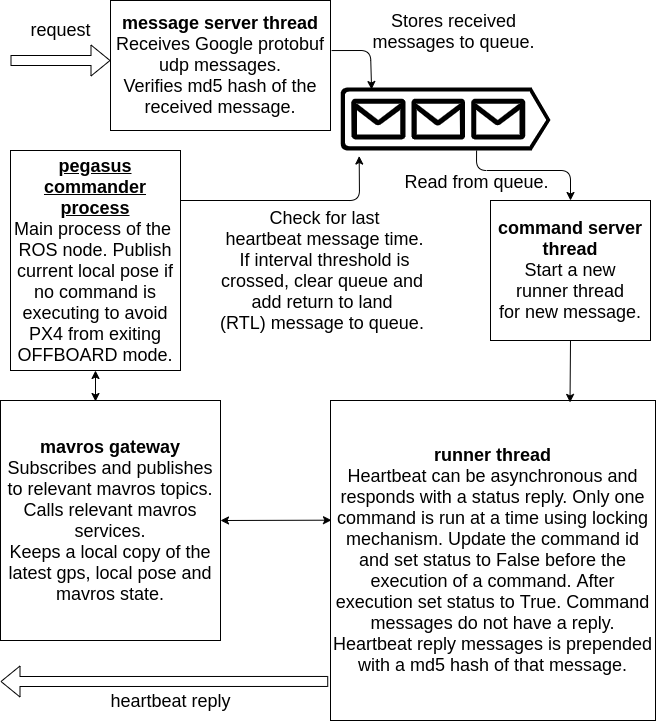
\includegraphics[width=5in]{figures/methodology/methodology-pegasus-commander}
	\label{fig:pegasus-commander}
\end{figure}

\subsubsection{PX4}
The drone runs PX4 Firmware on the flight controller. The flight controller's movement and altitude can be controlled in Offboard mode through the MAVlink protocol. This mode supports only a very limited set of MAVLink commands.

MAVLink commands supported in Offboard modes are:
\begin{itemize}
	\item SET\_POSITION\_TARGET\_LOCAL\_NED: Control vehicle position.
	\item SET\_ATTITUDE\_TARGET: Control vehicle altitude and orientation.
\end{itemize}

PX4 supports the coordinate frames (coordinate\_frame field): MAV\_FRAME\_LOCAL\_NED and MAV\_FRAME\_BODY\_NED.

A stream of setpoint commands must be received by the vehicle prior to engaging the mode, and in order to remain in the mode (if the message rate falls below 2Hz the vehicle will stop). In order to hold position while in this mode, the vehicle must receive a stream of setpoints for the current position.

Offboard mode requires an active connection to a remote MAVLink system (e.g. companion computer or GCS). If the connection is lost, after a timeout (COM\_OF\_LOSS\_T) the vehicle will attempt to land or perform some other failsafe action. The action is defined in the parameters COM\_OBL\_ACT and COM\_OBL\_RC\_ACT which can be set through mavros' mavparam.

\subsubsection{Mavros}

Mavros is a ROS node that provides ROS interfaces for communication with various autopilots with MAVLink communication protocol.
The ROS services provided by Mavros,  of interest for this system are:
\begin{itemize}
	\item \textit{mavros/set\_mode.} Required to set mode of the flight controller to off-board mode and return to launch mode.
	\item \textit{mavros/cmd/arming.} Required to arm the flight controller.
\end{itemize}

The ROS topics published by Mavros, useful for this system are:
\begin{itemize}
	\item \textit{mavros/state.} Publishes the state of the flight controller.
	\item \textit{mavros/local\_position/pose.} Publishes pose, i.e. position and orientation of the flight controller in the local frame. Mavros handles the translation between NED and ENU conventions.
	\item \textit{mavros/global\_position/global.} Publishes the GPS coordinates, i.e. latitude, longitude and altitude of the flight controller.
\end{itemize}

The ROS topics subscribed by Mavros, that this system will use are:
\begin{itemize}
	\item \textit{mavros/setpoint\_position/local.} Set the pose, i.e. position and orientation that the flight controller is desired to achieve in local frame.
\end{itemize}


\subsection{Image Acquisition}

This layer provides image acquisition service. The GCS will be able to request geo-tagged image from the drone in flight, using image acquisition service. The software components in this layer are gscam and pegasus\_image\_publisher in the drones and pegasus\_image\_subscriber in the GCS. The gscam ROS node is used to publish camera video feed as ROS camera topic using gstreamer. Mavros is used to acquire GPS location of the image captured. The pegasus\_image\_subscriber will provide a ROS service in the GCS which is called by pegasus\_controller to acquire images at the viewpoints. The pegasus\_image\_subscriber will be a udp client that requests image from the pegasus\_image\_publisher udp server in the drone. For multiple drones there will be multiple pegasus\_image\_subscriber running under different ROS namespace in the GCS. The subscriber and the publisher will transfer data with each other using the packet as shown in Figure~\ref{fig:image-packet}.

\begin{figure}
	\centering
	\caption[Packet structure for image acquisition.]{\small Packet structure for image acquisition.} 
	\label{fig:image-packet}
	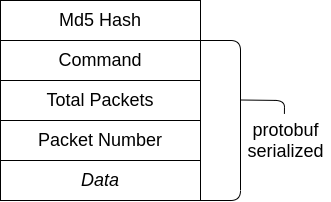
\includegraphics[width=3in]{figures/methodology/methodology-Image-packet}
\end{figure}

The same packet structure will be used by both the subscriber and publisher, however the commands are different for each:
\begin{itemize}
	\item \textit{REQUEST.} This request will be sent from subscriber to the publisher. The publisher will drop the previous buffer, capture a new image, add GPS tag to it, segment the image into multiple packets and store in buffer.
	\item \textit{REPLY.} The publisher will respond to the subscriber for the REQUEST packet. It will have the total packets in the buffer for the image requested.
	\item \textit{PKT.} The subscriber will request image packets from the publisher using the packet number it wants. It will request the same packet number until it receives the packet and then increment the packet number. The publisher will fill the data section with the image data and reply. The request will be made till the packet number reaches the total packets received in REPLY.
	\item \textit{ERR.} If the publisher cannot find the packet number the subscriber is requesting for, it will respond with ERR message.
\end{itemize}

The communication diagram is illustrated in Figure~\ref{fig:image-communication-diagram}.

\begin{figure}
	\centering
	\caption[Communication diagram for image acquisition.]{\small Communication diagram for image acquisition.} 
	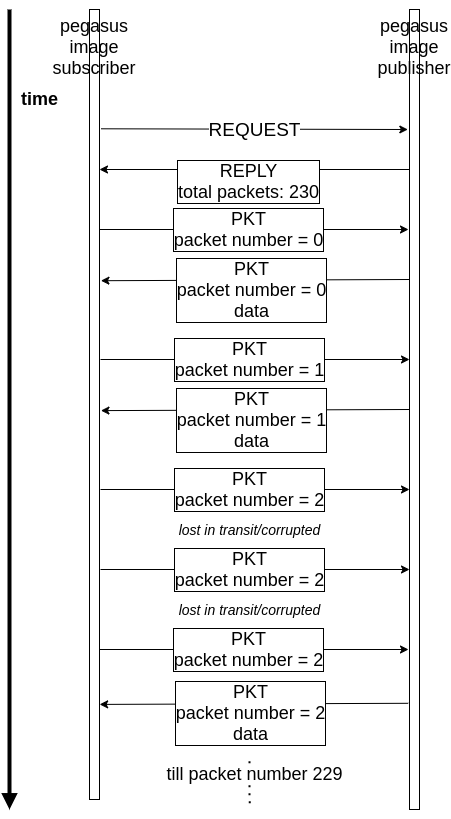
\includegraphics[width=4in]{figures/methodology/methodology-image-communication-diagram}
	\label{fig:image-communication-diagram}
\end{figure}


\subsubsection{Pegasus\_image\_publisher}

The gscam ROS node will provide the USB camera video feed as ROS topic. The pegasus\_image\_publisher node will subscribe to the ROS camera topic and GPS topic published by mavros. When it receives a REQUEST message from the pegasus\_image\_subscriber, it will get the current video frame and gps data, and store GPS data using Exchangeable Image File (EXIF) format. It will store the geo-tagged image in buffer till a new REQUEST message is received. It will provide image data to the subscriber from the current buffer.


\subsubsection{Pegasus\_image\_subscriber}

The pegasus\_image\_subscriber will provide image acquisition service to the GCS. It will expose ROS service \textit{/[drone\_namespace]/grab\_image}. For multiple drones there should be multiple pegasus\_image\_subscriber running under different ROS namespace in the GCS. It will receive the image and store it in the local directory under the name \textit{[drone-namespace]-i.jpeg}. Where \textit{i} is the image number.

\subsection{Map Building}
This layer will build the map from the images captured during the mission. This will be run after the drones have finished their mission. This layer has two components, pegasus\_image\_rectify and WebODM.

\subsubsection{Pegasus\_image\_rectify}
Pegasus\_image\_rectify will use the camera calibration file generated by camera\_calibration node available in image\_pipeline ROS package to rectify the images received from the drones. The images capture from the drones will follow the naming convention of \textit{[drone-namespace]-i.jpeg}. The pegasus\_image\_rectify will only process the images for the associated camera calibration file by identifying the images using the drone-namespace. It will also provide a feature to select region of interest to crop the image received from the drones. The rectified images are saved with the same filename in another output directory in the GCS.

\subsubsection{WebODM}
WebODM provides a web based GUI to use Open Drone Map (ODM). The operator will upload the rectified images to WebODM and generate orthographic map, and 3D point cloud among other features provides by ODM.
\begin{figure}
	\centering
	\caption[WebODM]{\small WebODM application for generating map from images.} 
	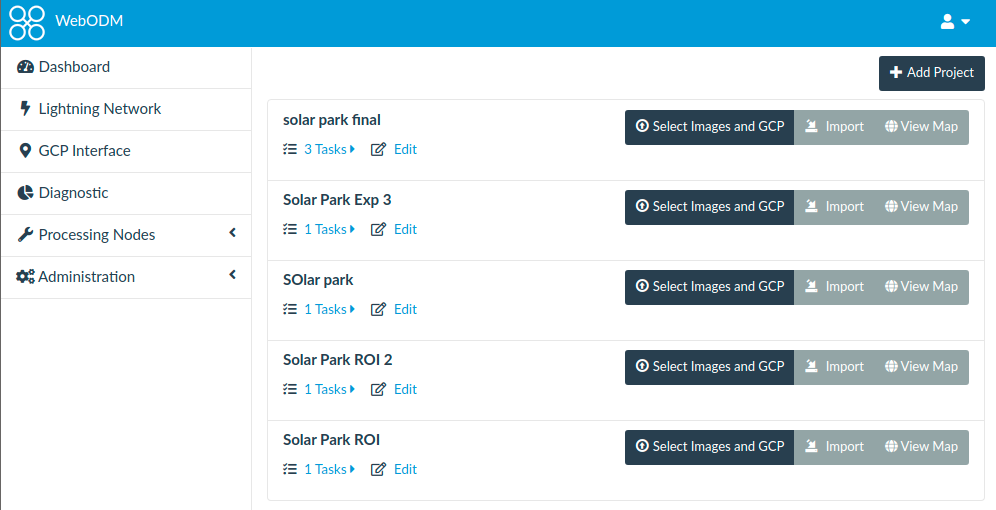
\includegraphics[width=6in]{figures/methodology/webodm}
	\label{fig:webodm}
\end{figure}

\subsection{Pegasus\_fov}
Pegasus\_fov will be a helper node to assist the operator in selecting a good grid size for the viewpoints. It will calculate the area covered by an image given the operational height of the drone and the camera calibration file. Camera calibration file has:

\begin{itemize}
	\item $w$. Image width.
	\item $h$. Image height.
	\item $K$. Camera matrix, where 
	$$K = \begin{bmatrix}
	f_x && s   && x_0 \\
	0   && f_y && y_0 \\
	0   && 0   && 1
	\end{bmatrix}$$
\end{itemize}

$f_x$ and $f_y$ are $x$ and $y$ focal length. $x_0$ and $y_0$ are principal point offset. $s$ is the axis skew.

To find the angle of view,
$$ \theta_x = 2 \times \tan^{-1}(\frac{w}{2 \times f_x}) $$

$$ \theta_y = 2 \times \tan^{-1}(\frac{h}{2 \times f_y}) $$

From $\theta_x$ and $\theta_y$, the area of coverage per viewpoint from altitute $z$ can be calculated.

$$ x = 2 \times \tan(\frac{\theta_x}{2}) \times z $$
$$ y = 2 \times \tan(\frac{\theta_y}{2}) \times z $$ 

$(x, y)$ will be the area captured by the camera at altitude $z$. The operator can use this information to choose the size of the grids in path planning.

This node will be accessible using rosrun with parameters \_camera\_file and \_height as follows:

\begin{verbatim}
$ rosrun pegasus_uav_ros pegasus_fov.py 
    _camera_file:=$(pwd)/src/pegasus_uav_ros/calibration/mobius.yaml 
    _height:=20
\end{verbatim}

\section{Chapter Summary}
All chapters except Chapter 1 must include an introductory paragraph/s and a chapter summary.

\FloatBarrier
    % set 0.5 inch indentation
\setlength{\parindent}{0.5in} 
% set paragraph space = 0 space
\setlength{\parskip}{0mm}
% set line space 1.5
\setlength{\baselineskip}{1.6em}

\chapter{EXPERIMENTAL RESULTS}
\label{ch:results}
\textit{In this chapter, I run four experiments comprising three simulations with one, two and three drones and a real world experiment with one drone.  }

\section{Real World Experiment}
To test the automated system, an experiment is run in the Energy Park behind CSIM building. The site is chosen as it has structures which will help SURF descriptors recognize features. 
\subsubsection{Mesh Network}

The mesh network consists of two wireless mesh routers running OpenWrt. Both of the routers are dual channel 2.5/5 GHz's routers with two radios. The GCS wireless router is a Netgear router (Figure~\ref{fig:gcs-router}). The GCS laptop is connected to the router via 2.5GHz WiFi network with SSID UAV01\_01. The TP-Link mobile wireless router (Figure~\ref{fig:mobile-router}) mounted on the drone is connected to the companion Raspberry Pi via Ethernet. The SSID of the mesh network is UAV01\_MESH5G and is running on 5 GHz channel. Figure~\ref{fig:mesh-network-real-world} shows the network infrastructure used.

The GCS laptop and companion are not mesh clients but are connected to different networks. Route between the GCS laptop and companion Raspberry Pi is achieved by using OSLR Host and network association (HNA) message to allow connection to these networks. Since GCS laptop is connected to different subnet than the Raspberry Pi, a route \texttt{\$ sudo route add -net 192.168.41.0/24 gw 192.168.40.1 wlp0s20f3} has to be added manually in the GCS laptop to divert the packet for the Raspberry Pi's subnet via the wireless LAN interface of the GCS to the the mesh network.

The IP assignment for different nodes in the network is given in Table~\ref{tab:network-assignment}.


\begin{table}[t]
	\caption[IP assignment for real world experiment]{\small IP assignment for real world experiment}
	\begin{center}
		\begin{tabular}{c|c|c|c}
			\hline Node & IP Address & Subnet & OSLR Interface IP\\ \hline \hline
			GCS Wireless Router & 192.168.40.1 &  192.168.40.1/24 & 192.168.30.1 \\ \hline
			Mobile Wireless Router & 192.168.41.1 & 192.168.41.1/24 & 192.168.30.2   \\ \hline 
			GCS Laptop & 192.168.40.216 & 192.168.40.1/24 & -  \\ \hline 
			Companion Raspberry Pi & 192.168.41.200 & 192.168.41.1/24 & - \\ \hline
		\end{tabular}
	\end{center}
	\label{tab:network-assignment}
\end{table} 


\begin{figure}
	\centering
	\caption[Network infrastructure for real world experiment]{\small Network infrastructure for real world experiment.} 
	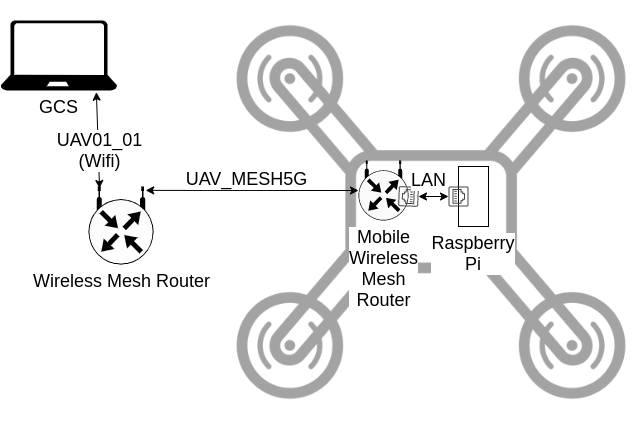
\includegraphics[width=5in]{figures/experiment/real-world-network}
	\label{fig:mesh-network-real-world}
\end{figure}

\begin{figure}
	\centering
	\caption[Wireless routers used in experiment.]{\small 
		(a) Netgear wireless router for the GCS. (b) TP-Link mobile wireless router mounted on the drone. }
	\subfloat[]{%
		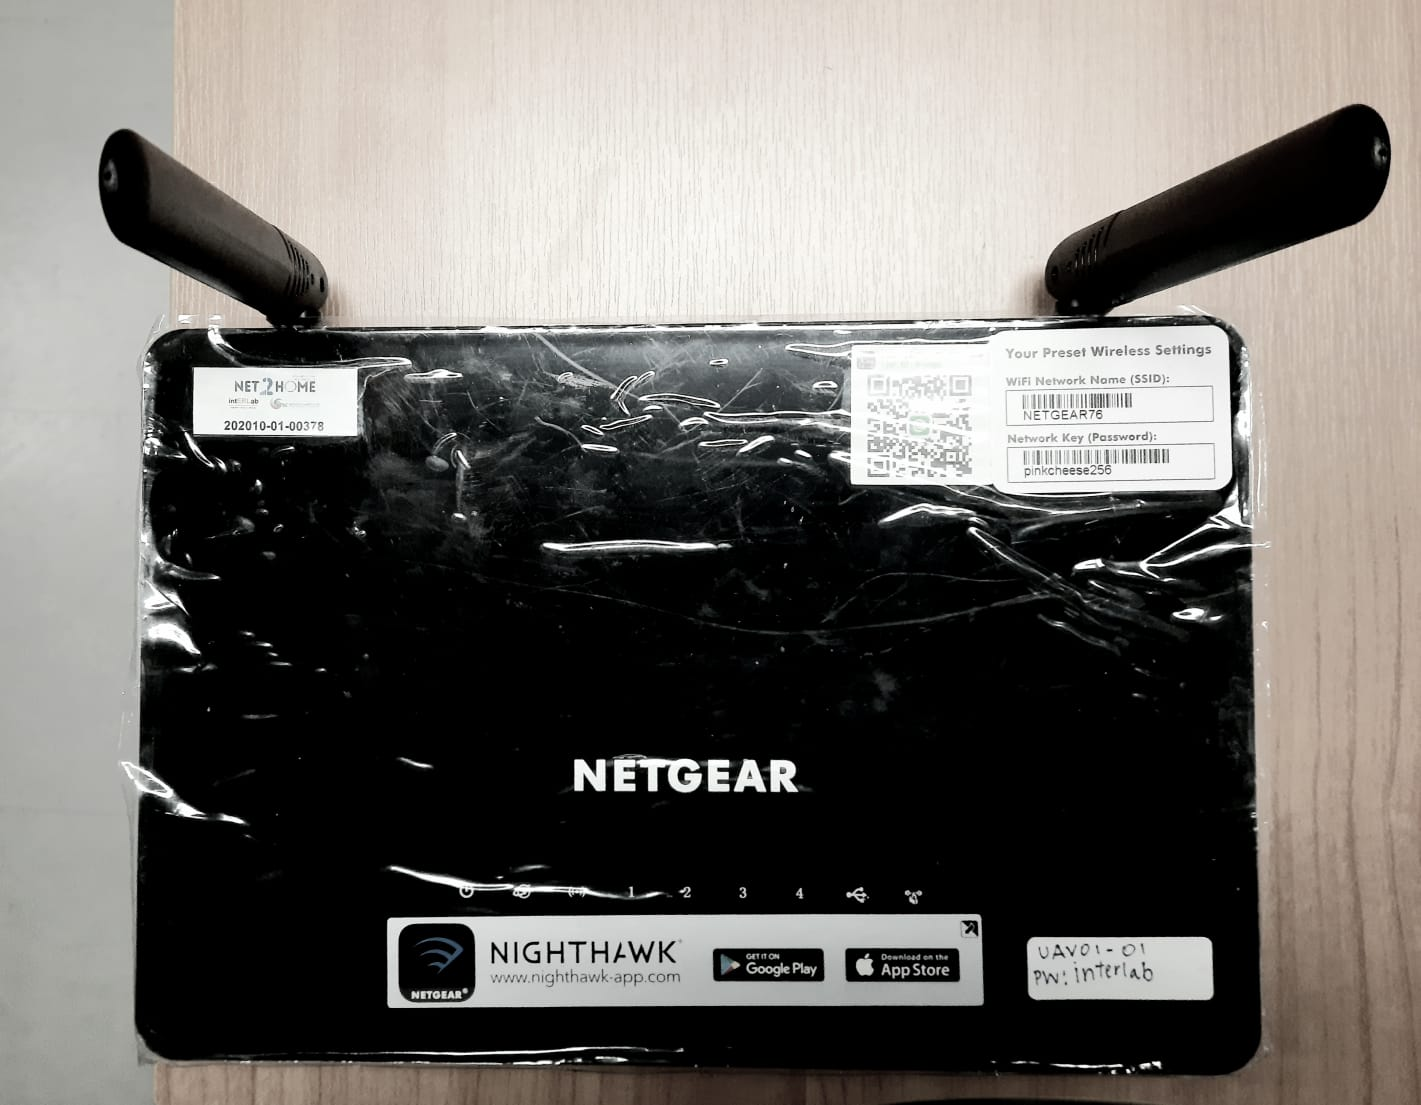
\includegraphics[width=3in]{figures/experiment/router2-mesh}
		\label{fig:gcs-router}
	}
	\subfloat[]{%
		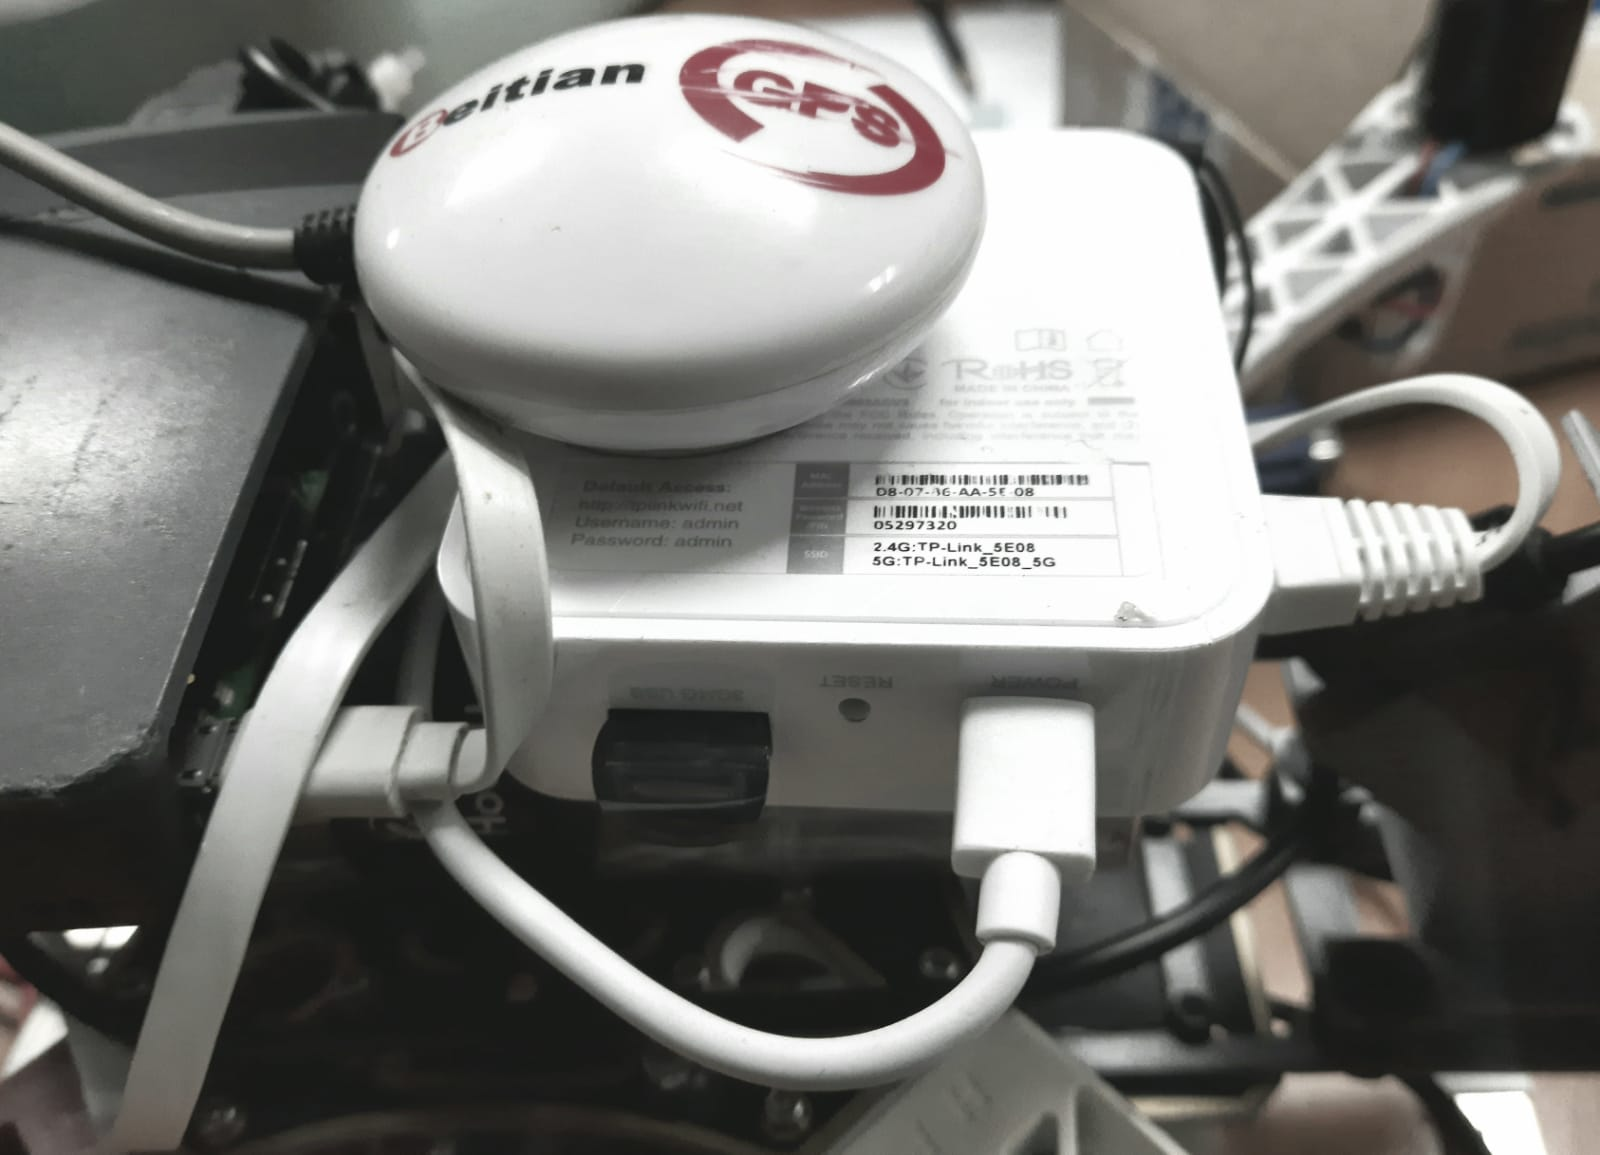
\includegraphics[width=3in]{figures/experiment/router1-mesh}%
		\label{fig:mobile-router}
	}
	
	\label{fig:real-routers}
\end{figure}

\subsection{Automated Planning}

For planning the path, the operational altitude is set at 20 meters, the grid size is set at 10 meters and the mesh range is set at 40 meters. The results of planning is given in Table~\ref{tab:real-world-planning}. The viewpoints and the path generated is shown is Figure~\ref{fig:real-path}.
\begin{table}[t]
	\caption[Result of \texttt{pegasus\_planner} in real world experiment.]{\small Result of\texttt{pegasus\_planner} in real world experiment.}
	\begin{center}
		\begin{tabular}{c|c|c|c}
			\hline Type & Number of Drones & Viewpoints Generated & Path Size \\ \hline \hline
			Real Experiment & 1 & 16 & 18 \\ \hline
		\end{tabular}
	\end{center}
	\label{tab:real-world-planning}
\end{table} 


\begin{figure}
	\centering
	\caption[Path generated for real world experiment.]{\small Path generated for real world experiment.} 
	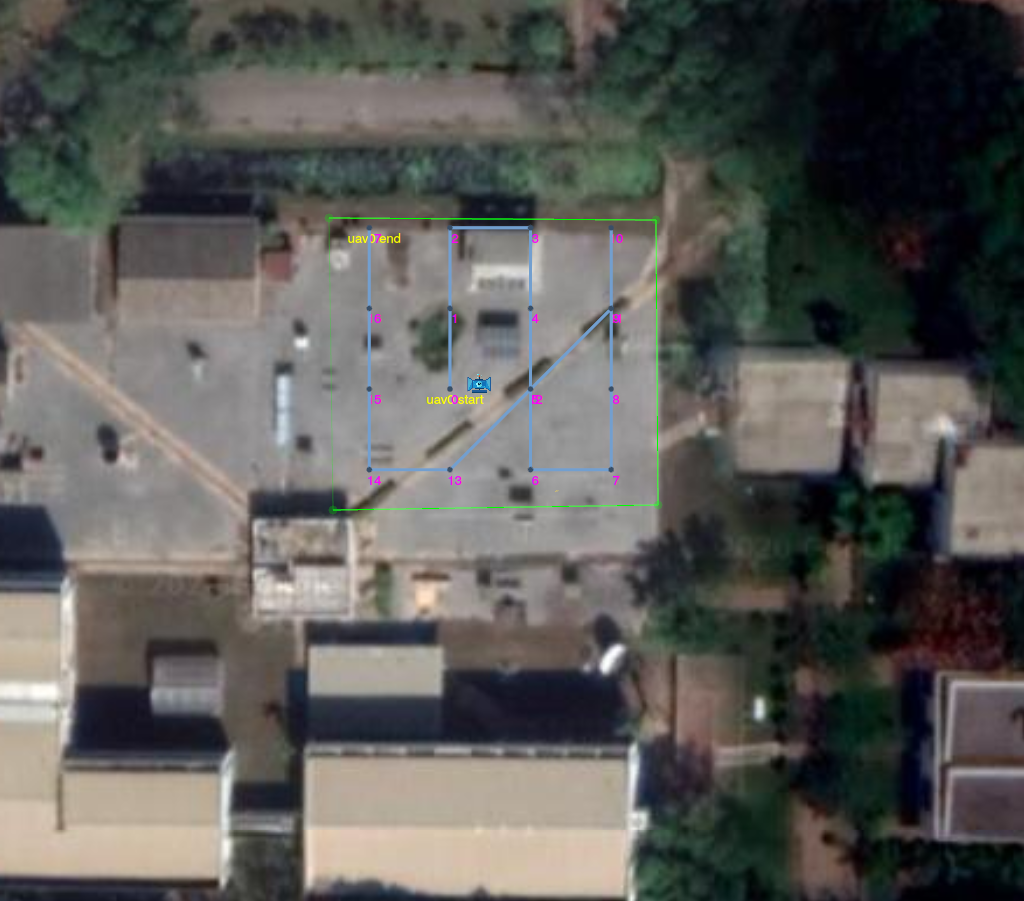
\includegraphics[width=5in]{figures/experiment/real_mapviz_plan}
	\label{fig:real-path}
\end{figure}

\subsection{Motion Control}
The pegasus\_controller was able to successfully communicate with the pegasus\_commander in the drone and control the motion of the drone in off-board mode throughout the experiment. The movement type was set to strafe to reduce the time taken for the mission as the drone would not need to align itself at yaw 0\degree after reaching each viewpoint. The pegasus\_controller was successfully able to calculate the transform between the local map of the drone and the global map after the calibration routine. To ensure the safety of the drone, the system was started with the drone in HOLD mode at 20 meters altitude. There was a slight drift in the position of the drone when it was being set to off-board mode through the companion computer. The actual path of the drone during the mission as reported by GPS data received through the heart beat reply is shown in Figure~\ref{fig:real-gps}. The figure does not show drone returning to its home position after the end of the mission because heart beat message is stopped after the drone has reached and collected image in the last pose of its path. Figure~\ref{fig:q-real-gps} shows the complete mission path in QGroundControl.


\begin{figure}
	\centering
	\caption[GPS position reported through pegasus system.]{\small GPS position reported through pegasus system.} 
	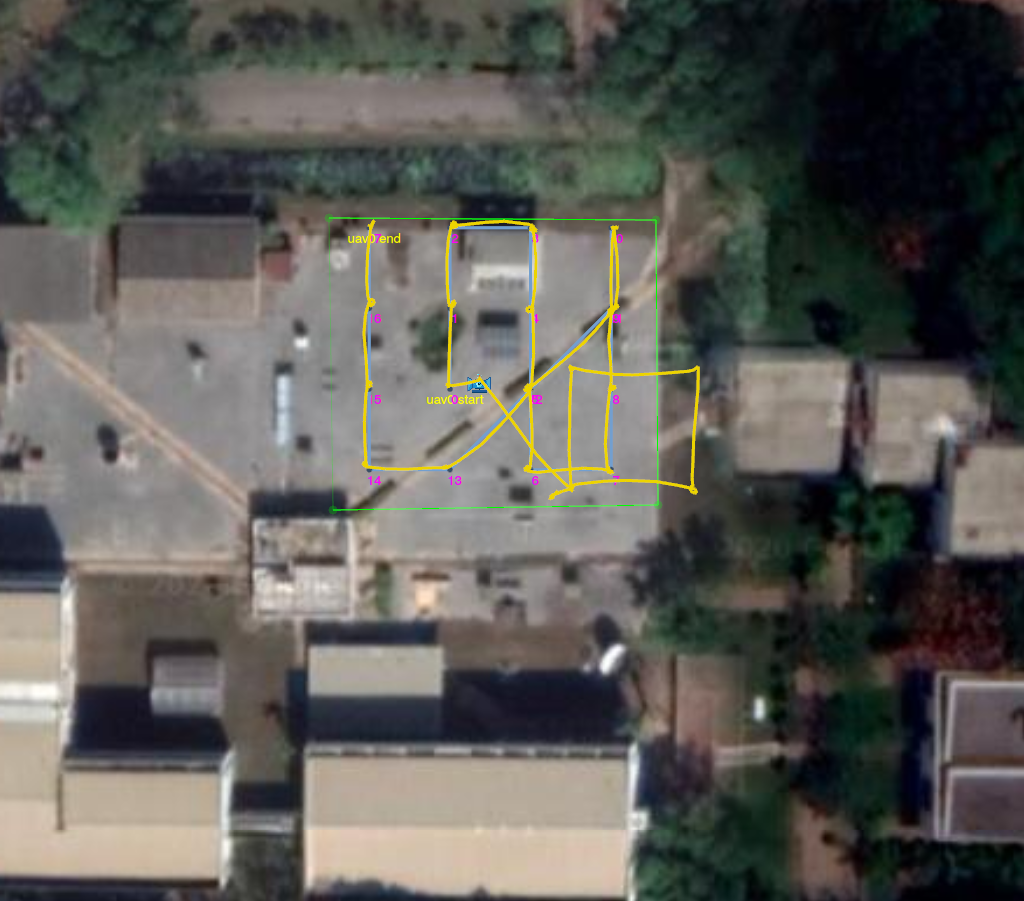
\includegraphics[width=5in]{figures/experiment/real_mapviz_path}
	\label{fig:real-gps}
\end{figure}

\begin{figure}
	\centering
	\caption[GPS position reported through telemetry wifi.]{\small GPS position reported through telemetry WiFi in QGroundControl.} 
	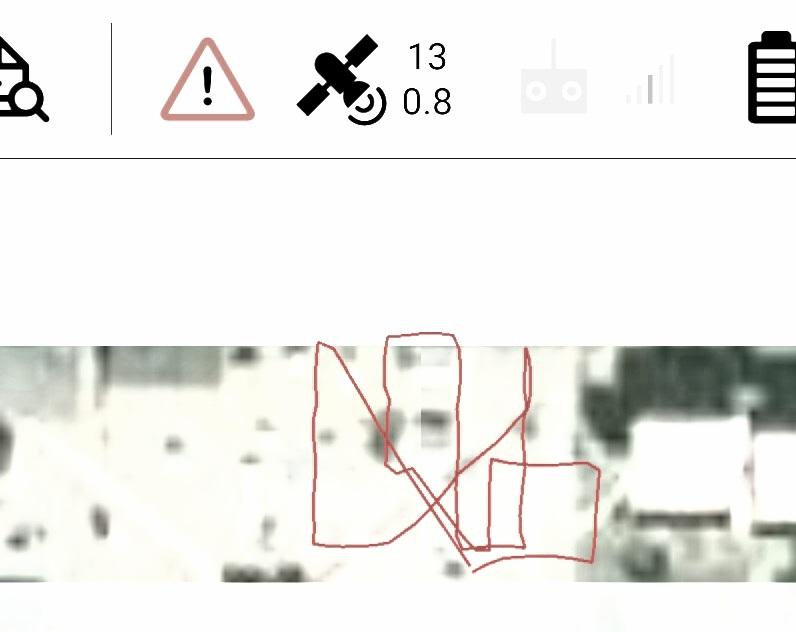
\includegraphics[width=5in]{figures/experiment/q-ground-control}
	\label{fig:q-real-gps}
\end{figure}


\subsection{Images Captured}

The pegasus\_image\_subscriber and pegasus\_image\_publisher successfully acquired 16 images from 16 viewpoints in the mission in real-time as shown in Figure~\ref{fig:real-images}. Using an application called photini, the location of the images can be seen in Figure~\ref{fig:exif-real-images}. 
\begin{figure}
	\centering
	\caption[Images captured by pegasus in real-time.]{\small Images captured by pegasus in real-time.} 
	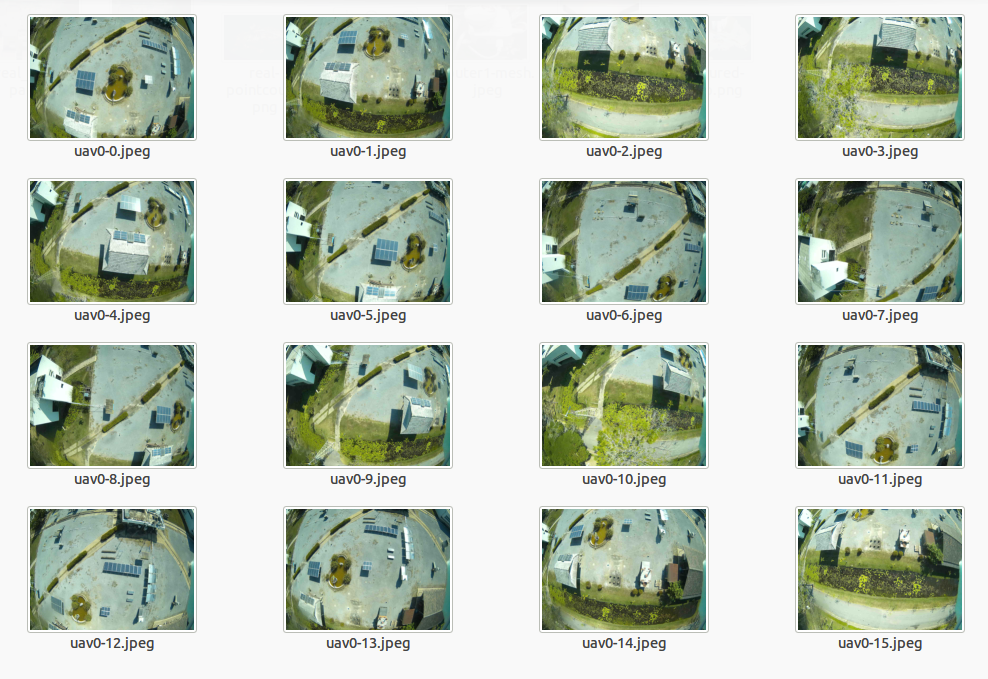
\includegraphics[width=6in]{figures/experiment/real-images}
	\label{fig:real-images}
\end{figure}

\begin{figure}
	\centering
	\caption[Location of images captured.]{\small Location of images captured.} 
	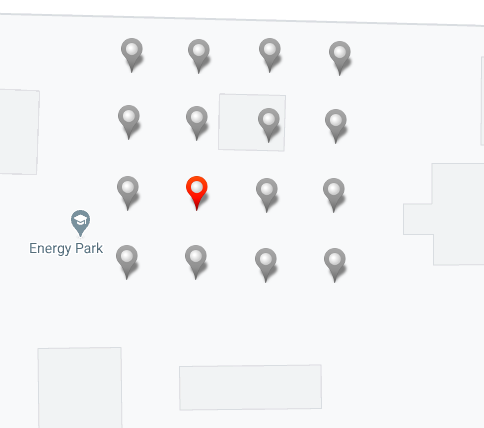
\includegraphics[width=5in]{figures/experiment/real-images-exif-tag}
	\label{fig:exif-real-images}
\end{figure}

\subsection{Result}
The images captured is rectified using pegasus\_image\_rectify using the camera calibration file. Then the rectified images are processed using WebODM.
\begin{itemize}
	\item Figure~\ref{fig:orthophoto-real} shows the orthophoto of the region of interest.
	\item Figure~\ref{fig:real-pointcloud} shows the point cloud of the region of interest.
	\item Figure~\ref{fig:real-textured-map} shows the textured model of the region of interest.
	\item Figure~\ref{fig:real-camera-position} shows the camera position as determined by ODM of the region of interest.
\end{itemize}

\begin{figure}
	\centering
	\caption[Orthophoto of Energy Park.]{\small Orthophoto of Energy Park.} 
	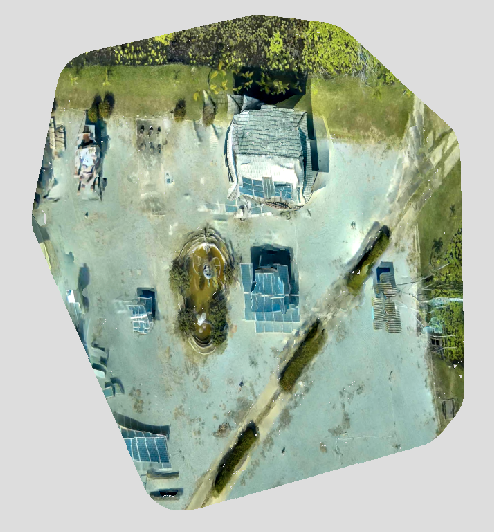
\includegraphics[width=5in]{figures/experiment/orthophoto-real}
	\label{fig:orthophoto-real}
\end{figure}

\begin{figure}
	\centering
	\caption[Point cloud of Energy Park.]{\small Point cloud of Energy Park.} 
	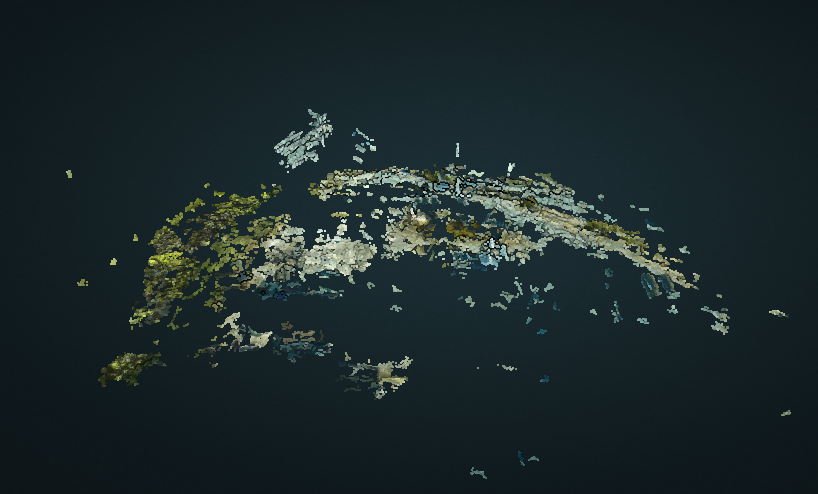
\includegraphics[width=5in]{figures/experiment/real-pointcloud}
	\label{fig:real-pointcloud}
\end{figure}

\begin{figure}
	\centering
	\caption[Textured mesh of Energy Park.]{\small Textured model of Energy Park.} 
	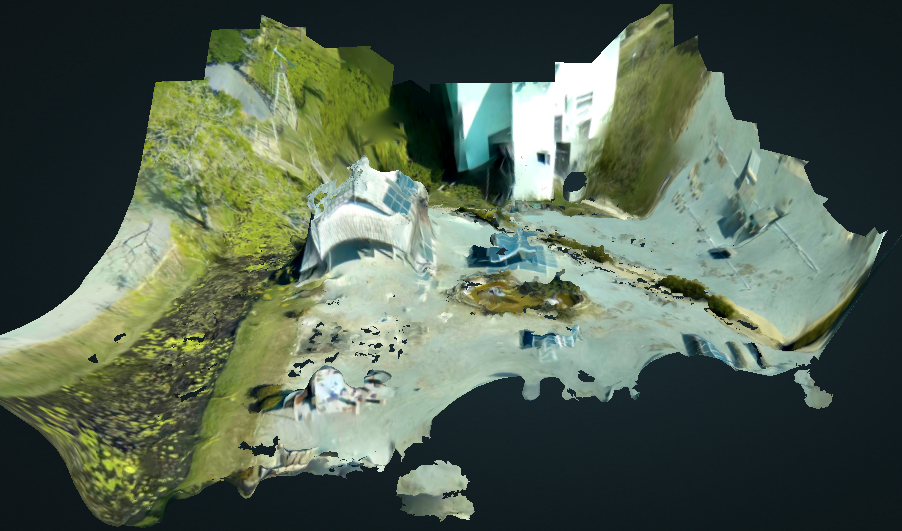
\includegraphics[width=5in]{figures/experiment/real-textured-map}
	\label{fig:real-textured-map}
\end{figure}

\begin{figure}
	\centering
	\caption[Camera Position calculated by ODM.]{\small Camera Position calculated by ODM.} 
	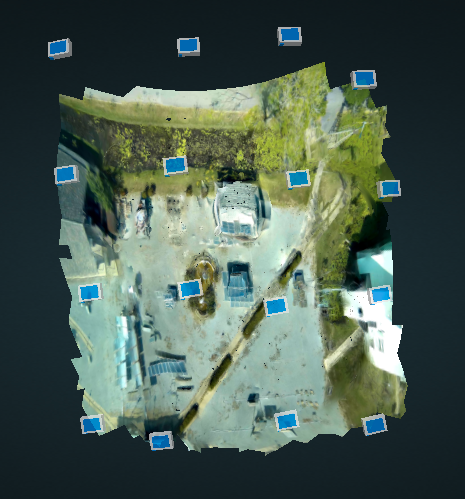
\includegraphics[width=5in]{figures/experiment/camera-position}
	\label{fig:real-camera-position}
\end{figure}

\section{Simulation}

Simulation will be run on the Gazebo world shown in Figure~\ref{fig:sim-world}. Simulation experiment will use 3 drones. 

\begin{figure}
	\centering
	\caption[Gazebo simulation world.]{\small Gazebo simulation world 
		(a) Top View. (b) Side View. }
	\subfloat[]{%
		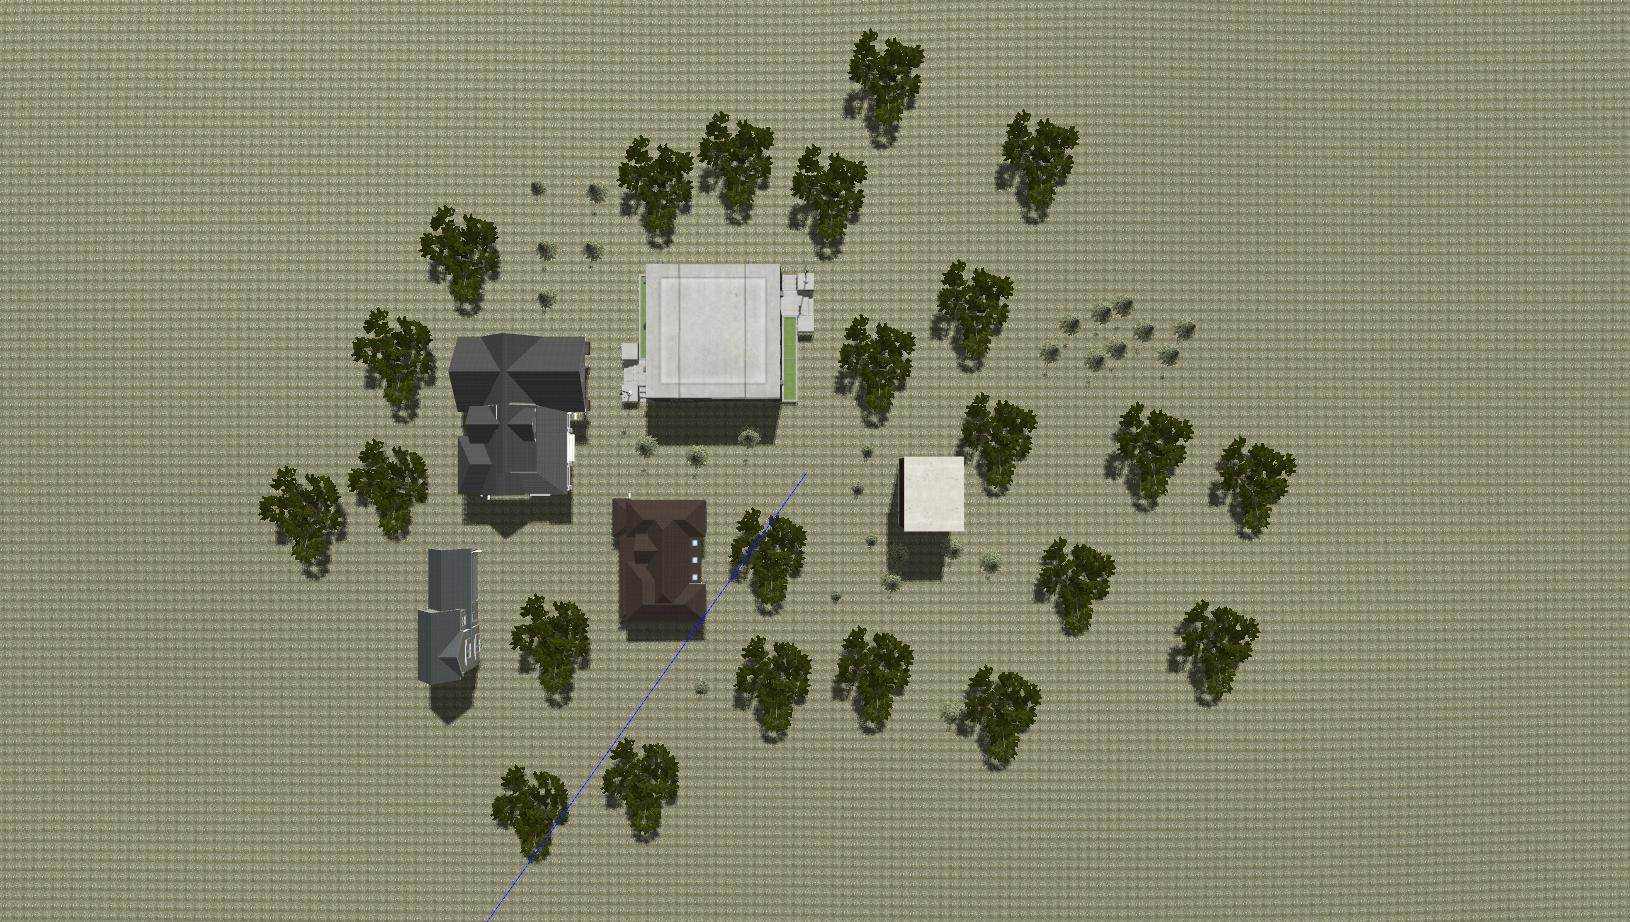
\includegraphics[width=5in]{figures/experiment/sim-world1}
	}
	
	\subfloat[]{%
		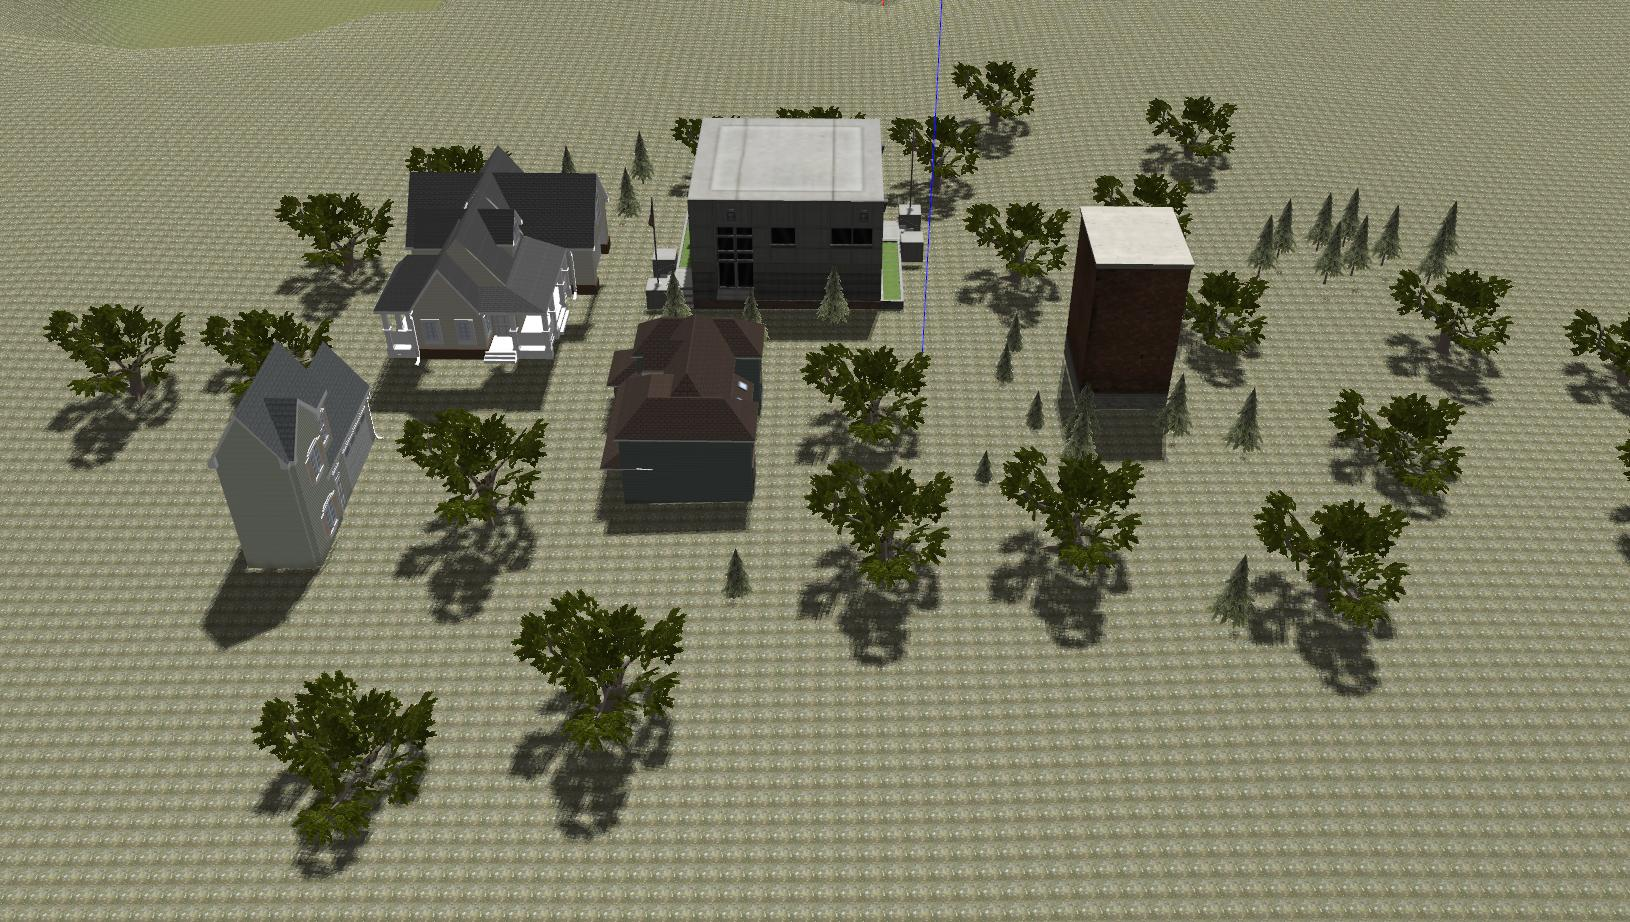
\includegraphics[width=5in]{figures/experiment/sim-world2}%
	}
	\label{fig:sim-world}
\end{figure}

\subsection{Simulated Network Configuration}

All the network packets will be routed though ns3. ns3 is configured with 3 drones each having a pegasus\_commander and pegasus\_controller. Therefore the GCS mush have a total of six udp sockets to control the system of three drones. The pegasus-net-sim ns3 simulator is configured as follows:

\begin{verbatim}
std::map<std::string, std::vector<PegasusPortConfig>> 
PegasusConfig::m_config {
{
"iris_0", {
{5444, 4444, 3444},
{7300, 7400, 7200},
}
},
{
"iris_1", {
{5445, 4445, 3445},
{7301, 7401, 7201},
}
},
{
"iris_2", {
{5446, 4446, 3446},
{7302, 7402, 7202},
}
},
{
CONTROL_STATION_STR , {
{3444, 6444, 5444},
{7200, 8200, 7300},
{3445, 6445, 5445},
{7201, 8201, 7301},
{3446, 6446, 5446},
{7202, 8202, 7302},
}
},
};
\end{verbatim}

\subsection{Automated Planning}
The area of interest is larger than the real world experiment with one drone and has more viewpoints. The operational height for the simulation is set at 30 meters. The grid size is set at 10 meters. The mesh range is set at 40 meters. The planning is completed at 3.74 seconds. The result of the planning is given in Table~\ref{tab:simulated-planning}. The path planned by the planner is shown in Figure~\ref{fig:simulated-plan}.

\begin{table}[t]
	\caption[Result of \texttt{pegasus\_planner} in simulated experiment with three drones.]{\small Result of \texttt{pegasus\_planner} in simulated experiment with three drones.}
	\begin{center}
		\begin{tabular}{c|c|c|c}
			\hline Type & Number of Drones & Viewpoints Generated & Path Size \\ \hline \hline
			Simulation & 3 & 25 & 11, 11, 10 \\ \hline
		\end{tabular}
	\end{center}
	\label{tab:simulated-planning}
\end{table}

\begin{figure}
	\centering
	\caption[Paths generated for three drones in simulation experiment.]{\small Paths generated for three drones in simulation experiment.} 
	\includegraphics[width=5in]{figures/experiment/simulated-plan}
	\label{fig:simulated-plan}
\end{figure}

\subsection{Motion Control}
The pegasus\_controller is able to control three drones at once though pegasus\_commander in the drones. The transformation between the local maps of the drones and the global map is successfully calculated. pegasus\_controller is able to successfully carry out the coordinated mission without the drones colliding with each other.  The path taken by the drones are shown in Figure~\ref{fig:simulated-path}.

\begin{figure}
	\centering
	\caption[The path followed by the drones as reported through the simulated GPS of the drones.]{\small The path followed by the drones as reported through the simulated GPS of the drones.} 
	\includegraphics[width=5in]{figures/experiment/simulated-path}
	\label{fig:simulated-path}
\end{figure}

\subsection{Image Acquisition}
Thirty images were acquired from the 3 drones in real time. The images are captured with gst (gstreamer) camera plugin for gazebo and do not have any distortion. The captured images are shown in Figure~\ref{fig:simulated-images}. The position of images as described by the EXIF tag is shown in Figure~\ref{fig:simulated-images-position}.
\begin{figure}
	\centering
	\caption[The images captures in real-time during simulation.]{\small The images captured in real-time during simulation.} 
	\includegraphics[width=6in]{figures/experiment/simulated-images}
	\label{fig:simulated-images}
\end{figure}
\begin{figure}
	\centering
	\caption[The GPS location of the images captured during simulation.]{\small The GPS location of the images captured during simulation.} 
	\includegraphics[width=5in]{figures/experiment/simulated-image-position}
	\label{fig:simulated-images-position}
\end{figure}

\subsection{Results}
The network traffic and the ODM outputs are analyzed for the simulation.

\subsubsection{Network Properties}
The traffic in the simulated network is captured in pcap format and wireshark is used to analyse the traffic. The distribution packet size is given in Table~\ref{tab:packet-size}. The ratio of protocol in the network is given in Table~\ref{tab:packet-protocol}. The amount of traffic generated by pegasus system for control and image messages are given in Table~\ref{tab:traffic-generation}.

\begin{table}[t]
	\caption[Distribution of packet size in the simulated network.]{\small Distribution of packet size in the simulated network.}
	\begin{center}
		\begin{tabular}{llllll}
			\hline Packet Lengths   & Count  & Average Length & Min Length & Max Length & Percent \\ \hline \hline
			All              & 217479 & 166.18         & 14         & 1046       & 100\%   \\
			0-19             & 45799  & 14             & 14         & 14         & 21.06\% \\
			20-39            & 0      & -              & -          & -          & 0.00\%  \\
			40-79            & 68814  & 74.15          & 45         & 78         & 31.64\% \\
			80-159           & 82414  & 115.43         & 80         & 122        & 37.90\% \\
			160-319          & 122    & 182.59         & 175        & 270        & 0.06\%  \\
			320-639          & 566    & 343.41         & 323        & 568        & 0.26\%  \\
			640-1279         & 19764  & 1045.66        & 669        & 1046       & 9.09\%  \\
			1280-2559        & 0      & -              & -          & -          & 0.00\%  \\
			2560-5119        & 0      & -              & -          & -          & 0.00\%  \\
			5120 and greater & 0      & -              & -          & -          & 0.00\% \\  \hline
		\end{tabular}
	\end{center}
	\label{tab:packet-size}
\end{table}

\begin{table}[t]
	\caption[Protocol distribution in the simulated network.]{\small Protocol distribution in the simulated network.}
	\begin{center}
		\begin{tabular}{lllll}
			\hline Protocol                              & Percent Packets & Packets & Percent Bytes & Bytes    \\ \hline \hline
			Malformed Packet                      & 0.15            & 335     & 0.000         & 0        \\
			Logical-Link Control                  & 47.33           & 102928  & 73.296        & 26488790 \\
			Internet Protocol Version 4           & 47.29           & 102836  & 5.691         & 2056720  \\
			User Datagram Protocol                & 47.29           & 102836  & 2.276         & 822688   \\
			Real-time Transport Control  & 0.02            & 36      & 0.065         & 23472    \\
			Optimized Link State Routing  & 27.18           & 59120   & 7.194         & 2599896  \\
			Data                                  & 20.07           & 43647   & 54.640        & 19746698 \\
			Address Resolution Protocol           & 0.04            & 92      & 0.007         & 2576     \\ \hline
		\end{tabular}
	\end{center}
	\label{tab:packet-protocol}
\end{table}

\begin{table}[t]
	\caption[ Traffic generated by pegasus system.]{\small Traffic generated by pegasus system.}
	\begin{center}
		\begin{tabular}{lllllll}
			\hline Address A & Port A & Address B & Port B & Packets & Bytes   & Type   \\ \hline \hline
			10.1.3.2  & 5444   & 10.1.3.1  & 3444   & 517     & 105753  & motion \\
			10.1.3.2  & 7300   & 10.1.3.1  & 7200   & 12122   & 6619985 & Image  \\
			10.1.3.3  & 5445   & 10.1.3.1  & 3445   & 390     & 79439   & motion \\
			10.1.3.3  & 7301   & 10.1.3.1  & 7201   & 15829   & 8519059 & Image  \\
			10.1.3.4  & 5446   & 10.1.3.1  & 3446   & 464     & 95158   & motion \\
			10.1.3.4  & 7302   & 10.1.3.1  & 7202   & 14394   & 7762232 & Image  \\ \hline
		\end{tabular}
	\end{center}
	\label{tab:traffic-generation}
\end{table}

\subsubsection{Map building}
The images do not have distortion, hence they are directly processed using WebODM.
\begin{itemize}
	\item Figure~\ref{fig:orthophoto-simulated} shows the orthophoto of the region of interest.
	\item Figure~\ref{fig:simulated-pointcloud} shows the point cloud of the region of interest.
	\item Figure~\ref{fig:textured-map-simulated} shows the textured model of the region of interest.
	\item Figure~\ref{fig:simulated-camera-position} shows the camera position as determined by ODM of the region of interest.
\end{itemize}

\begin{figure}
	\centering
	\caption[Orthophoto of simulated region of interest.]{\small Orthophoto of simulated region of interest.} 
	\includegraphics[width=5in]{figures/experiment/orthophoto-simulated}
	\label{fig:orthophoto-simulated}
\end{figure}

\begin{figure}
	\centering
	\caption[Point cloud of simulated region of interest.]{\small Point cloud of simulated region of interest.} 
	\includegraphics[width=5in]{figures/experiment/simulated-pointcould}
	\label{fig:simulated-pointcloud}
\end{figure}

\begin{figure}
	\centering
	\caption[Textured mesh of simulated region of interest.]{\small Textured mesh of simulated region of interest.} 
	\includegraphics[width=5in]{figures/experiment/textured-simulated}
	\label{fig:textured-map-simulated}
\end{figure}

\begin{figure}
	\centering
	\caption[Position of simulated camera calculated by ODM.]{\small Position of simulated camera calculated by ODM.} 
	\includegraphics[width=5in]{figures/experiment/simulated-camera}
	\label{fig:simulated-camera-position}
\end{figure}

\section{Chapter Summary}
All chapters except Chapter 1 must include an introductory paragraph/s and a chapter summary.


\FloatBarrier
    % set 0.5 inch indentation
%\setlength{\parindent}{0.5in}
\setlength{\parindent}{0pt} 
% set paragraph space = 0 space
\setlength{\parskip}{0mm}
% set line space 1.5
\setlength{\baselineskip}{1.6em}

\chapter{CONCLUSION}
\label{ch:conclusion}

The thesis study is concluded in this chapter and recommendations for future work is provided. The system is able to run in simulation with multiple drones and it has been evaluated in the real world with one drone. 

\section{Conclusion}
I propose a system to autonomously survey a region of interest using multiple drones connected to a wireless mesh network using a ground control station to coordinate their movements in my thesis study. Furthermore, the system is capable of acquiring geo-tagged images from the drones in real time, which can be used after the mission is complete to build a 3D model and orthophoto image of the region of interest. One of the use cases of the Pegasus system is to survey an area after a disaster using multiple drones autonomously. Multiple drones can survey a region of interest in a shorter amount of time than a single drone. Thus, cost effective drones can be used despite the constraints of short battery life.

The system provides the operator with an interface to select the area of interest to survey. Viewpoints are generated in the area of interest. An iterative A* search algorithm is used find an efficient path for the drones to cover the viewpoints without losing mesh network coverage or colliding with each other. Since the problem of finding the optimal paths for the drones to cover all the viewpoints is NP-hard, the A* algorithm is tweaked to provide reasonable solutions in a reasonable amount of time. This forms the planning facet of the system.

The drones are controlled in real time by a centralized ground control station connected to the mesh network. Each of the drones and the GCS operate in different local frames of reference. The system finds the transformation between all local frames of reference and the global frame of reference through a predefined calibration routine that is run before the drones start following their planned paths. Then each drone operates within its local map while following planned paths calculated in the global map. The GCS instructs each drone to go to a desired location with a desired orientation. If the drone loses communication with the GCS, the drone returns to its home position autonomously. This forms the motion control aspect of the system.

The GCS acquires geo-tagged images from the drones in real time using the mesh network. This forms the image acquisition part of the system. 
Finally, the images acquired during the mission from the drone are rectified and processed with WebODM. This is the map-building part of the system.

The system was tested through simulation with popular simulation tools. PX4 SITL, Gazebo and ns-3 were integrated and used together to simulate the working of the system with three drones. Simulation showed that the system will work with multiple drones. It also showed that the traffic generated by the system between the drones and the GCS is only a few megabytes, mostly for image acquisition. 

The system was also tested in the real world using one real drone. The system was able to control the motion of the drone in real time, plan a path for the area of interest, and acquire images from the planned viewpoints during flight. The acquired images were used to build a 3D model, a textured mesh, and an orthophoto of the area the system surveyed autonomously. 

The source code for the developed system is available at the Github repository \\  \url{https://github.com/rmukhia/pegasus}.
\section{Recommendations}

The system is unsafe, that is, it does not have obstacle avoidance and dynamic path adjustment. It also does not have fail-safe mechanisms for fatal conditions such as low battery in the drone. If the battery becomes low enough, the drone will simply fall to the ground from whatever altitude it is at. The system can be made more safe by integrating sensors in the drones to avoid surrounding obstacles. The system can also be extended to include real-time monitoring of the battery level of the drones to execute fail-safe behavior if the battery level falls below a particular threshold.

Currently, the system is complicated to set up. There are many ROS nodes and launch files required to execute the system. Further work can be done to make the system easier to access.

Using a higher quality camera with less radial distortion and higher resolution on the drone will provide better results, but the companion computer may need to be upgraded to handle a higher resolution video feed.


\section{Chapter Summary}
This chapter provides the conclusion and result of the study. Recommendations to further improve the system are mentioned in the chapter.

\FloatBarrier
    
    % ====== Reference part ======
    % https://ctan.math.illinois.edu/macros/latex/contrib/apacite/apacite.pdf
    \addcontentsline{toc}{part}{REFERENCES}
    % change page title
    \renewcommand\bibname{REFERENCES}
    \bibliographystyle{apacite}
    \bibliography{references}
    % ====== ======
    \addtocontents{toc}{\bf{APPENDICES}}
    % add to Table of content
% \addcontentsline{toc}{section}{\bf{APPENDIX A: SURVEY QUESTIONNAIRE}}

% set 0 indentation
\setlength{\parindent}{0pt}
% set paragraph space = 1 space
\setlength{\parskip}{1em}
% set line space = 1.5
\setlength{\baselineskip}{1.5em}



    % add to Table of content
\addcontentsline{toc}{section}{\bf{APPENDIX B: TITLE}}

% set 0 indentation
\setlength{\parindent}{0pt}
% set paragraph space = 1 space
\setlength{\parskip}{1em}
% set line space = 1.5
\setlength{\baselineskip}{1.5em}

\renewcommand{\thefigure}{B\arabic{figure}}
\renewcommand{\thetable}{B\arabic{table}}

    
\end{document}


